\chapter{Deep Learning Models}
In this chapter, we will present three models based on
different architectures: the first, our baseline, is based on a
Multi-Layer Perceptron, which will be the most basic one.
The second model is based on a Recurrent Neural Network, and finally,
the last one utilizes the newer and more powerful Transformer layers.
We will describe in detail their architecture, the various training phases,
and any associated issues along with their strengths and weaknesses
for each model.

It's important to note that these models were implemented using only
the PyTorch library.
Each run was preceded by setting a seed (the same for all runs of each model)
to allow for comparisons and ensure the repeatability of the
various operations. For training phase, the dataset created in the
previous Chapter (\ref{chap:datapreprocessing}) was used and divided
into training, validation, and testing sets as described in Section~\ref{sec:datasetsplitting}.
All of these phases were executed on a machine with 64 GB (2x32GB) DDR5 5600MT/s of RAM,
an AMD Ryzen 9 7950X3D processor, and an Nvidia 4090 GPU.

%In questo capitolo andremo a proporre 3 modelli differenti basati 
%su diverse architetture: il primo, la nostra baseline, basato
%su Multi Layer Perceptrion che risulterà quello più basilare, il secondo
%basato su Recurrent Neural Network ed infine l'ultimo che sfrutta
%i più nuovi e performanti Transofrmer layers. Andremo a descrivere
%nel dettaglio la loro architettura, le varie fasi di training e gli
%eventuali problemi con i relativi punti di forza e svantaggi per ogni 
%modello.
%
%\'{E} importante far notare che questi modello sono stati scritti usano
%solo la libreria \verb|pytorch|, ogni run è stata precedura dall'impostazione
%di un seed (uguale per tutte le run di ogni modello) per rendere possibile
%effettuare vari confronti e rendere ripetibili le varie operazioni.
%Per l'allenamento è stato utilizzato il dataset creato nel capitolo precedente (\ref{chap:datapreprocessing}) e suddiviso in training, validation e testing set come descritto nella Sezione 2.2.
%Tutte queste fasi sono state fatte eseguire sun una macchina con 64 GB di RAM,
%un AMD Ryzen 9 7950X3D e una GPU Nvidia 3090.
%
\section{MLP}\label{sec:mlpbaseline}
In this section, we will introduce the first model, which we will refer to as the
baseline model, based on a Multi-Layer Perceptron.
We will analyze its architecture, the training phase, and its final performance.

%In questa sezione andremo ad introdurre il primo modello a cui faremo
%riferiento come baseline model, basato su MultiLayer Perceptron.
%Analizzeremo la sua architettura, la 
%fase di training e le sue performance finali.

\subsection{Architecture}
This neural network is designed to predict the instantaneous energy output over
a period of exactly 2 days.
To do this, it requires input data that includes the performance of the system
(features selected during the Preprocessing phase, see Chapter \ref{chap:datapreprocessing}) for exactly one day
before and one day after the period in question.
This enables it to understand how the system is performing and,
consequently, provide the energy output trend.
The model consists of 6 main layers:

%Questa rete neurale è progettata per prevedere l'andamento dell'energia istantanea prodotta durante un periodo di un buco di esattamente 2 giorni.
%Per farlo ha bisogno di avere come input l'andamento dell'impianto (features selezionate nella fase di preprocessing) di esattamente un giorno prima del
%buco e di un giorno dopo. In questo modo può riuscire a comprendere come l'impianto sta performando e quindi restituire l'andamento dell'energia.
%Il modello è formato da 6 livelli principali:

\begin{figure}[H]
	\begin{minipage}{0.6\textwidth}
		\begin{itemize}
			\item \textbf{Input layer}: This is the first layer of the network.
			      It takes two input tensors: \textit{before} and \textit{after}.
			      These tensors represent the day before and the day after the specific period we want to
			      predict. They have the shape \verb|[BATCH_SIZE, 96, 33]|, where 96 is the number
			      of timestamps in our dataset that make up one day, and 33 represents the
			      features obtained from the Data Preprocessing phase.
			      These tensors are then flattened and concatenated to be passed to the subsequent layer.
			      The output of this layer goes through a Batch Normalization layer, and the
			      Rectified Linear Unit (ReLU) activation function is used.

			      % è il primo livello della rete, prende in input 2 tensori: \textit{before} e \textit{after}. Questi stanno ad indicare rispettivamente il giorno prima e quello dopo del buco che vogliamo chiudere. Avranno la forma \verb|[BATCH_SIZE, 96, 33]|, dove \verb|96| è il numero di timestamp del nostro dataset che formano un giorno e \verb|33| sono le feature ottenute dalla fase di preprocessing dei dati. A questi verrà poi applicata un'operazione di Flatten ed infine concatenati per poter essere poi passati al layer successio.
			      %L'output di questo layer passa per un livello di Batch Normalization e viene utilizzata la ReLu come funzione di attivazione. 

			\item \textbf{Hidden layers}: In total, there are 4 layers, each of which takes the
			      output of the previous layer as input and reduces the number of neurons by half.
			      Batch Normalization is applied to the result, and the Rectified Linear Unit (ReLU)
			      is used as the activation function.

			      %in totale 4, ognuno prende in input il risultato del layer precedente e va a dimezzare il numero dei neuroni. Al risultato viene applicata un'operazione di Batch Normalization e utilizzata la ReLu come funzione di attivazione.

			\item \textbf{Output layer}: The final layer of our network, it takes the result from the
			      previous layer and outputs the value of the Instantaneous Energy Produced
			      during the specific period.
			      It produces a tensor with a shape of \verb|[BATCH_SIZE, 192, 1]|.
			      The SoftPlus function is used as the final activation function.

			      %ultimo layer della nostra rete, dal risultato del layer precedente riporta come output il valore dell'Energia Istantanea Prodotta durante il buco, un tensore di forma \verb|[BATCH_SIZE, 192, 1]|. Viene utilizzata la SoftPlus come funzione di attivazione finale.
		\end{itemize}
	\end{minipage}%
	\hspace{0.5cm}
	\begin{minipage}{0.4\textwidth}
		\centering
		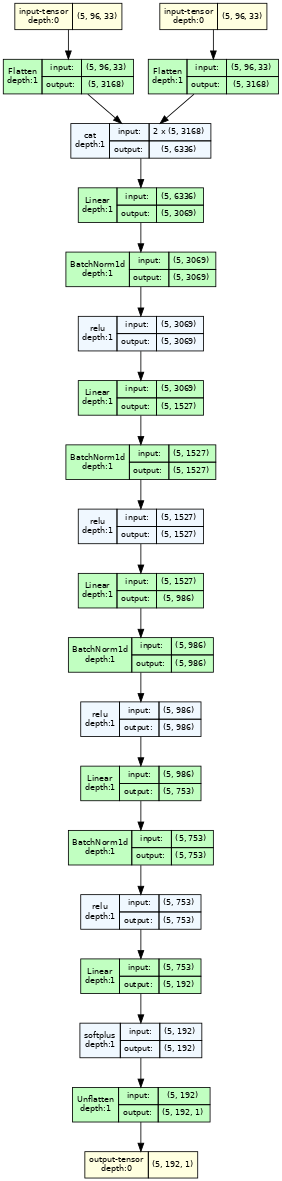
\includegraphics[width=0.5\textwidth]{chapters/3_models/imgs/ufcnmodel.png}
		\caption{Beseline Model architecture visualization.}\label{fig:baselinemodelarch}
	\end{minipage}
\end{figure}

\begin{minipage}[t]{0.5\textwidth}
	\begin{figure}[H]
		\centering
		\begin{tikzpicture}
			\draw[->] (-3,0) -- (3,0) node[right] {$x$};
			\draw[->] (0,-1) -- (0,4) node[above] {$y$};
			\draw[dotted] (-3,-1) grid (3,4);
			\draw[color=blue, domain=-3:0] plot[id=logistic] function{0};
			\draw[color=blue, domain=0:3] plot[id=logistic] function{x};
		\end{tikzpicture}
		\caption{Rectified Linear Unit function. $ReLu(x) = \max(0, x)$}
		\label{fig:relu}
	\end{figure}
\end{minipage}%
\hspace{.5cm}
\begin{minipage}[t]{0.5\textwidth}
	\begin{figure}[H]
		\centering
		\begin{tikzpicture}
			\draw[->] (-3,0) -- (3,0) node[right] {$x$};
			\draw[->] (0,-1) -- (0,4) node[above] {$y$};
			\draw[dotted] (-3,-1) grid (3,4);
			\draw[color=blue, domain=-3:3] plot[id=logistic] function{log(1+exp(x))};
		\end{tikzpicture}
		\caption{SoftPlus function. $SoftPlus(x) = \frac{1}{\beta} \log(1+e^{\beta x})$}
		\label{fig:softplus}
	\end{figure}
\end{minipage}

\subsection{Training}
The model was trained by artificially creating gaps of two days in length within the
training dataset.
These gaps were passed to the network in the format described earlier,
and the output result was compared to the actual instantaneous energy produced during the gap.
An \textit{Early Stopping} procedure was implemented to prevent training from continuing if
the model was not improving its performance.
A procedure, called \textit{Save Best}, has also been integrated,
which saves the model to a file whenever the Validation Loss improves.
The validation dataset was applied in this phase to assess the learning progress at the end
of each epoch.
A normalization procedure of the area was applied to the model's output in relation to
that of the gap to ensure that the output starts exactly from the last value of the
instantaneous energy produced \textit{before} and ends exactly with the first value
of the energy produced \textit{after}. Adam was used as the optimizer,
and L1Loss (Equation~\ref{eq:l1loss}) served as the loss function.
We chose to set the batch size parameter to 10, the learning rate $\lambda$ to 0.01,
a maximum of 100 epochs, and a patience value of 20 for Early Stopping.

%Il modello è stato allenato creando, in modo artificiale, buchi di lunghezza
%pari a due giorni all'interno del dataset di training, passati alla rete nel formato
%descritto precedentemente e confrontato il risultato in output con l'effettiva energia istantanea
%prodotta del buco. \'{E} stata implementata una procedura di \textit{Early Stopping} per evitare
%di continuare l'allenamento anche se il modello non sta migliorando le sue performance. 
%\'{E} stata anche integrata una procedura, chiamata \textit{Save Best},
%che salva il modello su file ogni qualvolta la validation loss migliori.
%Il dataset di validation è stato applicato in questa fase per verificare lo stato di
%apprendimento alla fine di ogni epoca. All'output del modello è stata applicata una 
%procedura di normalizzazione dell'area rispetto a quella del buco per far si che la predizione
%parta esattamente dall'ultimo valore dell' energia istantanea prodotta di \textit{before} e
%termini esattamente con il primo valore di \textit{after}.
%\'{E} stato impiegato Adam come ottimizzatore e la L1Loss (Equation \ref{eq:l1loss}) come loss function.
%Abbiamo scelto di impostare il parametro batch size a 10, learning rate $\lambda$ a 0.01, 100
%come numero massimo di epoche e 20 come patience per l'Early Stopping.

\begin{gather}\label{eq:l1loss}
	L = \{l_1,\dots,l_N\}^\top, \quad
	l_n = \left| x_n - y_n \right|,\\
	\ell(x,y) = \operatorname{mean}(L)
\end{gather}

\begin{table}[H]
	\begin{center}
		\begin{tabular}[c]{l|l}

			\textbf{Total Parameters (\#)}     & 26543400 \\
			\textbf{Trainable Parameters (\#)} & 26543400 \\
			\textbf{Training Duration (s)}     & 24.0     \\
			\textbf{Model Size (MB)}           & 101.3
		\end{tabular}
	\end{center}
	\caption{Baseline Model specification.}\label{tab:ufcnspecs}
\end{table}

\begin{figure}[H]
	\centering
	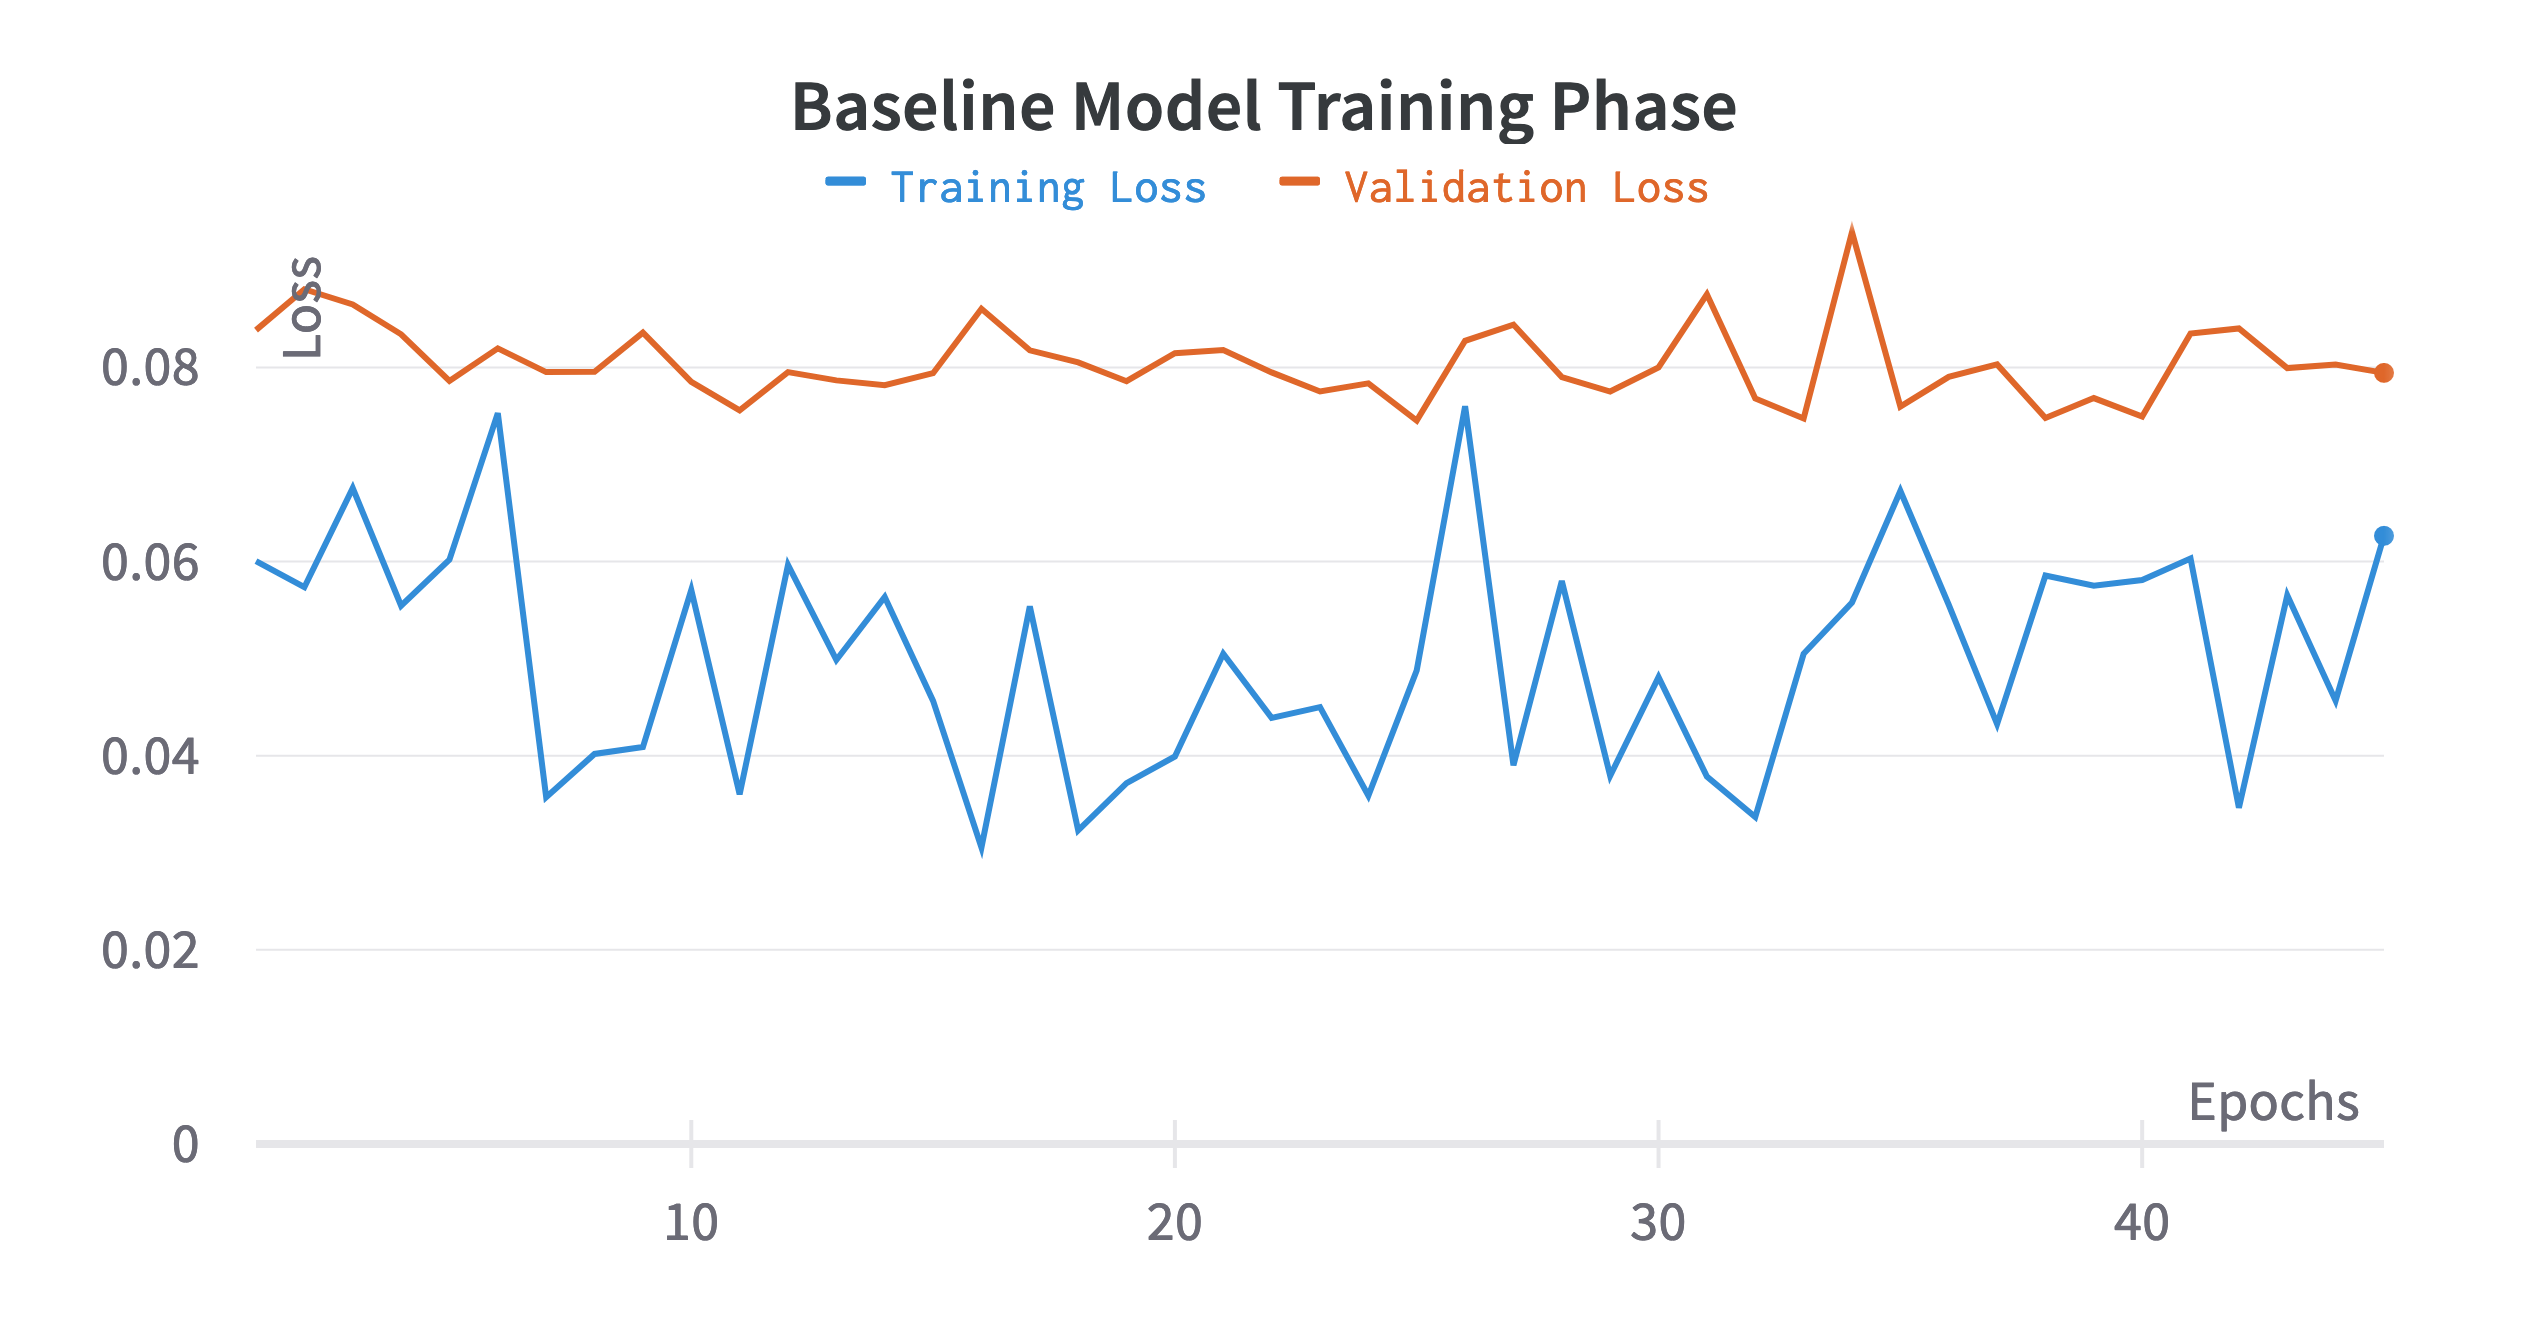
\includegraphics[width=\textwidth]{chapters/3_models/imgs/ufnc/ufnctraining.png}
	\caption{The chart displays the loss progression during the training phase. The blue line represents the Training Loss, while the orange line represents the Validation Loss.}
	\label{fig:ufcntraining}
\end{figure}

\begin{figure}[H]
	\centering
	\begin{subfigure}{0.32\textwidth}
		\centering
		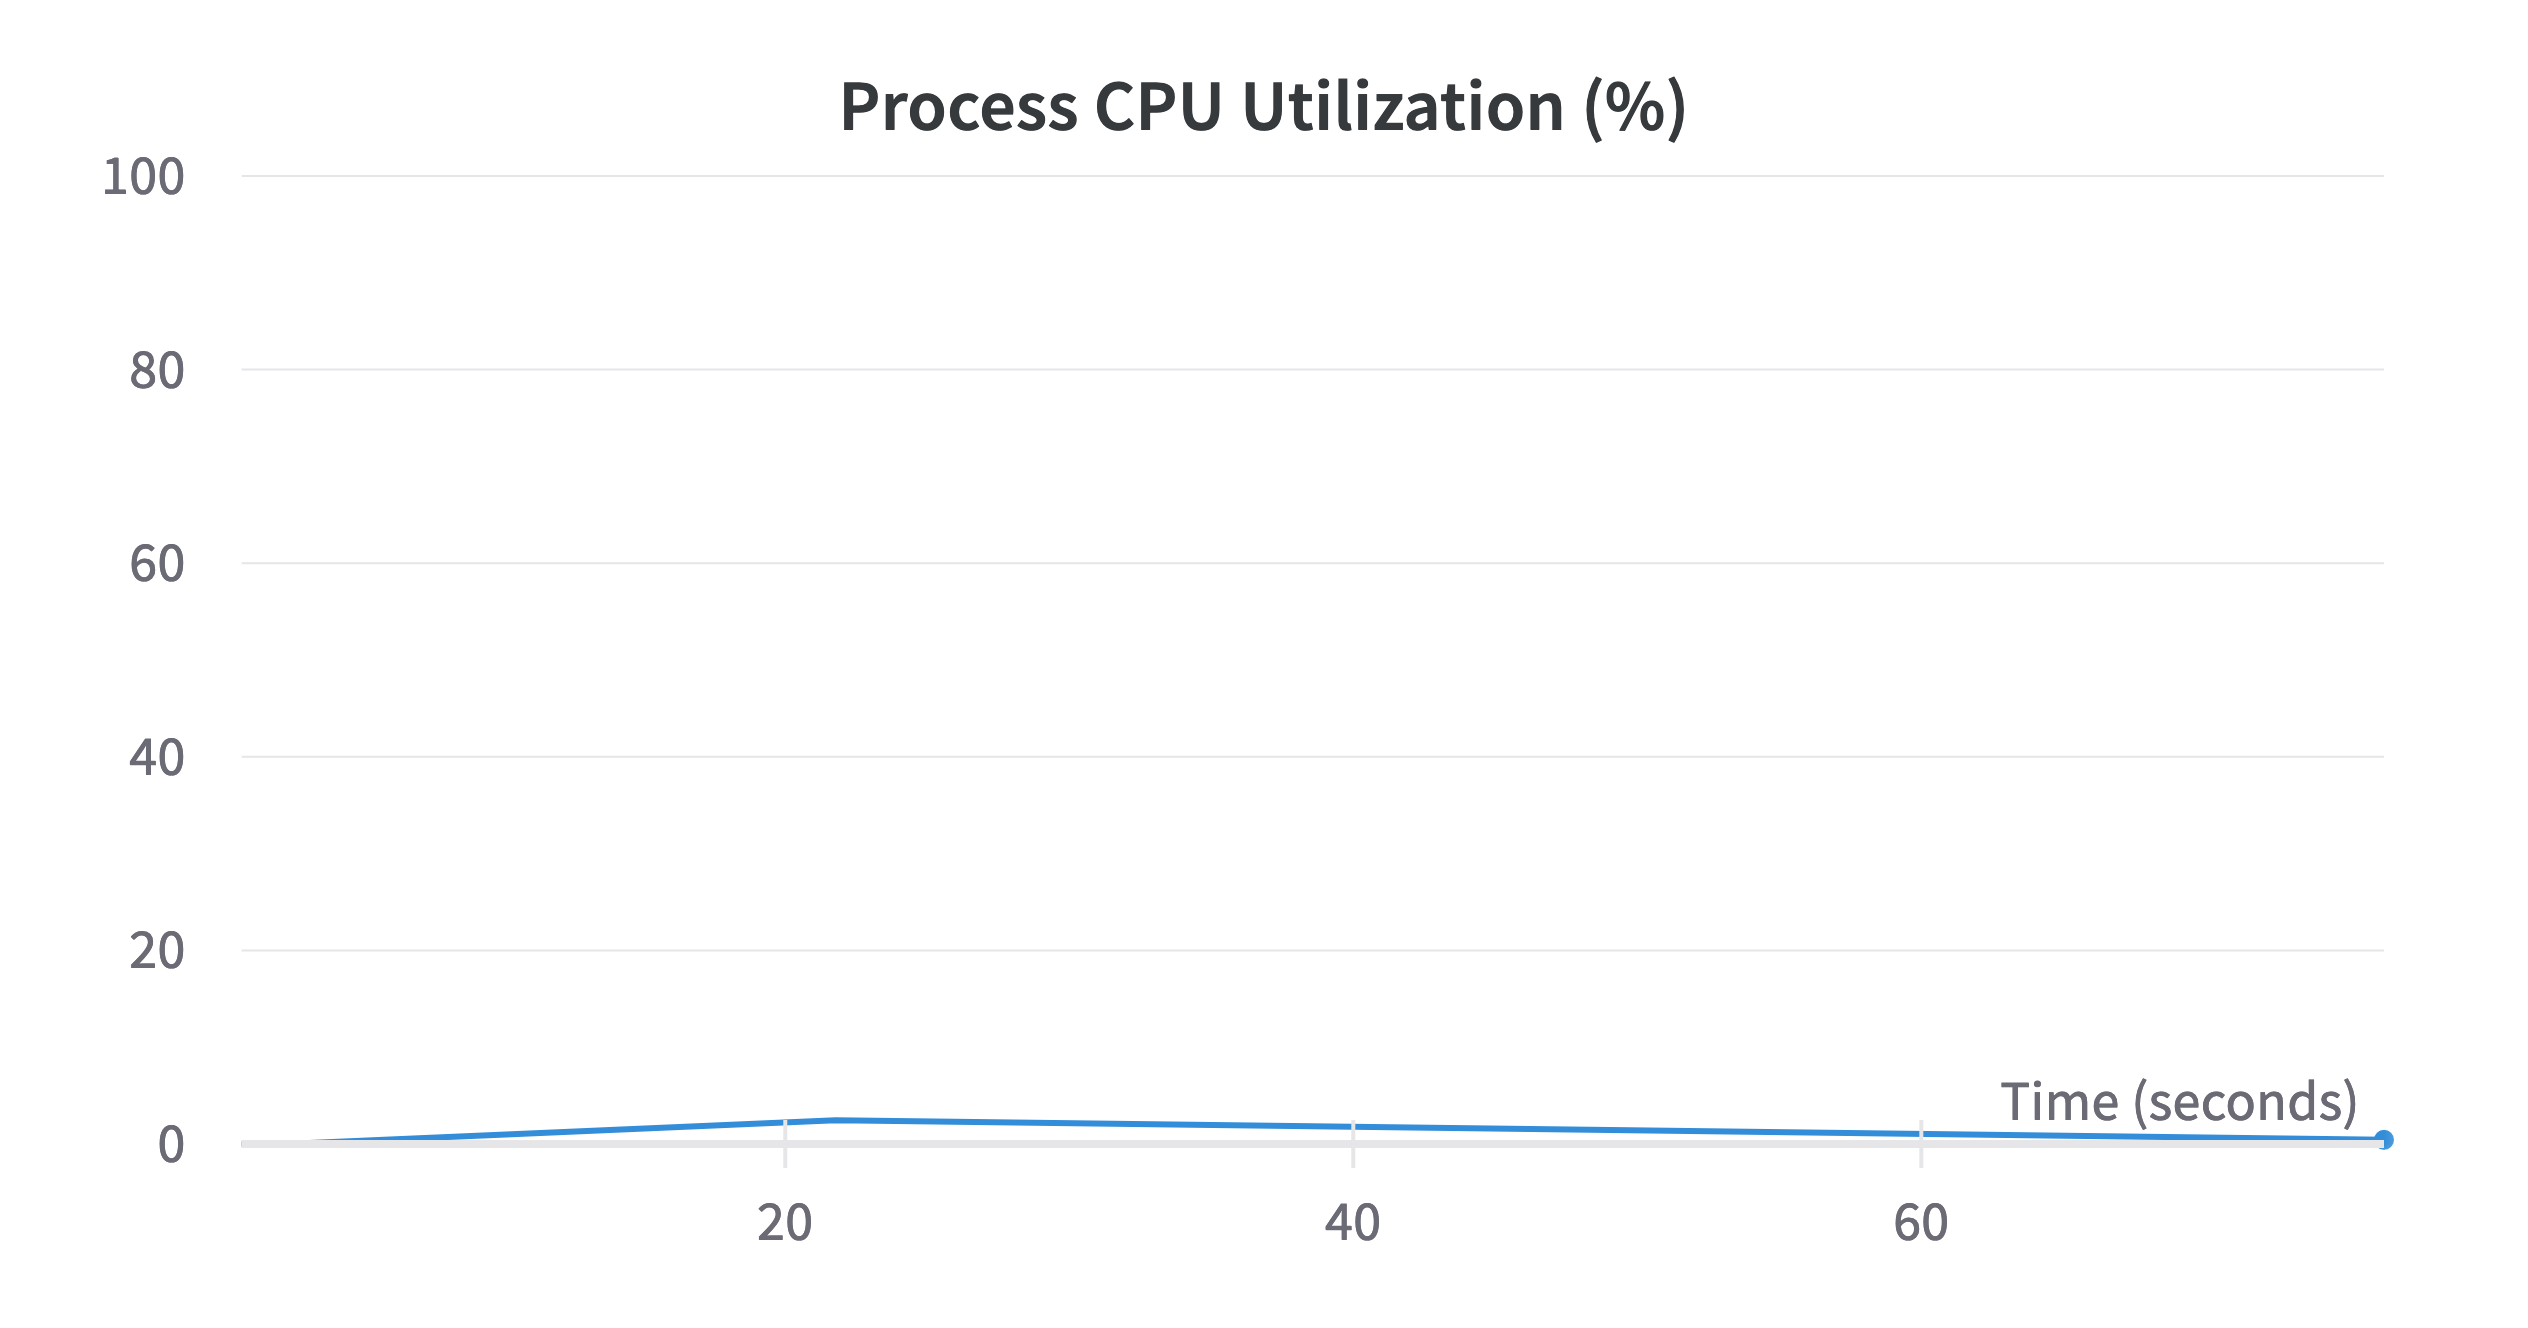
\includegraphics[width=\textwidth]{chapters/3_models/imgs/ufnc/ufcncpusage.png}
	\end{subfigure}
	\begin{subfigure}{0.32\textwidth}
		\centering
		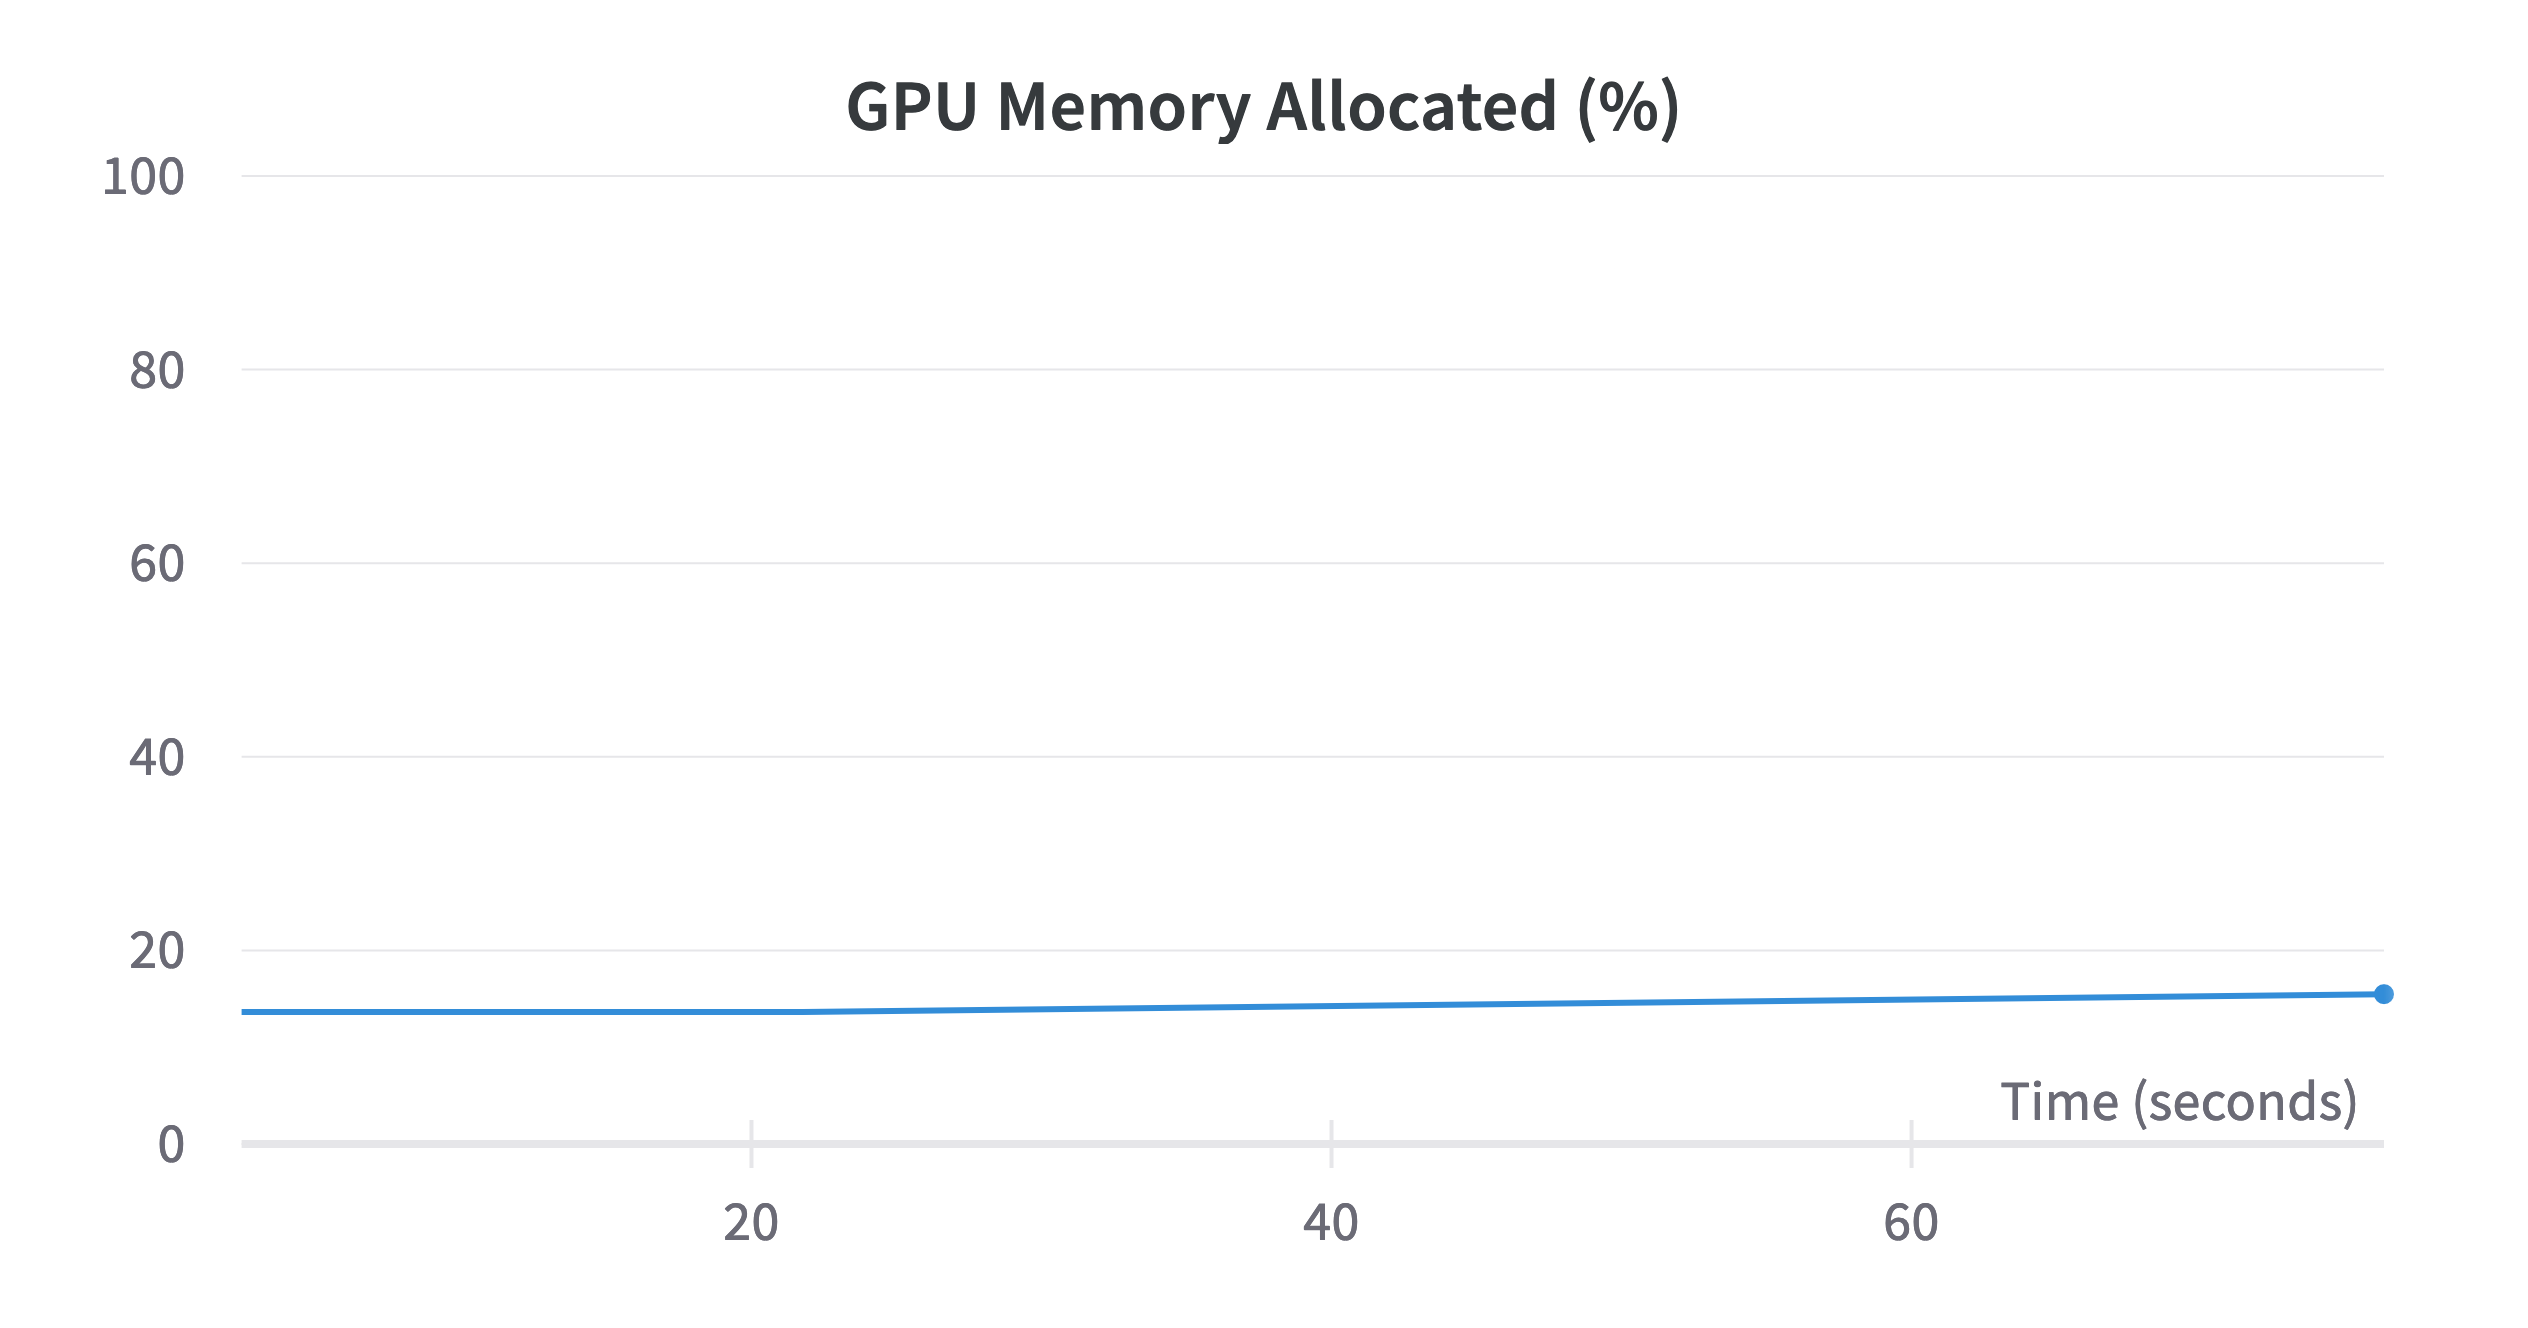
\includegraphics[width=\textwidth]{chapters/3_models/imgs/ufnc/ufcnmem.png}
	\end{subfigure}
	\begin{subfigure}{0.32\textwidth}
		\centering
		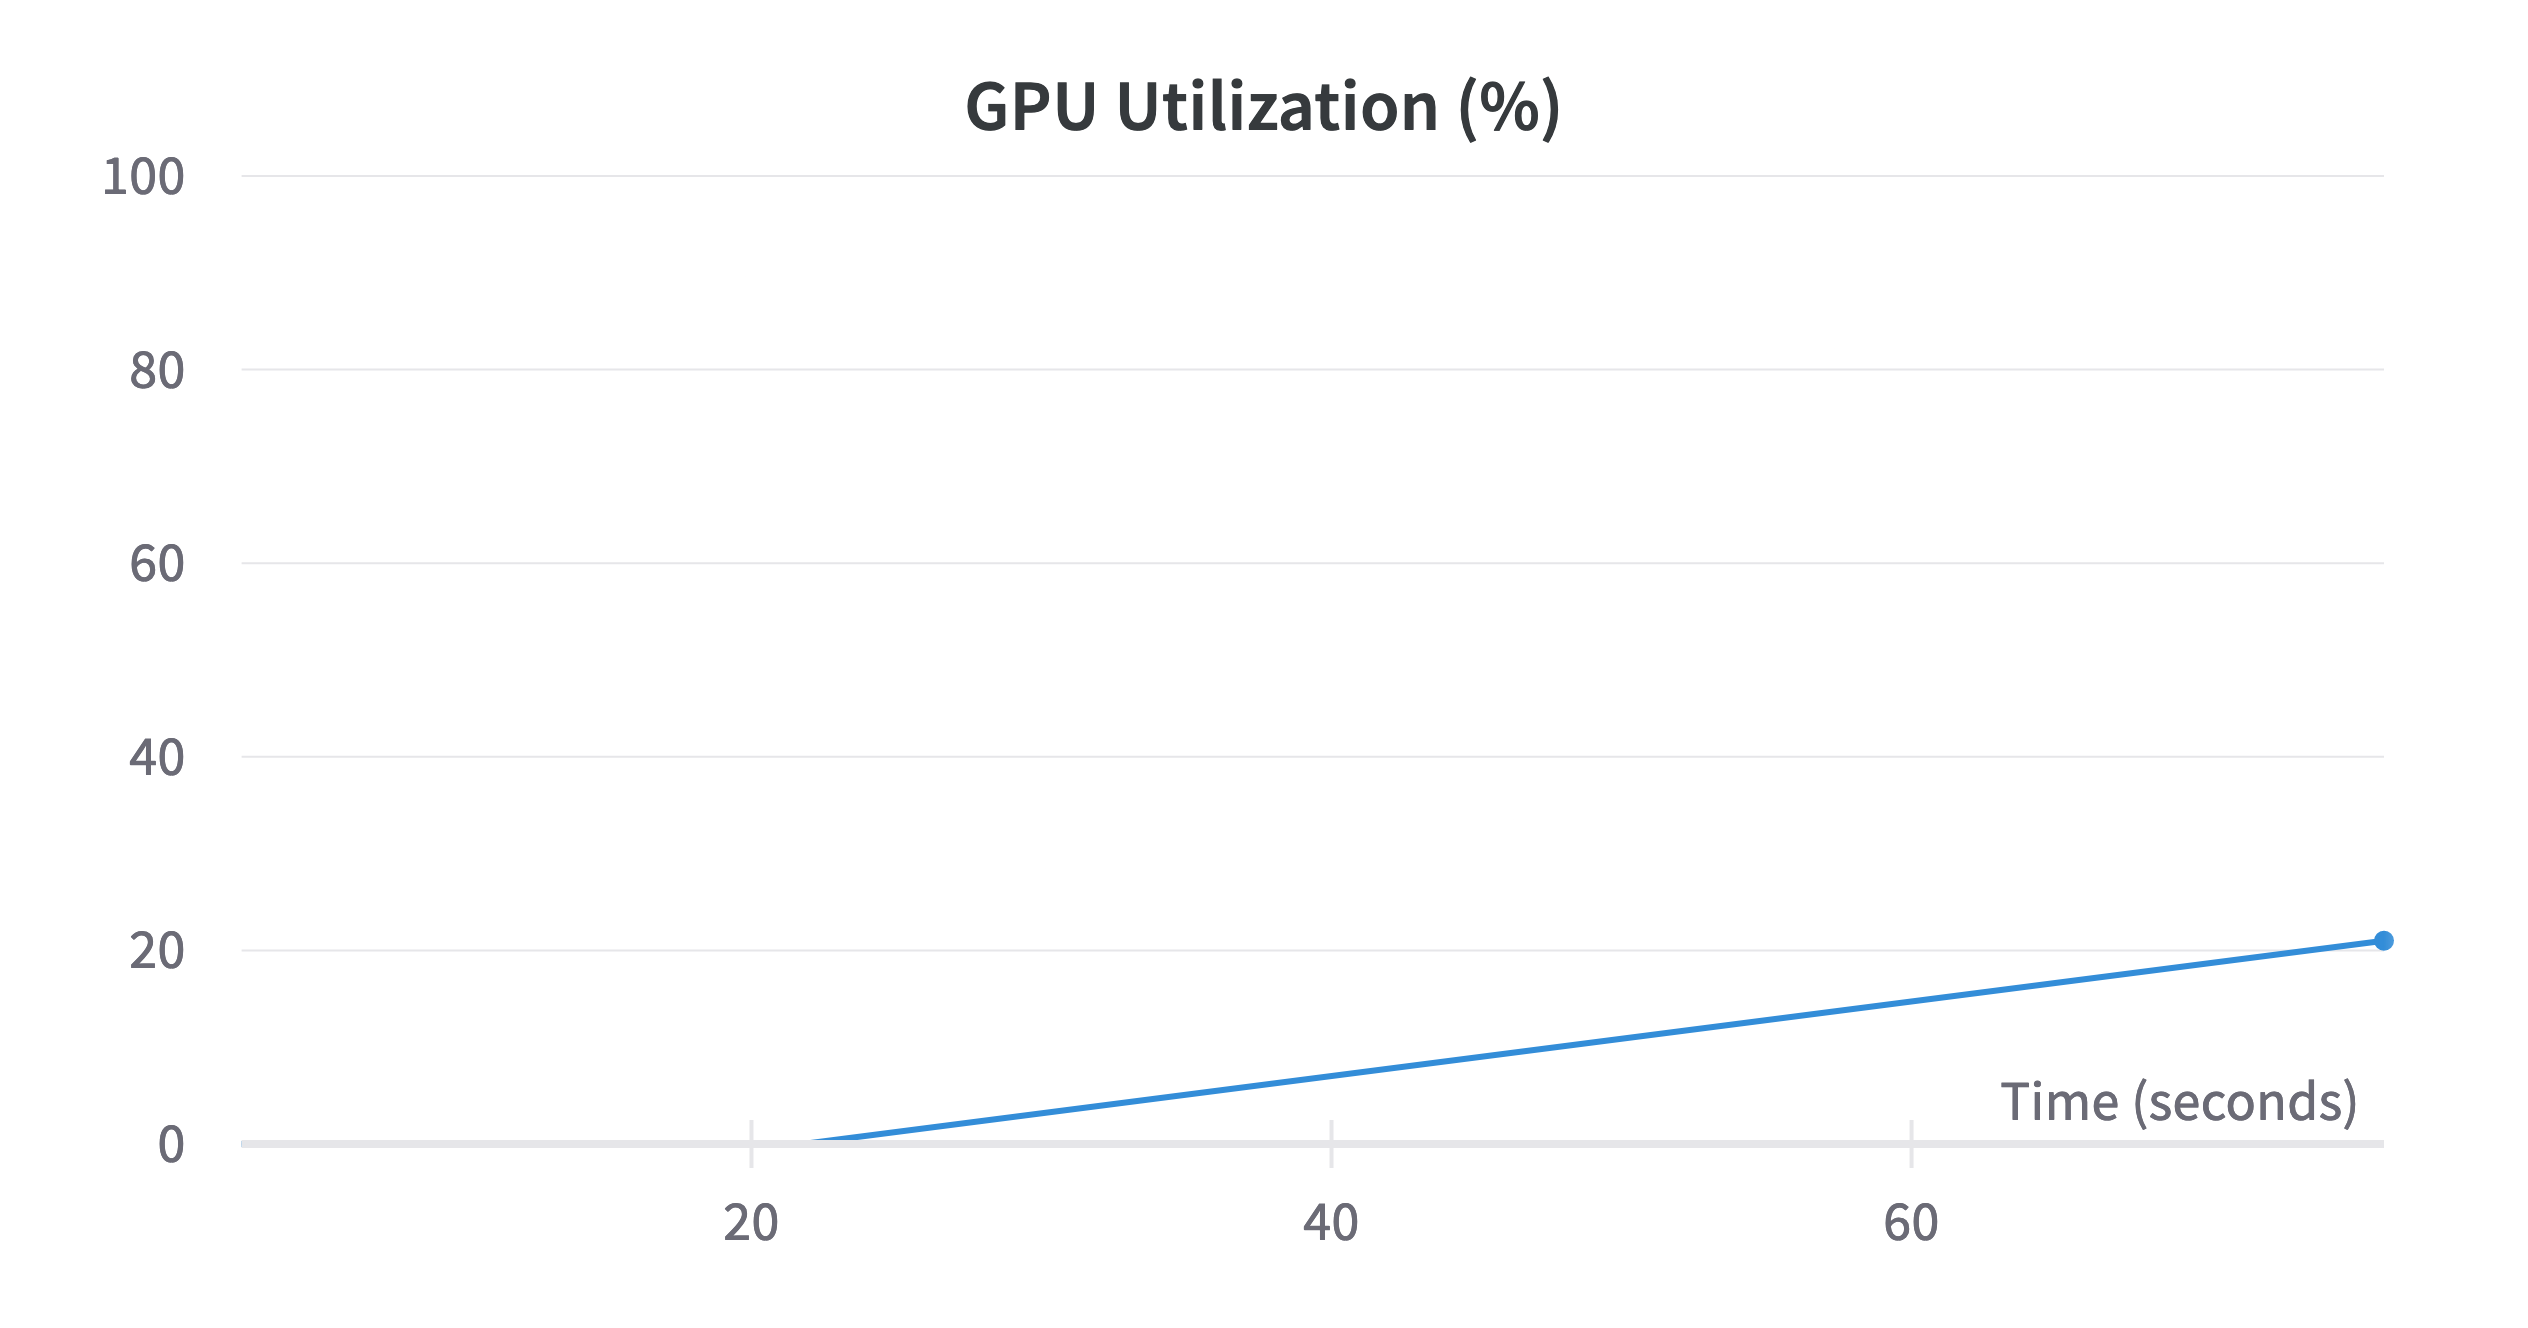
\includegraphics[width=\textwidth]{chapters/3_models/imgs/ufnc/ufcnusagevera.png}
	\end{subfigure}\\
	\begin{subfigure}{0.32\textwidth}
		\centering
		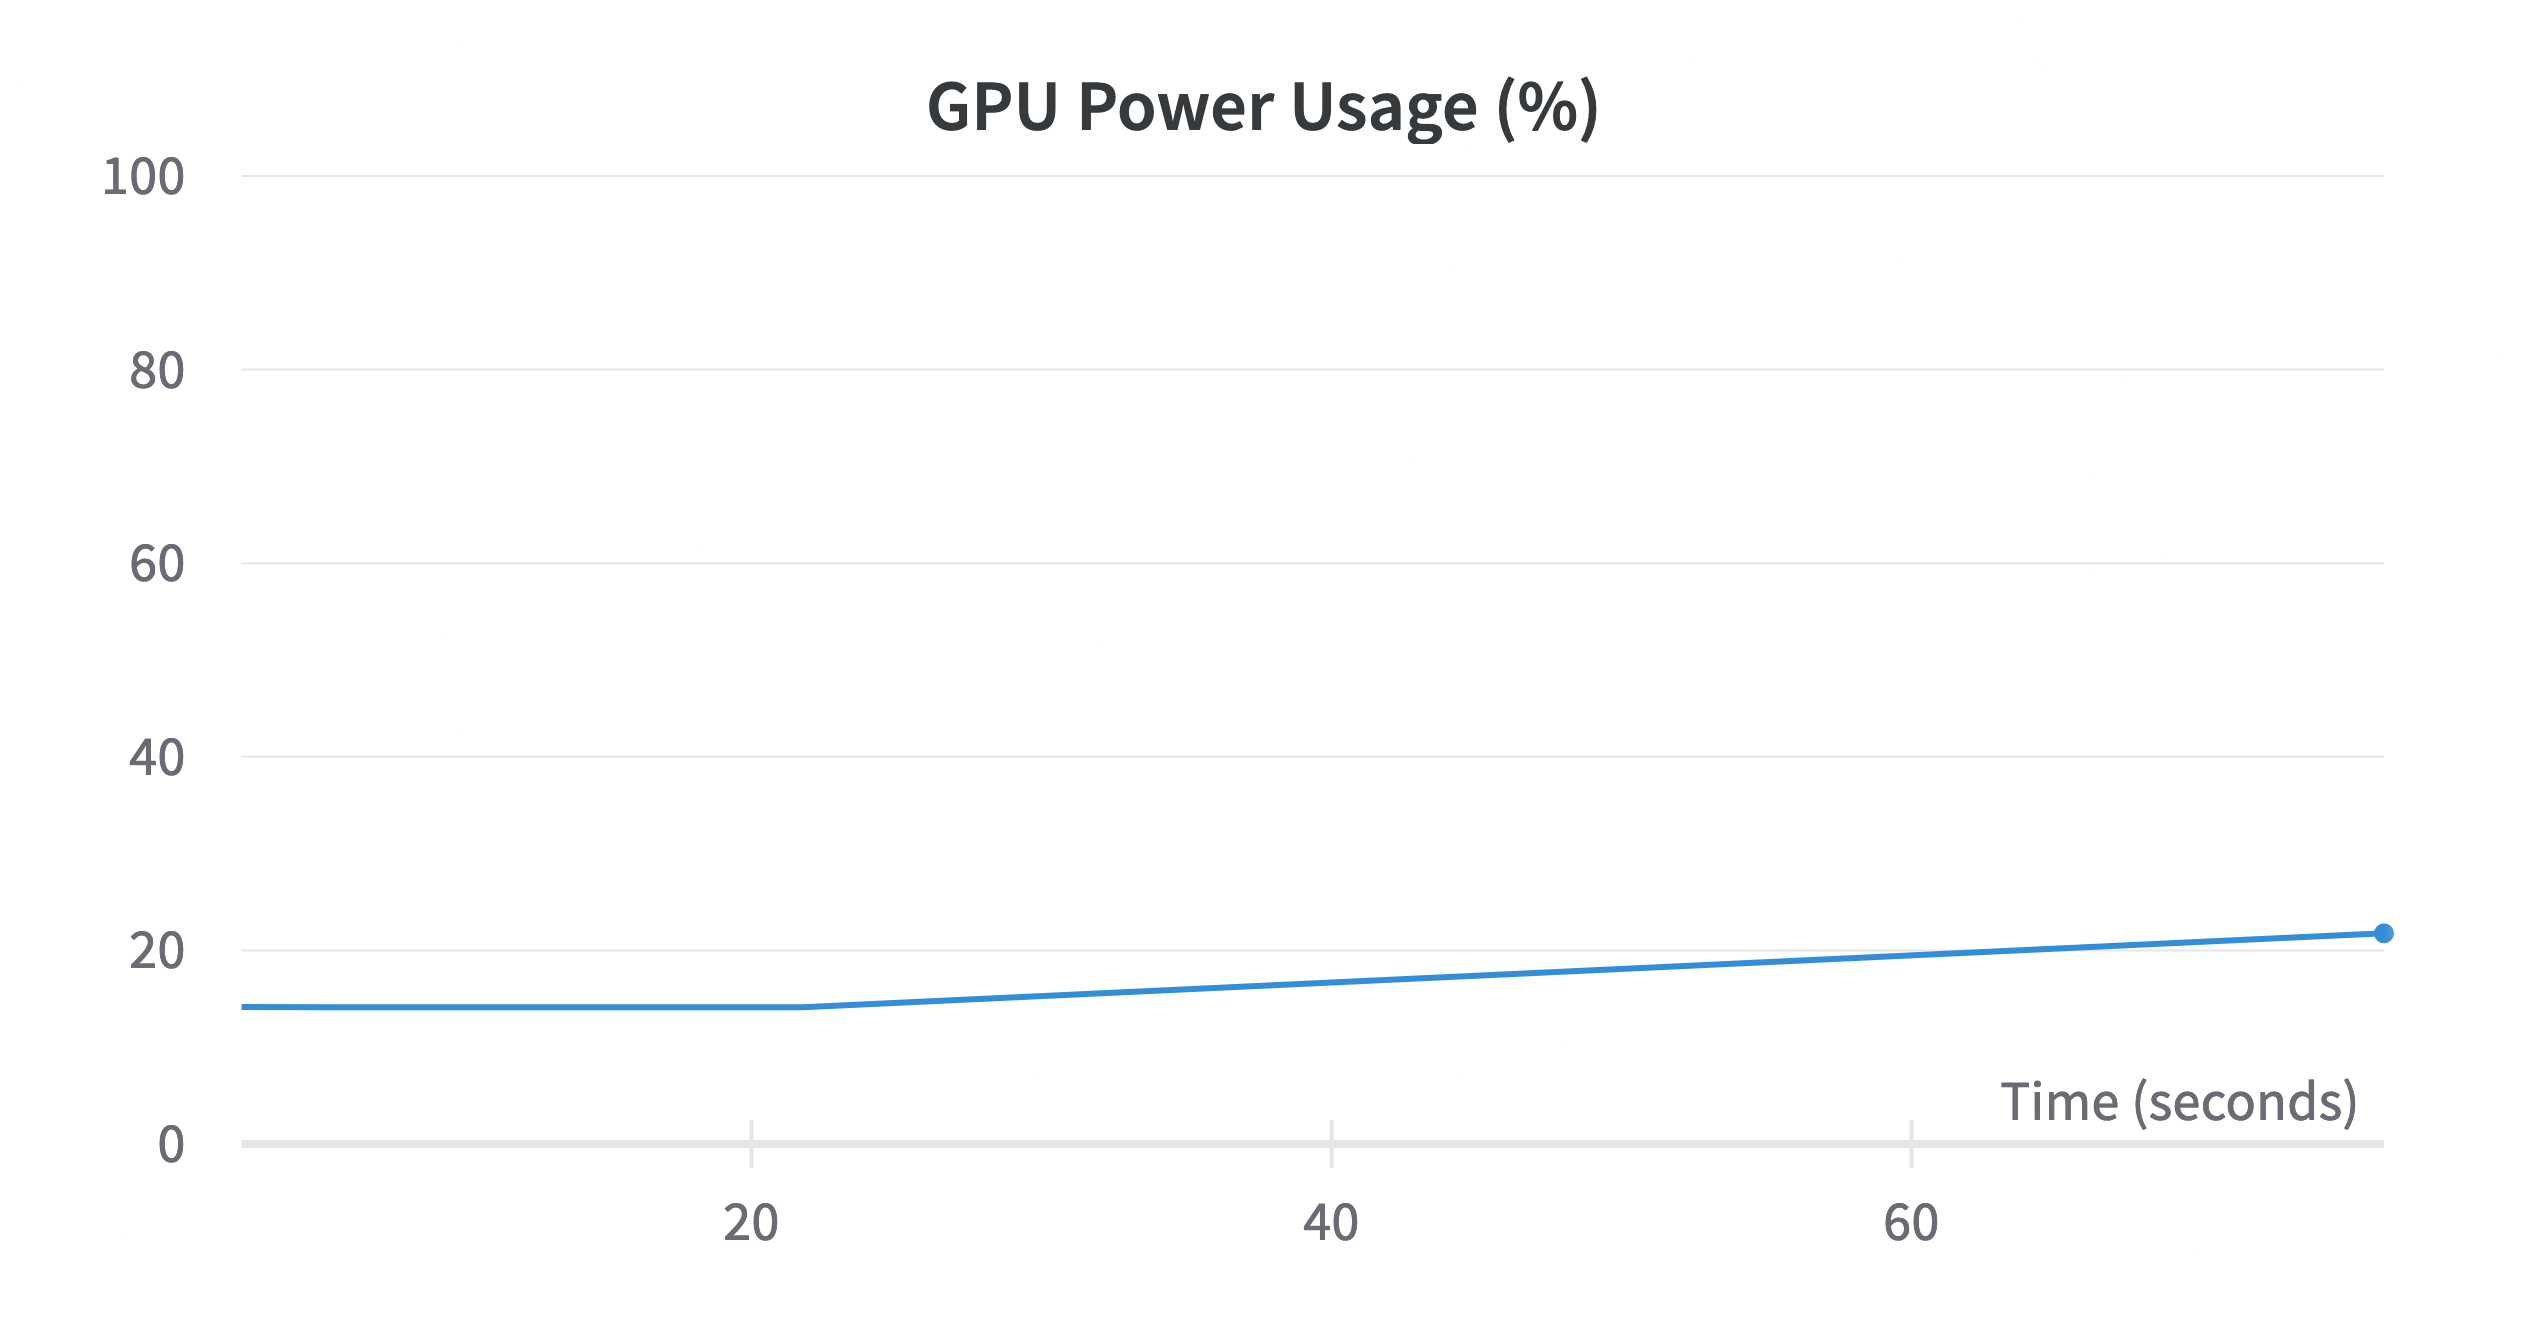
\includegraphics[width=\textwidth]{chapters/3_models/imgs/ufnc/ufncusageperc.png}
	\end{subfigure}
	\begin{subfigure}{0.32\textwidth}
		\centering
		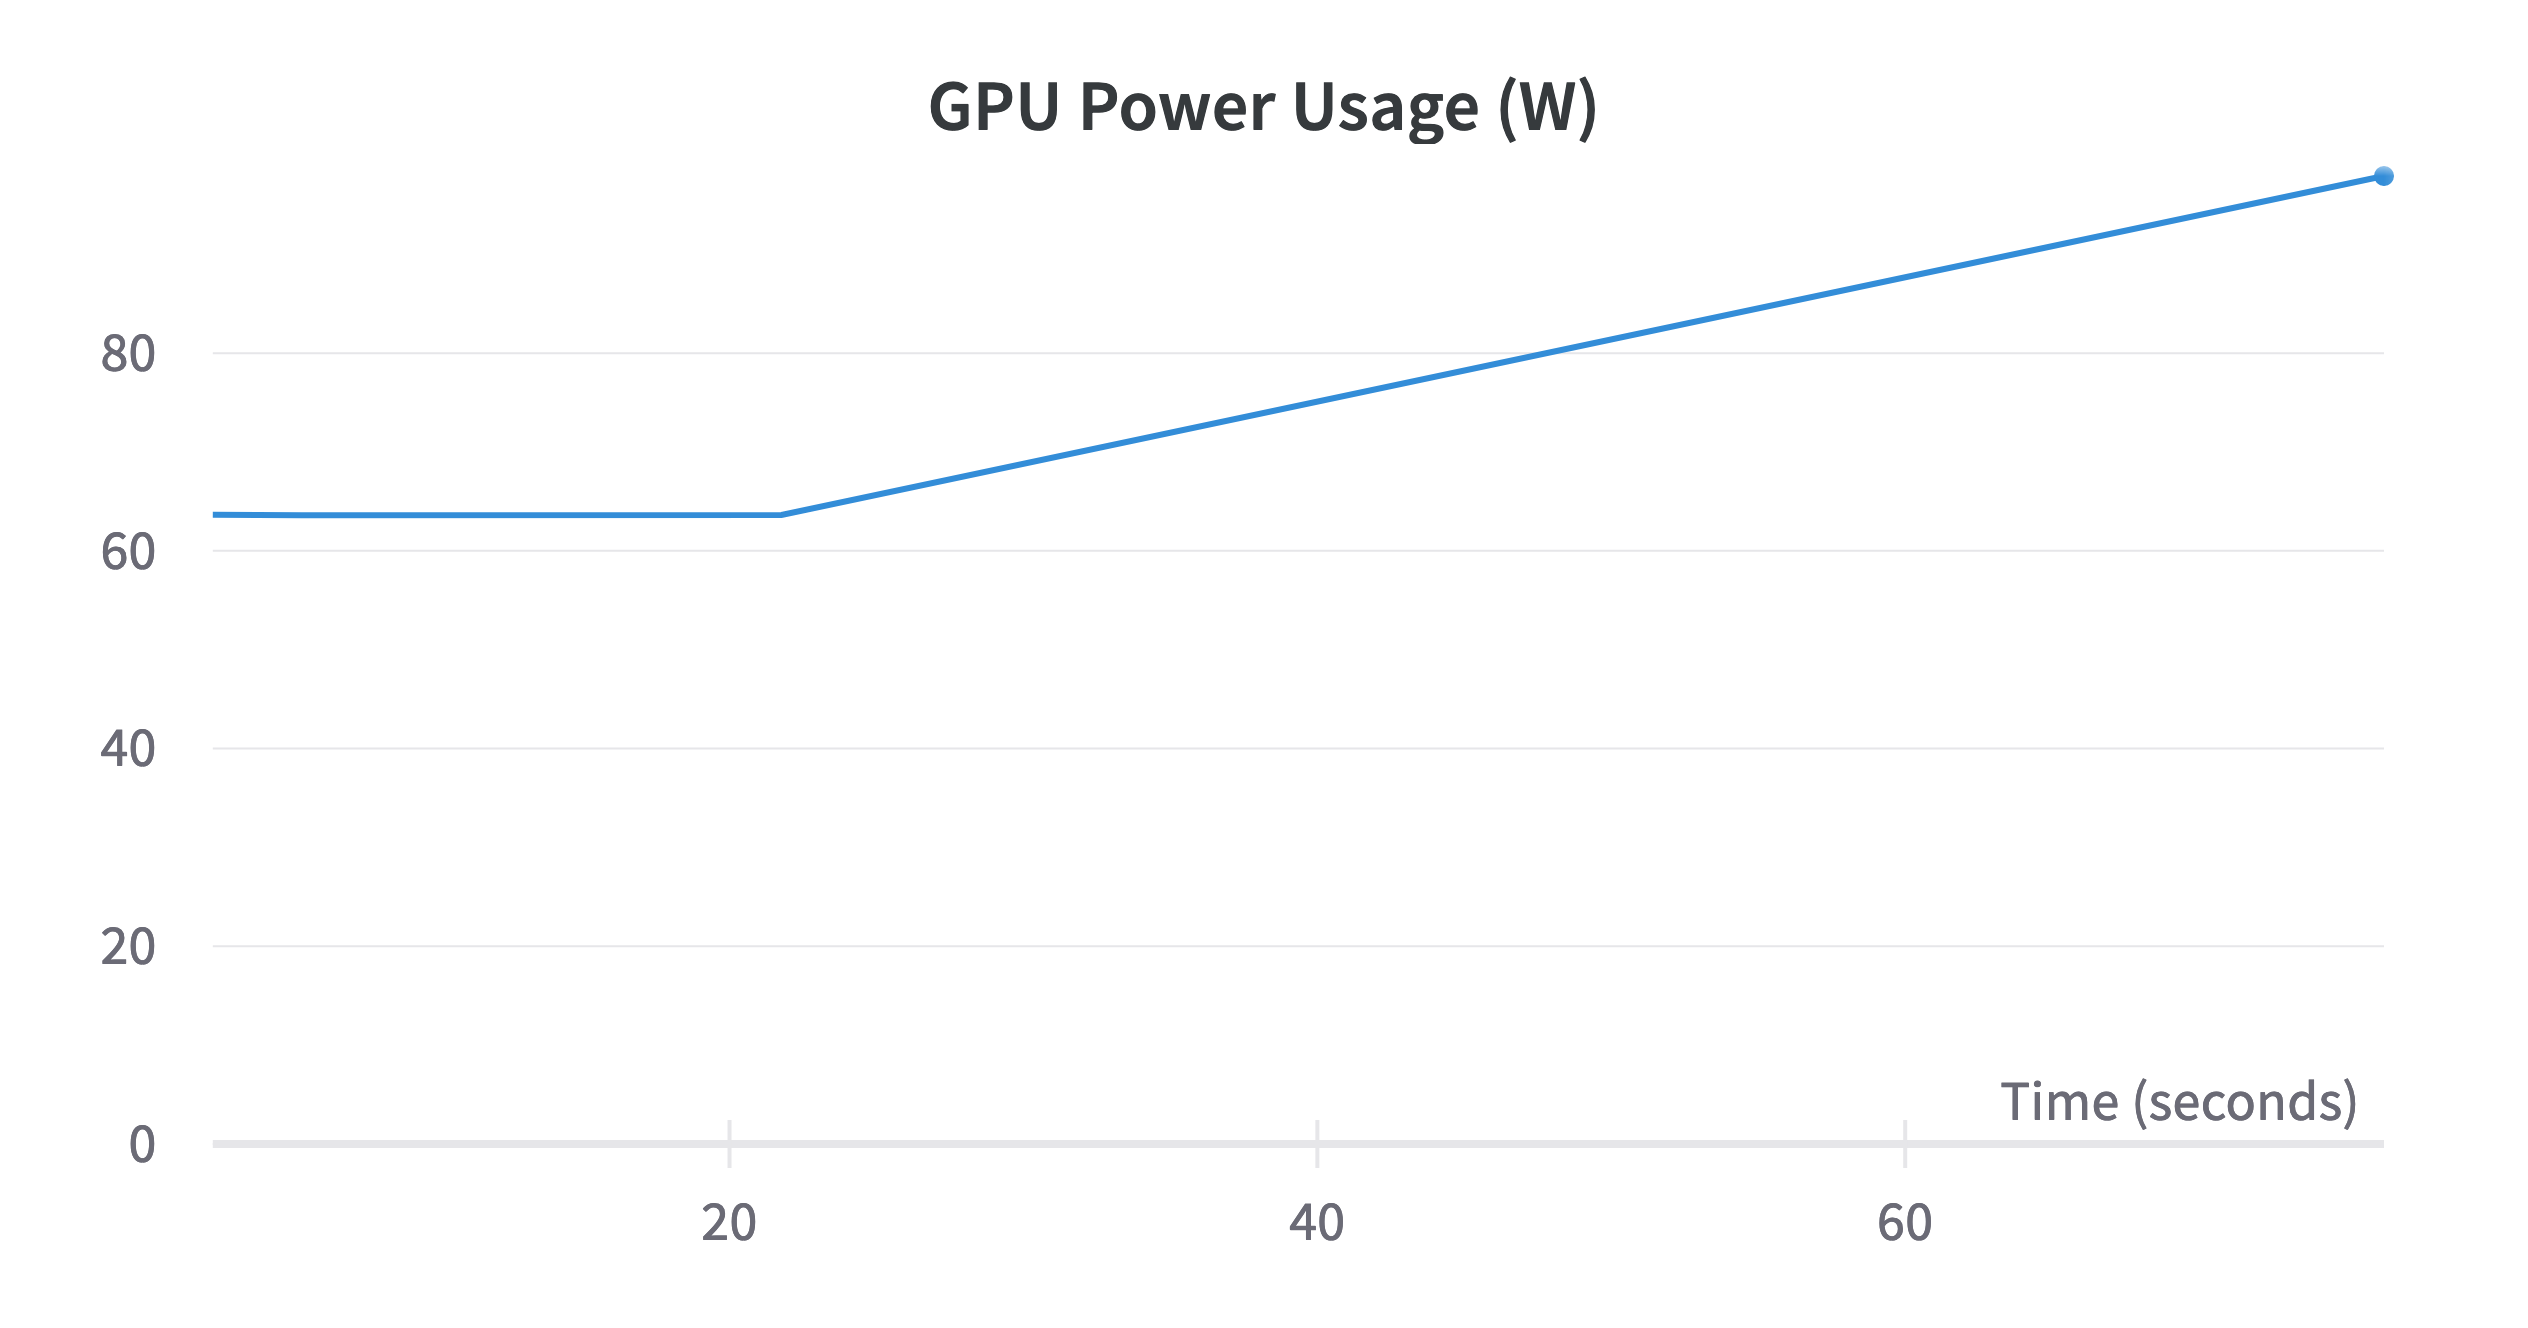
\includegraphics[width=\textwidth]{chapters/3_models/imgs/ufnc/ufncusagew.png}
	\end{subfigure}
	\begin{subfigure}{0.32\textwidth}
		\centering
		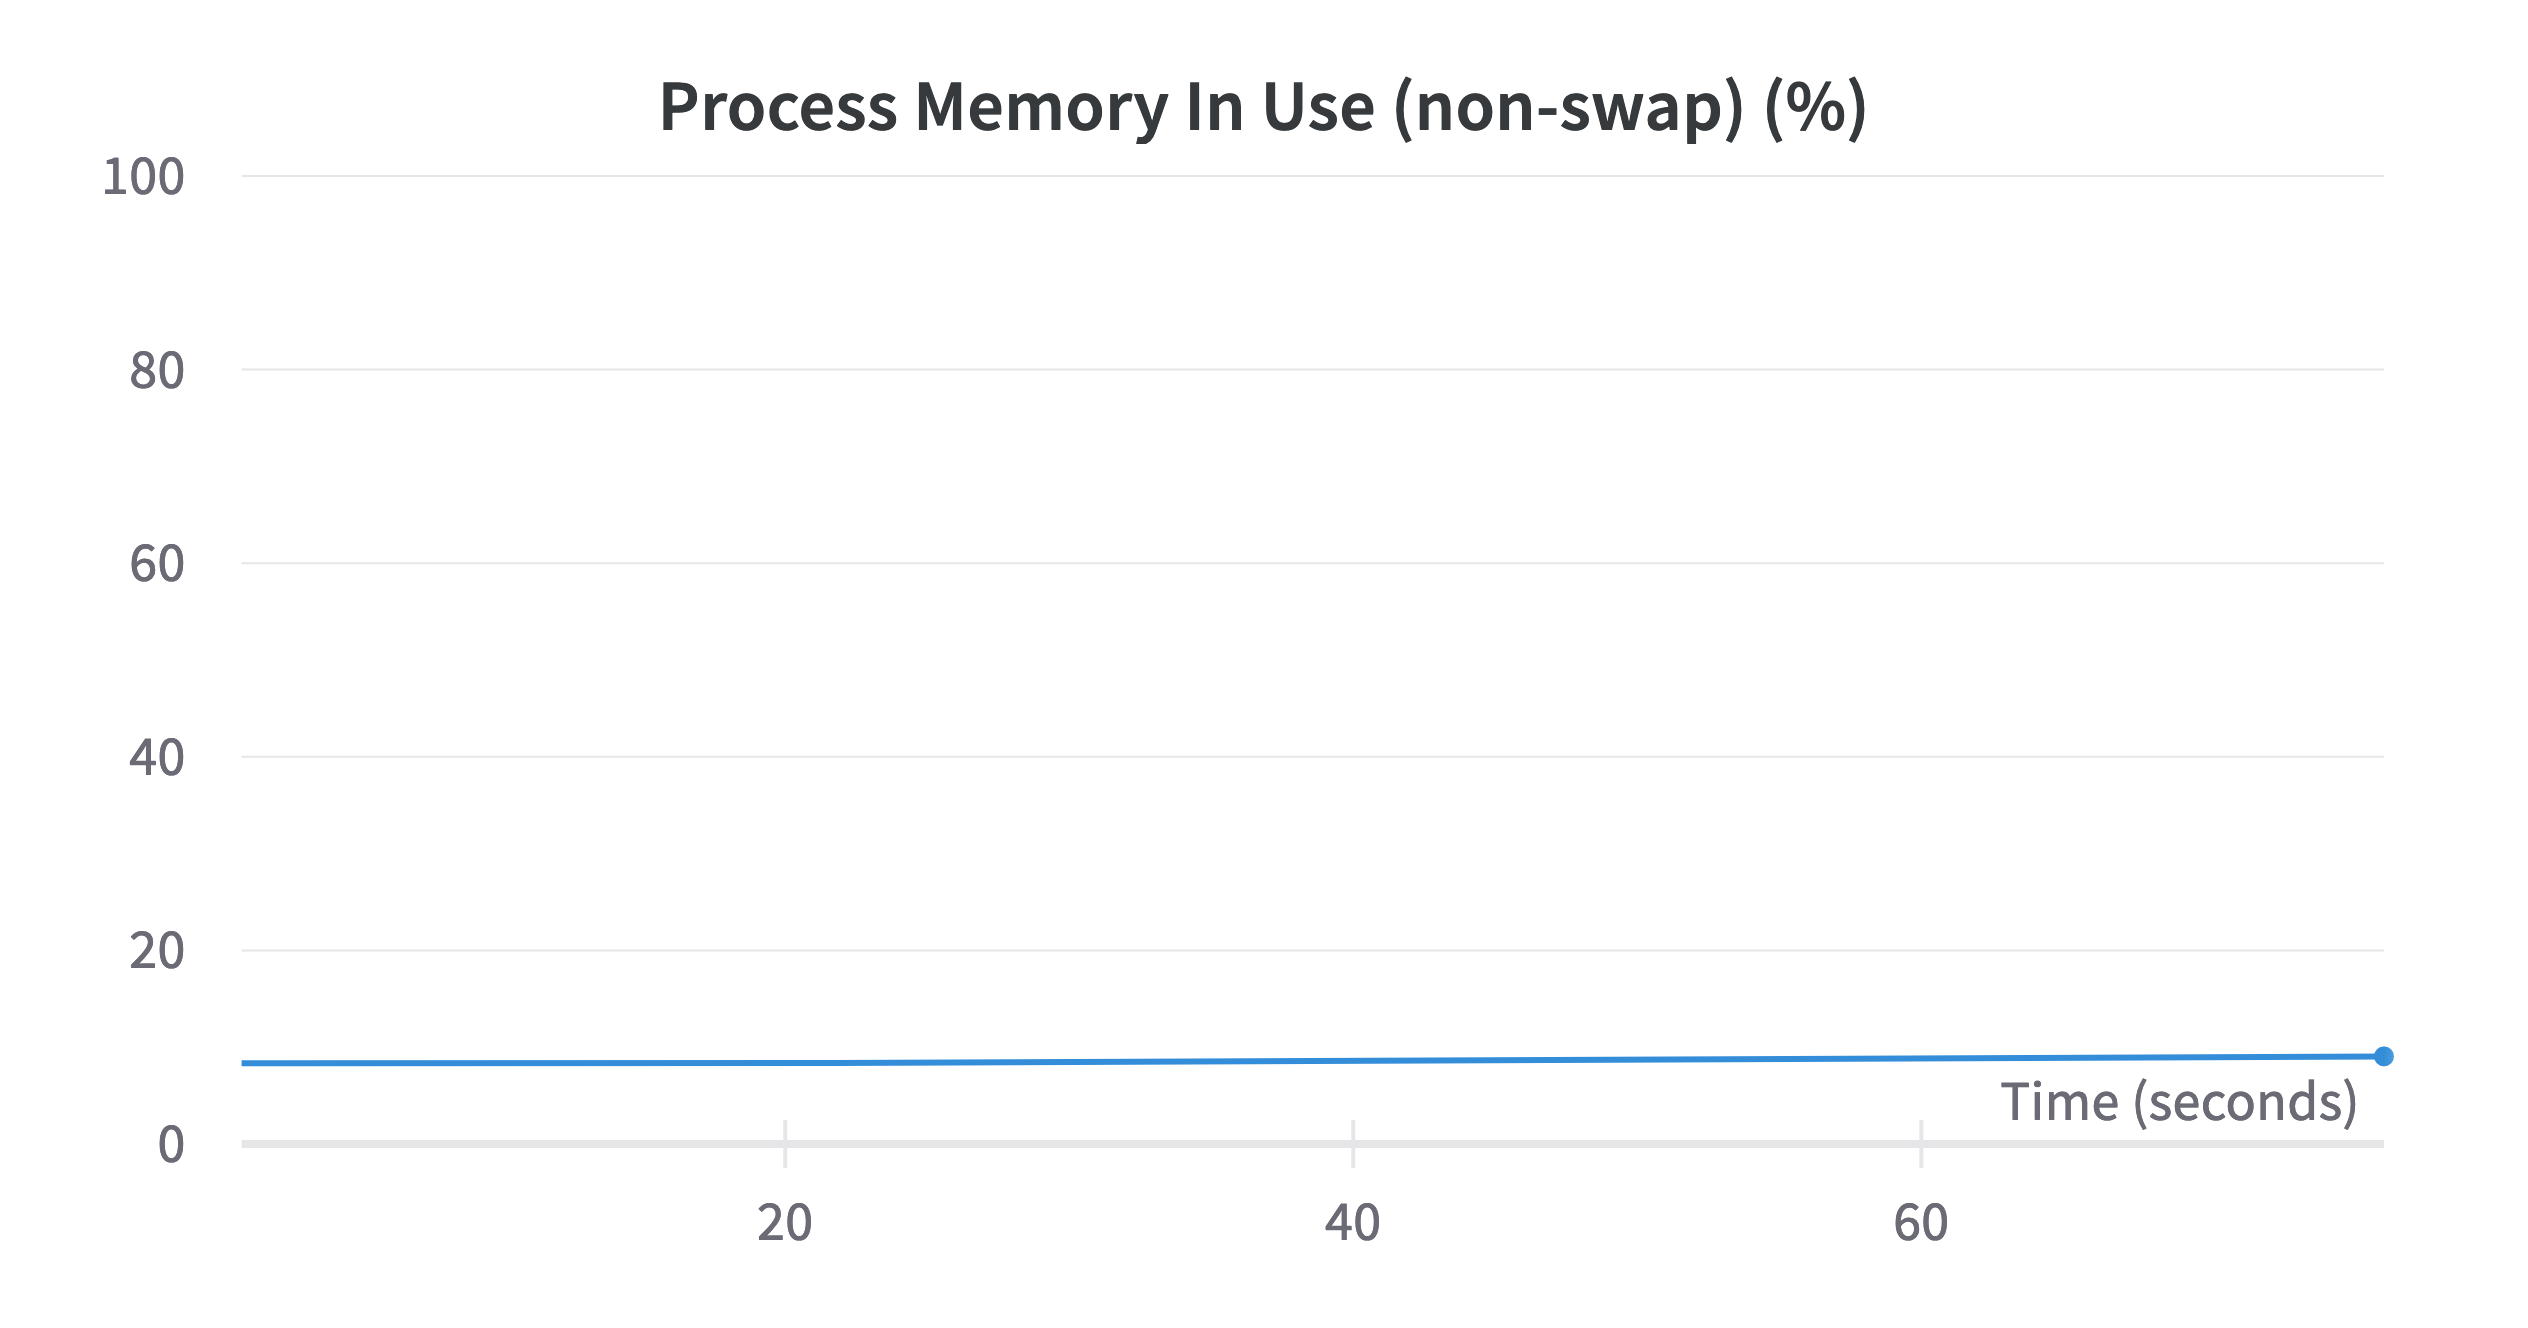
\includegraphics[width=\textwidth]{chapters/3_models/imgs/ufnc/ufcnmemram.png}
	\end{subfigure}\\
	\caption{System resources utilized during the Training phase.}
	\label{fig:ufcnsysusage}
\end{figure}

\begin{algorithm}[H]
	\caption{MLP model Training Algorithm}\label{alg:ufcntraining}
	\begin{algorithmic}
		\Require train/validation datasets; Baseline Neural Network Model

		\State Batch Size $\gets$ 10
		\State Learning Rate $\lambda \gets$ 0.01
		\State Epochs $\gets$ 100
		\State Patience $\gets$ 20
		\State loss $\gets$ L1Loss()
		\State Optimizer $\gets$ Adam Optimizer
		\State
		\For{\textbf{each} epoch \textbf{in} epochs}
		\For{\textbf{each} (batch\_id, before, after, target) \textbf{in} train.next\_batch()}

		\State train\_prediction $\gets$ model(before, after) \Comment{Model inference}
		\State train\_prediction $\gets \frac{\text{train\_prediction} \cdot \sum\text{train\_prediction}}{\sum target}$ \Comment{Area normalization}
		\State train\_loss $\gets$ loss(train\_prediction, target)
		\State Optimizer step
		\State Back Propagation
		\EndFor
		\State stop computing gradient
		\For{\textbf{each} (batch\_id, vbefore, vafter, vtarget) \textbf{in} validation.next\_batch()}
		\State val\_prediction $\gets$ model(vbefore, vafter) \Comment{Model inference}
		\State val\_prediction $\gets \frac{\text{val\_prediction} \cdot \sum\text{val\_prediction}}{\sum vtarget}$ \Comment{Area normalization}
		\State val\_loss $\gets$ loss(val\_prediction, vtarget)
		\EndFor

		\State check for Early Stopping
		\State check for Save Best Result
		\State start computing gradient
		\EndFor
	\end{algorithmic}
\end{algorithm}


\section{RNN}\label{sec:rnnbasemodel}
We will now introduce a second model based on Recurrent Neural Networks.
We will examine its structure, analyze the training phase,
and finally evaluate its performance, demonstrating how it manages
to outperform the previous architecture, the Baseline model introduced in Section~\ref{sec:mlpbaseline}.

%Andremo ora a presentare un secondo modello che si basa su Recurrent Neural Network. Vedremo la sua struttura, analizzeremo la
%fase di training ed infine valuteremo le sue performance e mostreremo come
%questo riuesce ad out-performare la precedente architettura, Baseline model, introdotta nella Sezione~\ref{sec:mlpbaseline}.

\subsection{Architecture}
This model is designed to make the most of the capabilities of
Recurrent Neural Networks to predict the behavior of instant
energy production during a variable-length gap period.

The required input format is similar to the previous one:
a tensor named \textit{before} containing the plant's status
one day before the gap, a tensor named \textit{after} with information
about the plant the day after the hole, and an additional tensor
named \textit{future} containing features that are \textit{always} available
even during blackout periods.
These features specifically include \verb|Solargis|, \verb|isday|,
and information obtained from OpenMeteo\cite{openmeteo}.
This last tensor should assist the model in prediction by helping
it better understand the state of meteorological conditions
and adapt instant production accordingly.

Now, let's display the main elements that compose it.

%Questo modello è pensato per sfruttare al meglio le potenzialità delle
%Reti Ricorrenti per riuscire a prevedere l'andamento dell'energia istantanea
%prodotta durante un periodo di buco a lunghezza variabile.
%
%La forma dell'input richiesta è simile a quella della precedente: un tensore chiamato \textit{before} contenente l'andamento dell'impianto un giorno prima del buco, un tensore chiamato \textit{after} con le informazioni dell'impianto del giorno dopo il buco ed in più un ultimo tensore chiamato
%\textit{future} che conterrà le feature che sono \textit{sempre} dispinibili anche durante i periodi di buco. Queste sono nello specifico: \verb|Solargis|, \verb|isday| e le informazioni reperite da OpenMeteo.
%Quest ultimo tensore dovrebbe aiutare il modello nella predizione permettendogli
%di capire meglio lo stato delle condizioni meteorologiche e di adeguare quindi la produzione istantanea.
%
%Mostriamo ora le parti principali che lo compongono:

\begin{itemize}
	\item \textbf{Input}: As described earlier, the model requires 3 input tensors: \textit{before}, \textit{after}, and \textit{future}. The first two should contain information from just one day before and after the gap, respectively, while the last one will have weather features to support predictions, which can vary in length. An example of input could be \verb|[BATCH_SIZE, 96, 33]| for \textit{before}, \verb|[BATCH_SIZE, 96, 33]| for \textit{after}, and \verb|[BATCH_SIZE, 288, 18]| for \textit{future}.
	      % come descritto in precedenza, il modello richiede 3 tensori in input: \textit{before}, \textit{after} e \textit{future}. I primi due dovranno contenere le informazioni di 
	      % uno ed un solo giorno prima e dopo il buco, mentre l'ultimo avrà le 
	      % feature meteo a supporto della predizione che potranno essere di lunghezza variabile. Un esempio di input può essere \verb|[BATCH_SIZE, 96, 33]| (before), \verb|[BATCH_SIZE, 96, 33]| (after) e \verb|[BATCH_SIZE, 288, 18]| (future).

	\item \textbf{Encoder}: This component's role is to identify the most important features described by the \textit{before} and \textit{after} tensors to understand how the plant is operating. These two tensors are passed to two different GRU\cite{gru2} layers, which will analyze these time series and extract key information. The final output of each GRU will then be extracted and concatenated together to form the Hidden State for the \textit{Decoder}.
	      % questo elemento ha il compito di andare
	      %  ad individuare le caratteristiche più importanti descritte dai
	      %  tensori \textit{before} e \textit{after} per poter capire quindi come
	      %  sta funzionando l'impianto. Questi due tensori vengono passati a due
	      %  layer GRU differenti che andranno ad analizzare queste serie temporali ed estrarranno le informazioni principali. Verrà quindi estrapolato l'ultimo output di ogni GRU per poi essere concatenate l'una dopo l'altra per formare l'Hidden State per il \textit{Decoder}.

	\item \textbf{Middle layer}: This layer consists of 2 Fully Connected Layers. It takes as input the result of the Encoding phase and reshapes it to the necessary format for input to the \textit{Decoder}. For both layers, the ReLU\cite{functions} function is used as the activation function.
	      %è formato da 2 Fully Connected Layers. Questo prende in input il risultato della fase di Encoding e lo riporta alla forma necessaria per essere passato
	      %in input al \textit{Decoder}. Per tutti e due i layer viene utilizzata
	      %la ReLu come funzione di attivazione.

	\item \textbf{Decoder}: Its role is to reprocess the information obtained from the Encoder and predict the instant energy produced during the blackout. It consists of a GRU layer that takes the \textit{future} tensor as input and uses the result of the Middle Layer as the hidden state.
	      % ha il compito di rielaborare le infromazioni
	      % ottenute dall'Encoder ed ottenere l'energia istantanea prodotta durante il buco. Questo è comopsta da un layer GRU che prende in
	      % input il tensore \textit{future} ed utilizza il risultato del
	      % Middle Layer come hidden state.

	\item \textbf{Output Layer}: This is the final layer of this architecture, and its task is to transform the output from the Decoder into a tensor of shape \verb|[Batch_Size,| \verb|Gap_Len,| \verb|1]|, representing the instant energy produced by the plant during the gap. It consists of a Fully Connected Layer. Its output is then multiplied by the feature \verb|isday| to ensure that the model's prediction is always zero during the night.
	      % è l'ultimo livello di questa
	      % architettura e ha il compito di trasformare l'output del Decoder
	      % in un tensore di forma \verb|[Batch_Size, Gap_Len, 1]| che rappresneta
	      % l'energia istantanea prodotta dall'impianto durante il buco.
	      % \'{E} formato da un Fully Connected Layer.
	      % Il suo output viene poi moltiplicato per la feature \verb|isday|
	      % così da assicurarci che la predizione del modello durante
	      % la notte sia sempre nulla.
\end{itemize}

\begin{figure}[H]
	\centering
	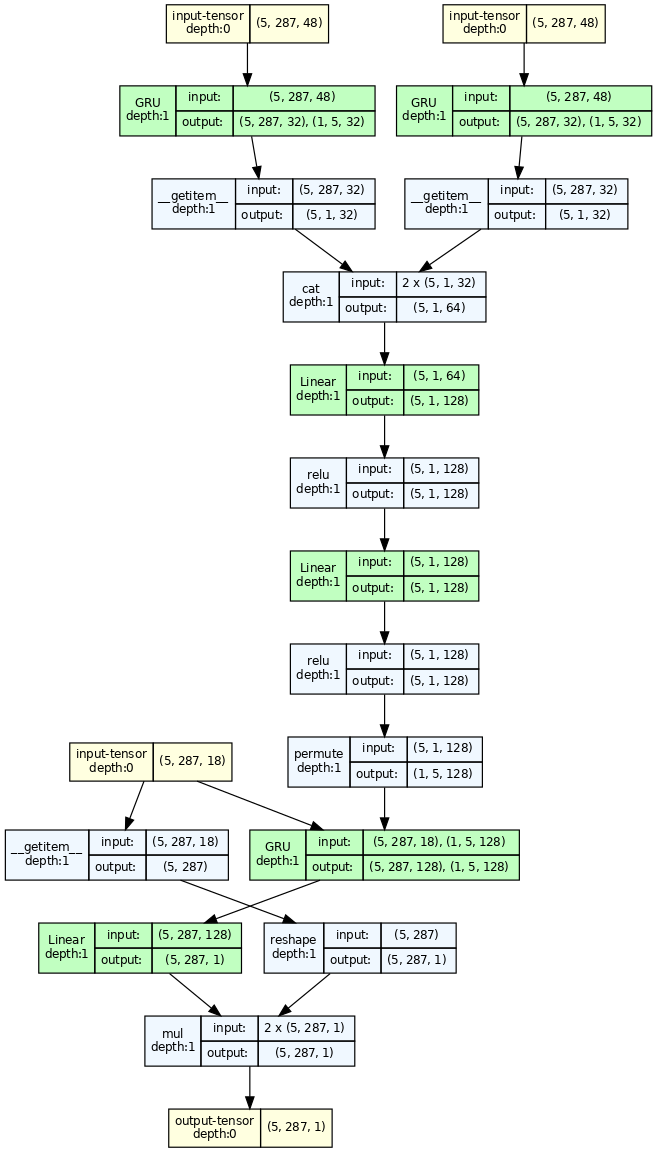
\includegraphics[height=.9\textheight]{chapters/3_models/imgs/grrun/grrunarchitecture.png}
	\caption{Recurren Neural Netowrk Based Model architecture visualization.}\label{fig:grrunarchitecture}
\end{figure}

\subsection{Training}
The model was trained to learn the trend of the instant energy production curve of
the plant during gaps of variable lengths, ranging from a minimum of 1
day to a maximum of 4 days.
These gaps were artificially generated in the training dataset and provided to the model
as described earlier, with attention to grouping gaps of the same length in
batches to avoid complications during training.

In this case, an \textit{Early Stopping}\cite{es} and \textit{Save Best} procedure were implemented
as well to ensure that the model always saves the best-performing model and to prevent
resource waste.

The validation dataset was applied in this phase to conduct an initial
and preliminary evaluation of the training process and highlight potential issues.
A normalization procedure was also applied to scale the prediction area with respect
to the ground truth area.
This allows the model to learn the shape of the curve and not exceed the limits
of energy production during the gap.

The Adam\cite{adam} optimizer was used, and the L1Loss\cite{loss} was applied as the loss function.
The batch size was set to 10, the learning rate ($\lambda$) was set to 0.01,
a maximum of 100 epochs was set, and the patience was set to 20.

%Il modello è stato allenato per cercare di apprendere l'andamento della
%curva dell'energia istantanea prodotta dall'impianto durante buchi di 
%dimensione variabile che vanno da un minimo di 1 giorno ad un massimo di 4 giorni. Questi buchi sono stati generati artificialmente nel dataset di training e passati al modello come descritto in precedenza
%facendo attenzione a raggruppare in batch sempre buchi della stessa 
%dimensione per evitare complicazioni durante l'addestramento.
%Anche qui è stata implementata una procedura di \textit{Early Stopping} e \textit{Save Best}
%per garantire sempre di salvare il modello con le prestazioni migliori
%ed evitare spreco di risorse.
%Il dataset di validation è stato applicato in questa fase per poter
%effettuare una prima e sommaria valutazione della procedua di addestramento ed evidenziare potenziali problemi.
%Anche in questo caso è stata applicata una procedura di normalizzazione 
%dell'area della predizione rispetto a quella della ground thorught per
%far si che il modello apprenda a predirre la forma della curva e che non
%superi i limiti di energia prodotta durante il buco.
%L'ottimizzatore Adam è stato impiegato ed è stata applicata la L1Loss come loss function.
%Abbiamo impostato a 10 la batch size, a 0.01 il learning rate $\lambda$, un
%massimo di 100 epoche ed una patience pari a 20.

\begin{table}[H]
	\begin{center}
		\begin{tabular}[c]{l|l}
			\textbf{Total Parameters (\#)}     & 92737 \\
			\textbf{Trainable Parameters (\#)} & 92737 \\
			\textbf{Training Duration (s)}     & 39.0  \\
			\textbf{Model Size (KB)}           & 366.6
		\end{tabular}
	\end{center}
	\caption{RNN based model specification.}\label{tab:ufcnspecs}
\end{table}

\begin{figure}[H]
	\centering
	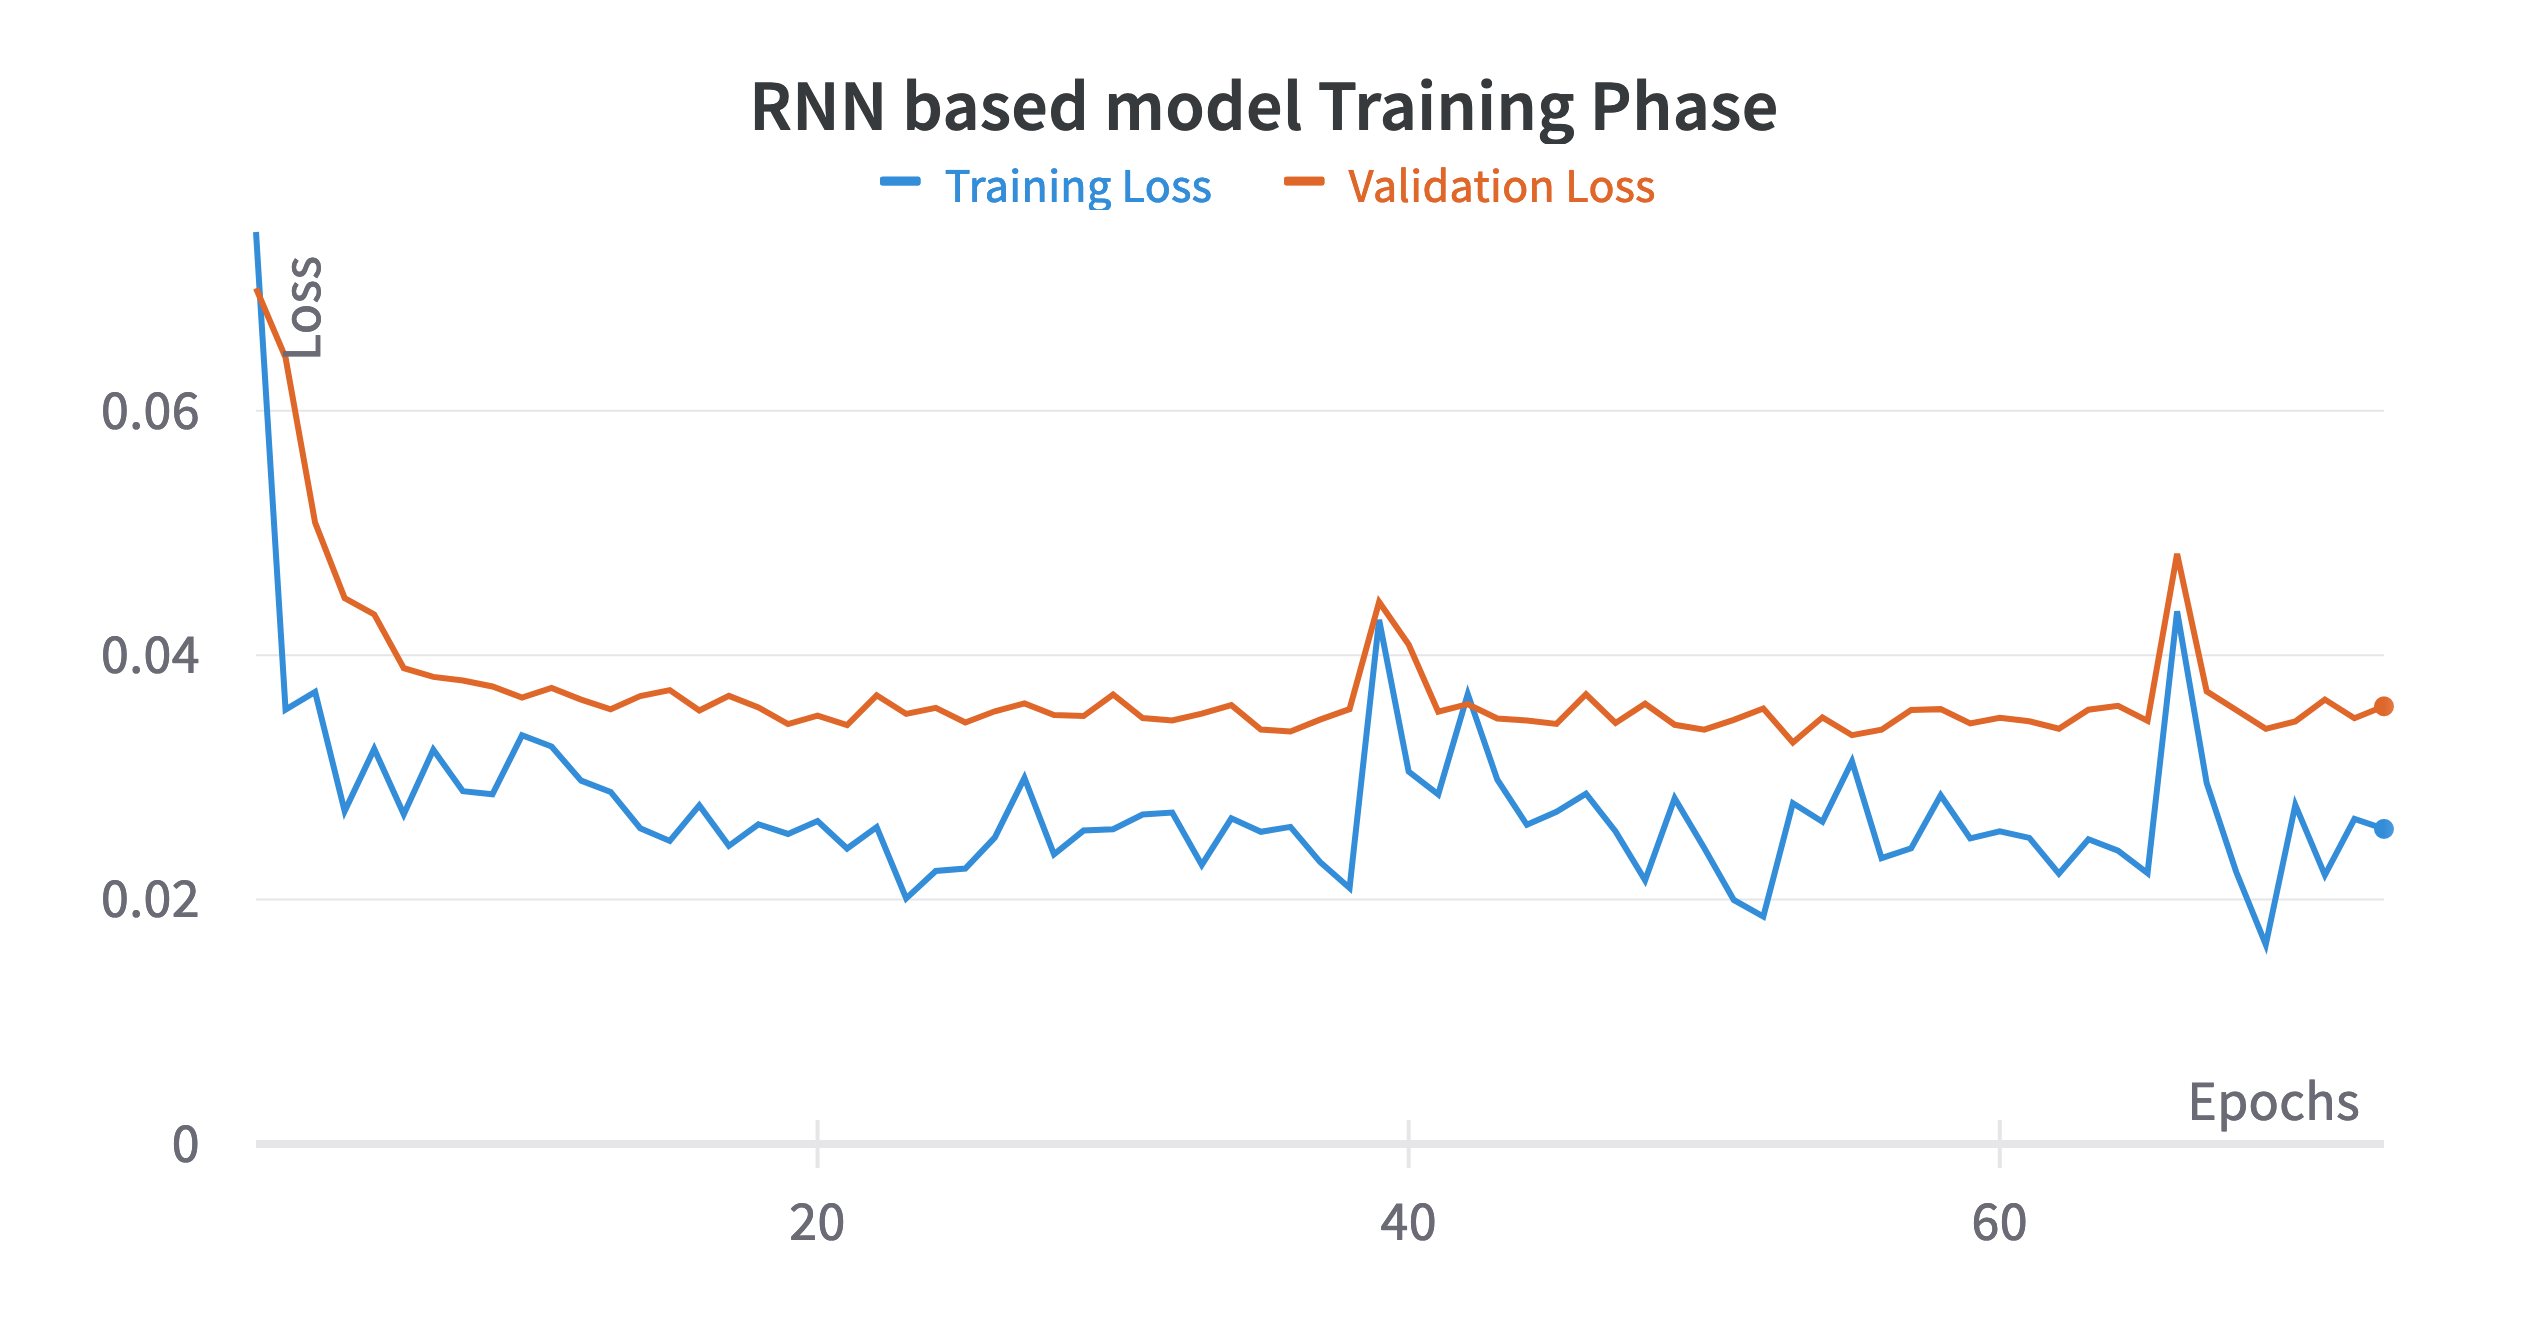
\includegraphics[width=.8\linewidth]{chapters/3_models/imgs/grrun/grruntraining.png}
	\caption{The chart displays the loss progression during the training phase.The blue line represents the Training Loss, while the orange line represents the Validation Loss.}
	\label{fig:grruntraining}
\end{figure}

\begin{figure}[H]
	\centering
	\begin{subfigure}{0.43\textwidth}
		\centering
		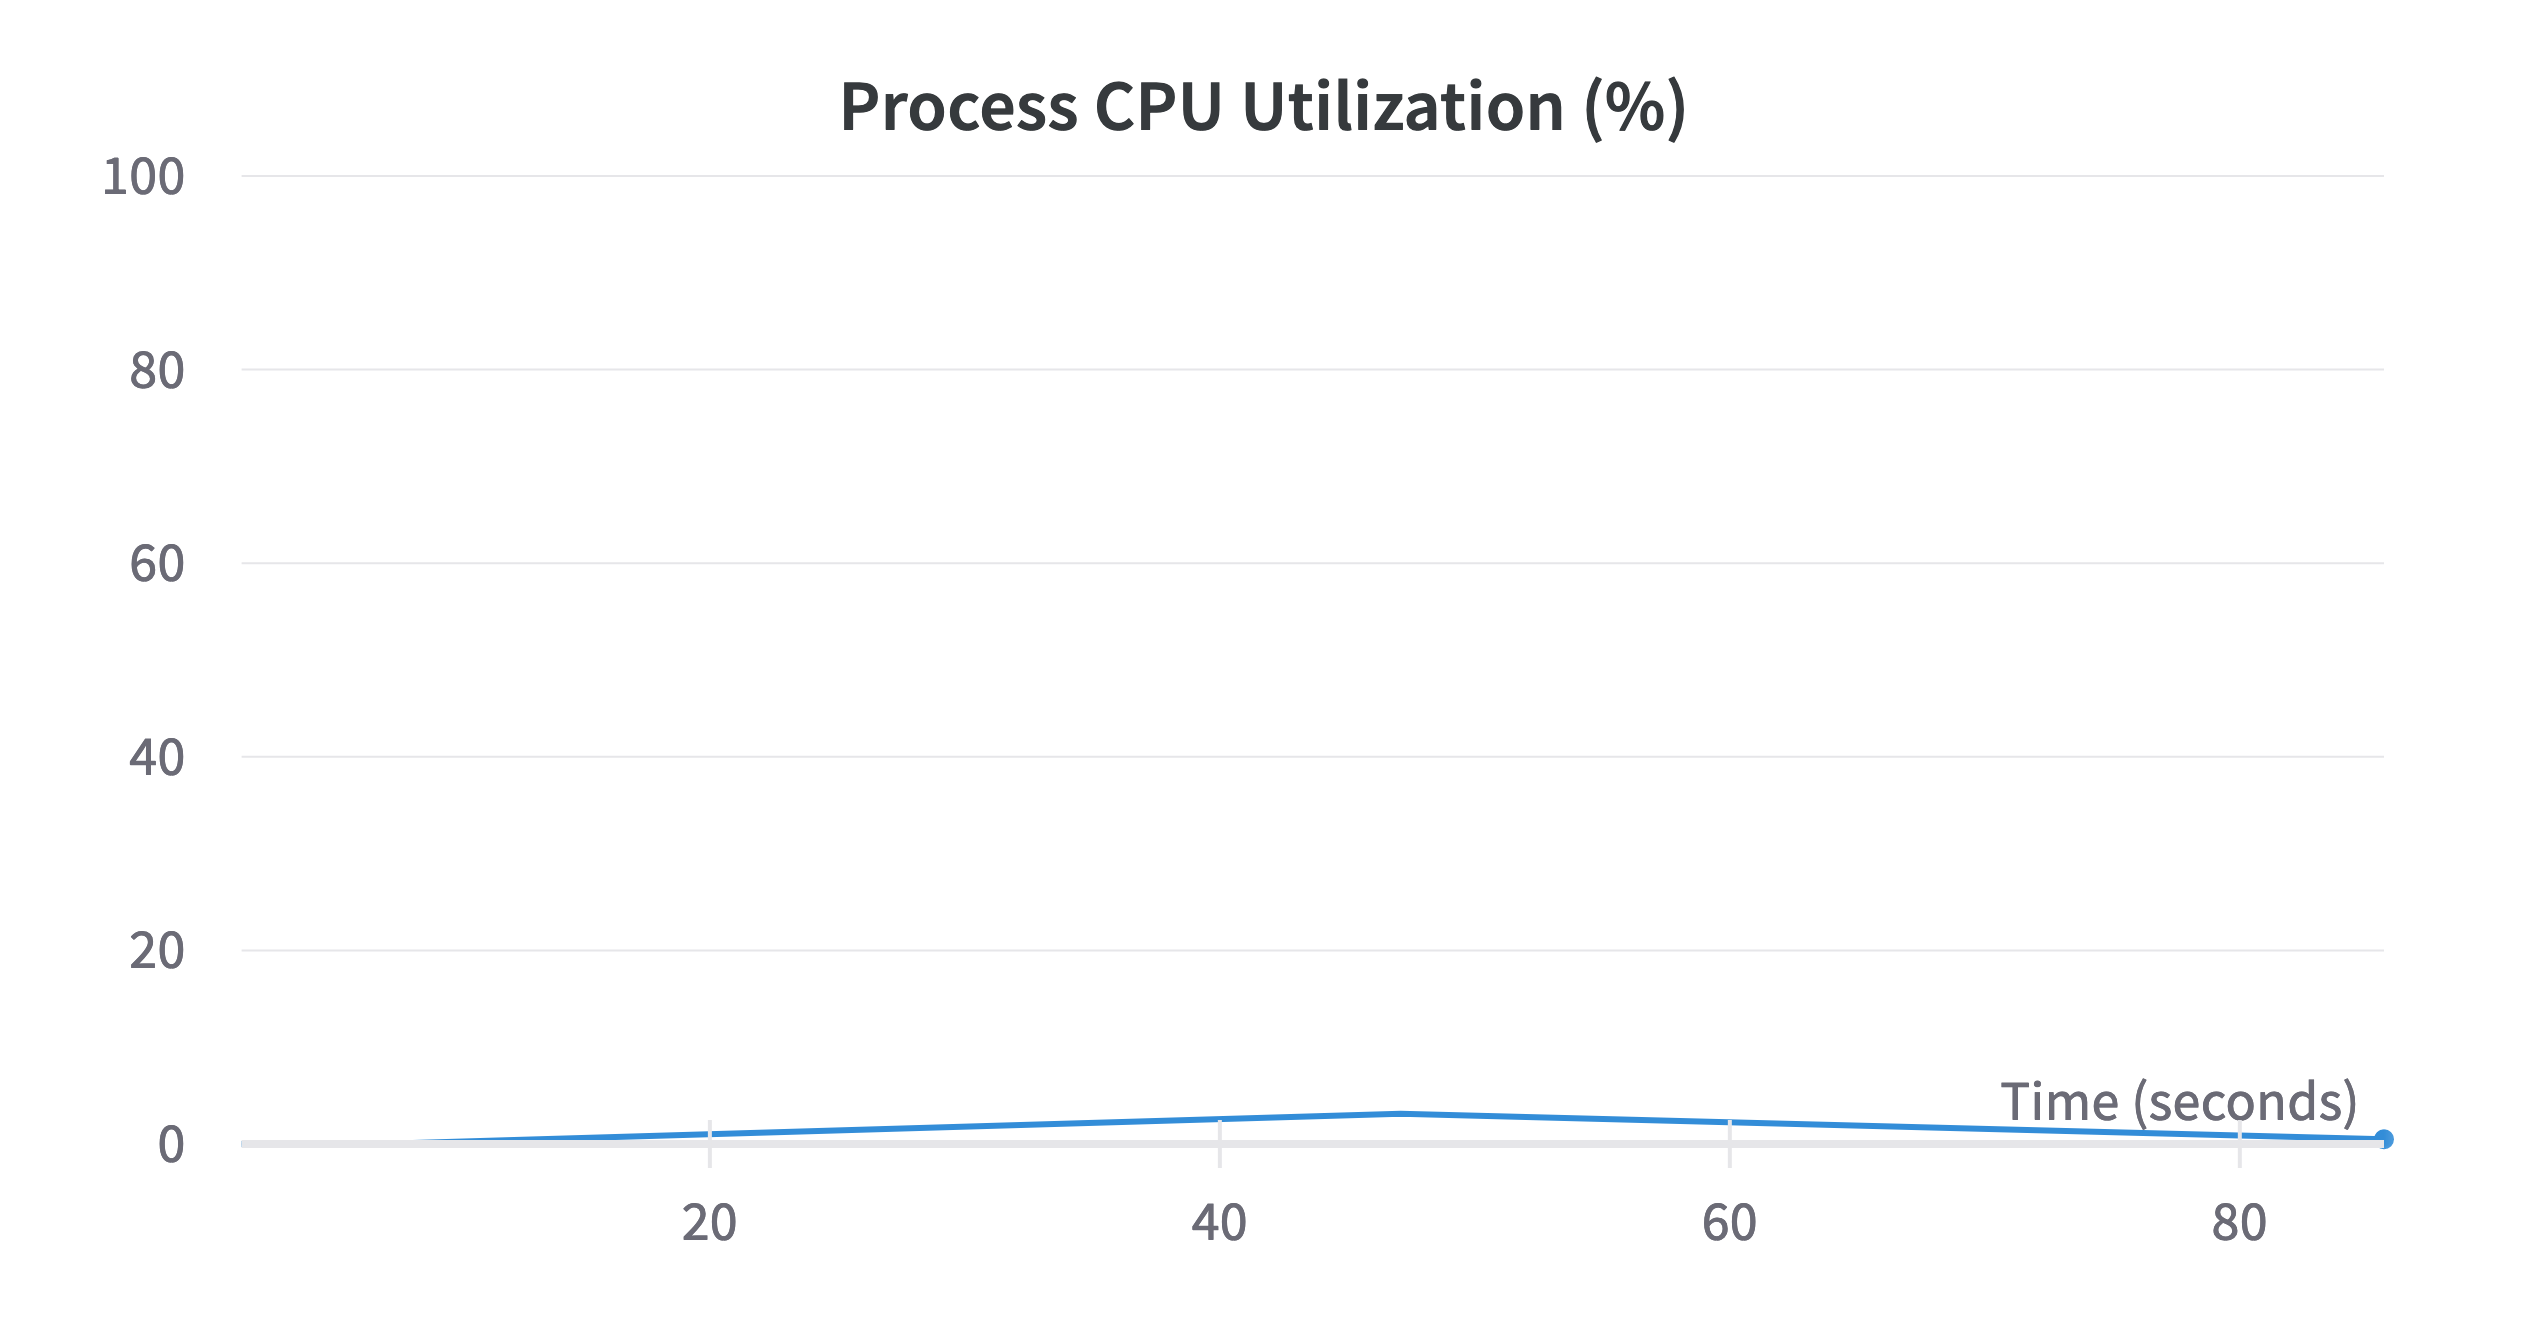
\includegraphics[width=\textwidth]{chapters/3_models/imgs/grrun/grruncputiliziation.png}
	\end{subfigure}
	\begin{subfigure}{0.43\textwidth}
		\centering
		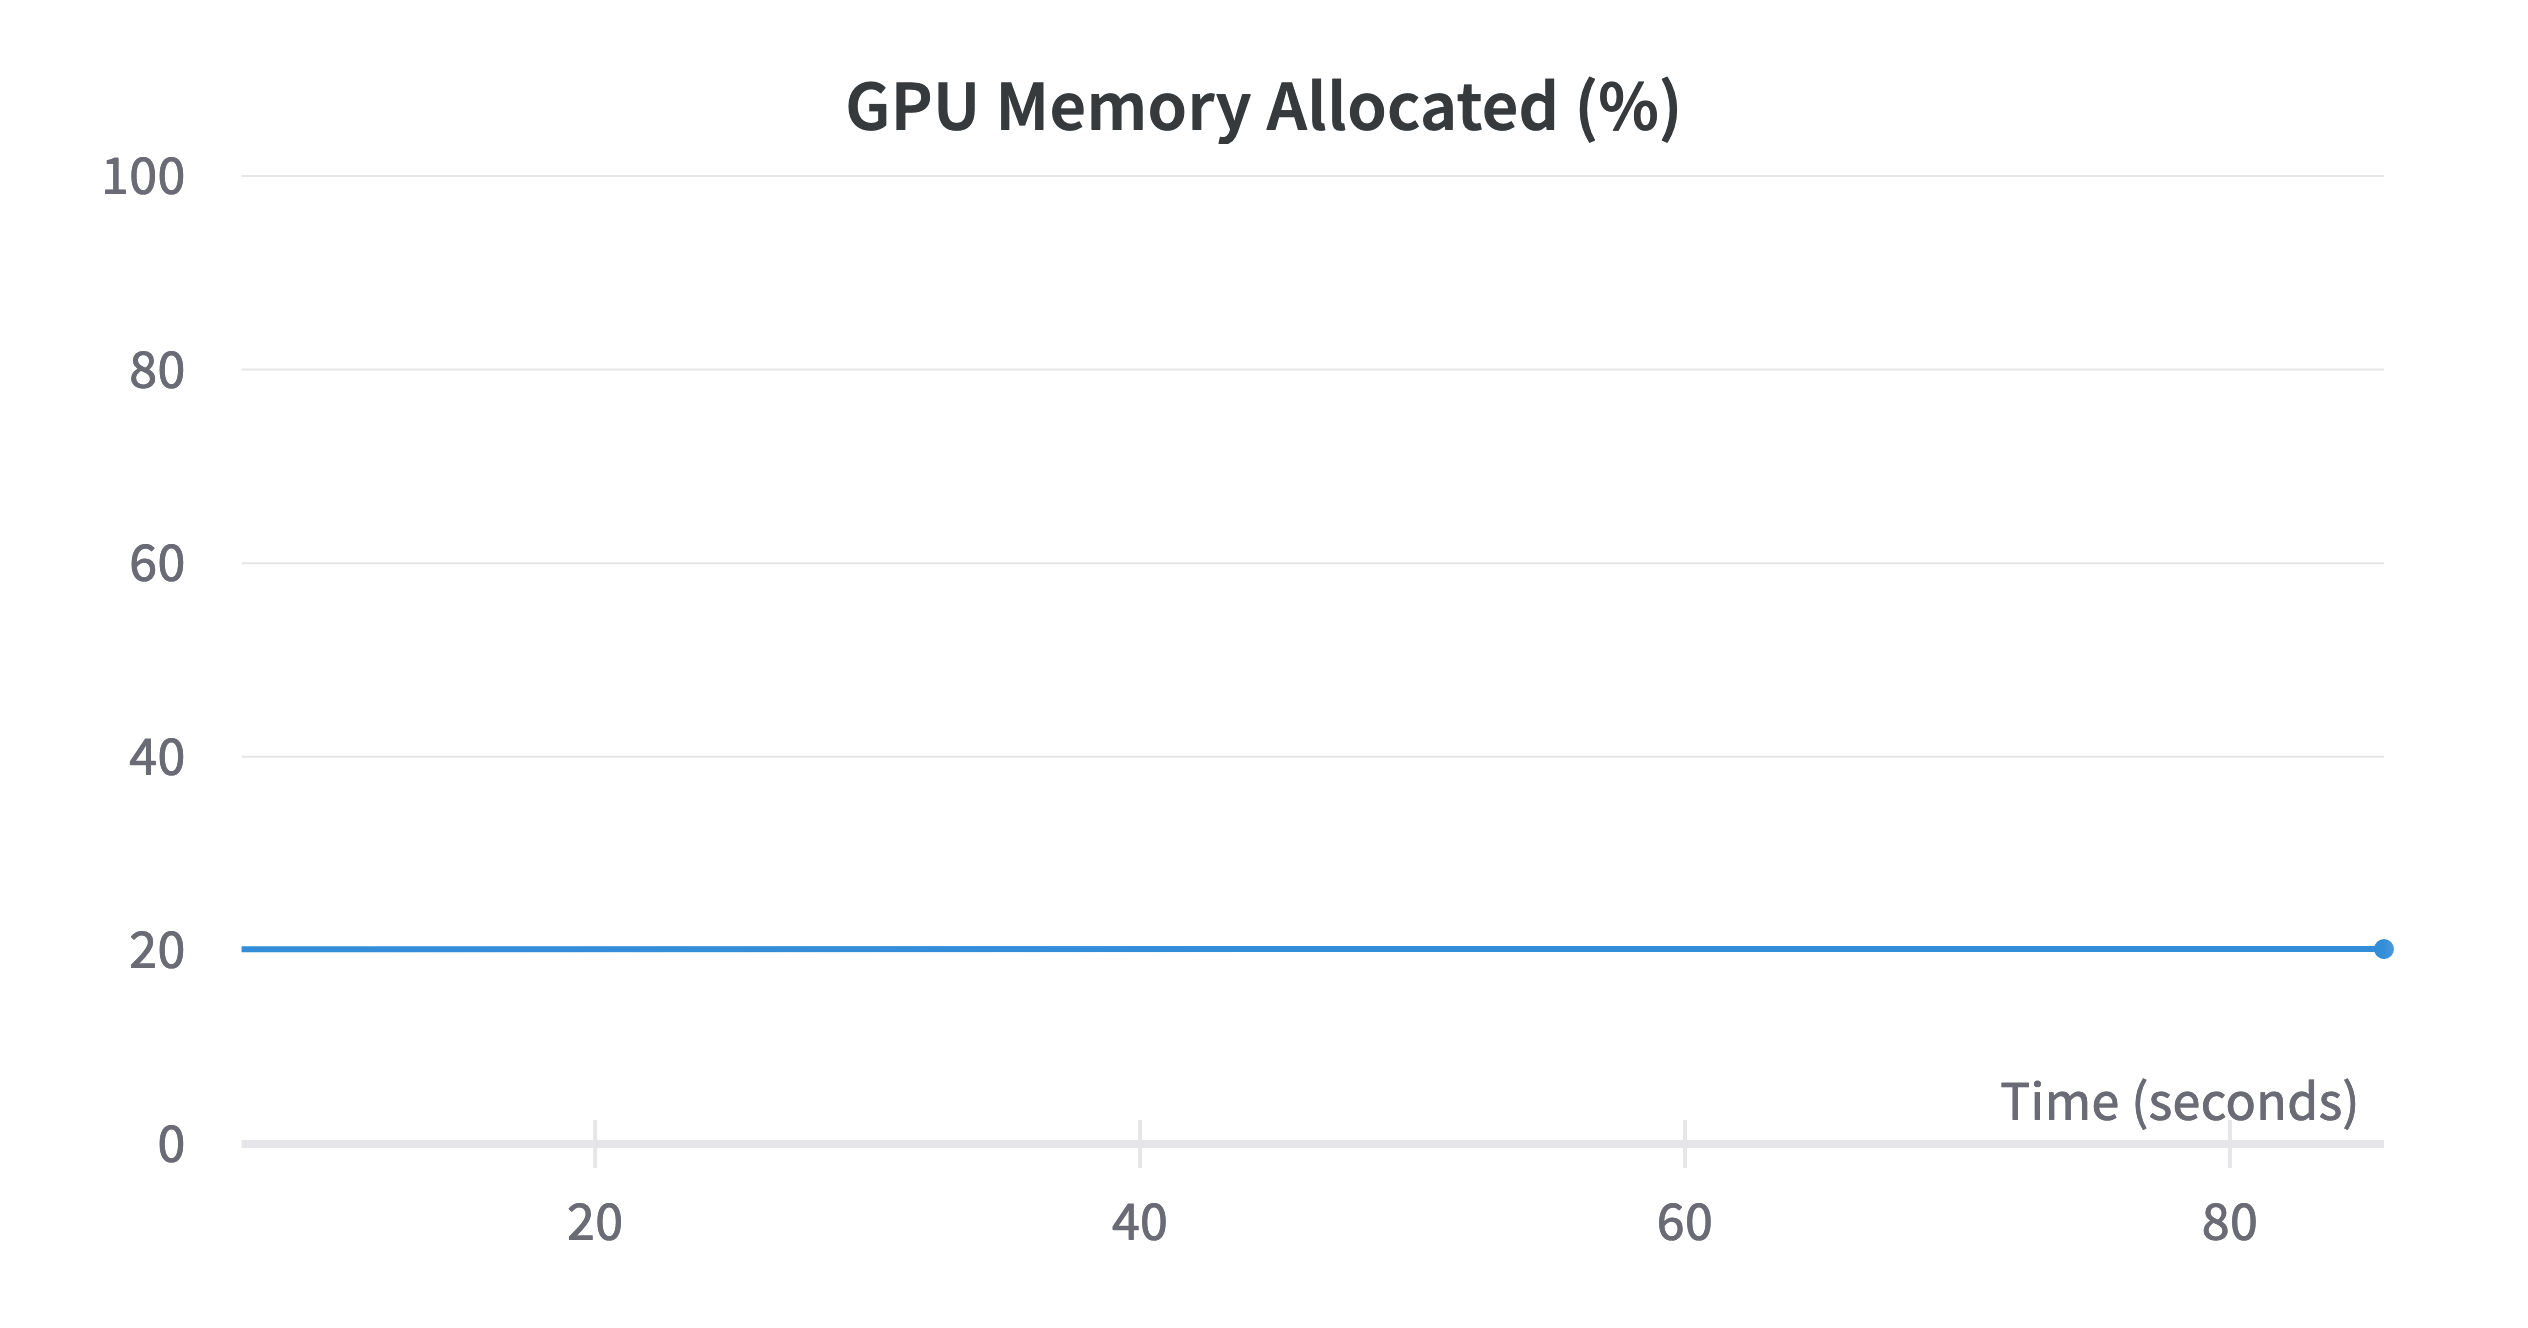
\includegraphics[width=\textwidth]{chapters/3_models/imgs/grrun/grrungpumemalloc.png}
	\end{subfigure}\\
	\begin{subfigure}{0.43\textwidth}
		\centering
		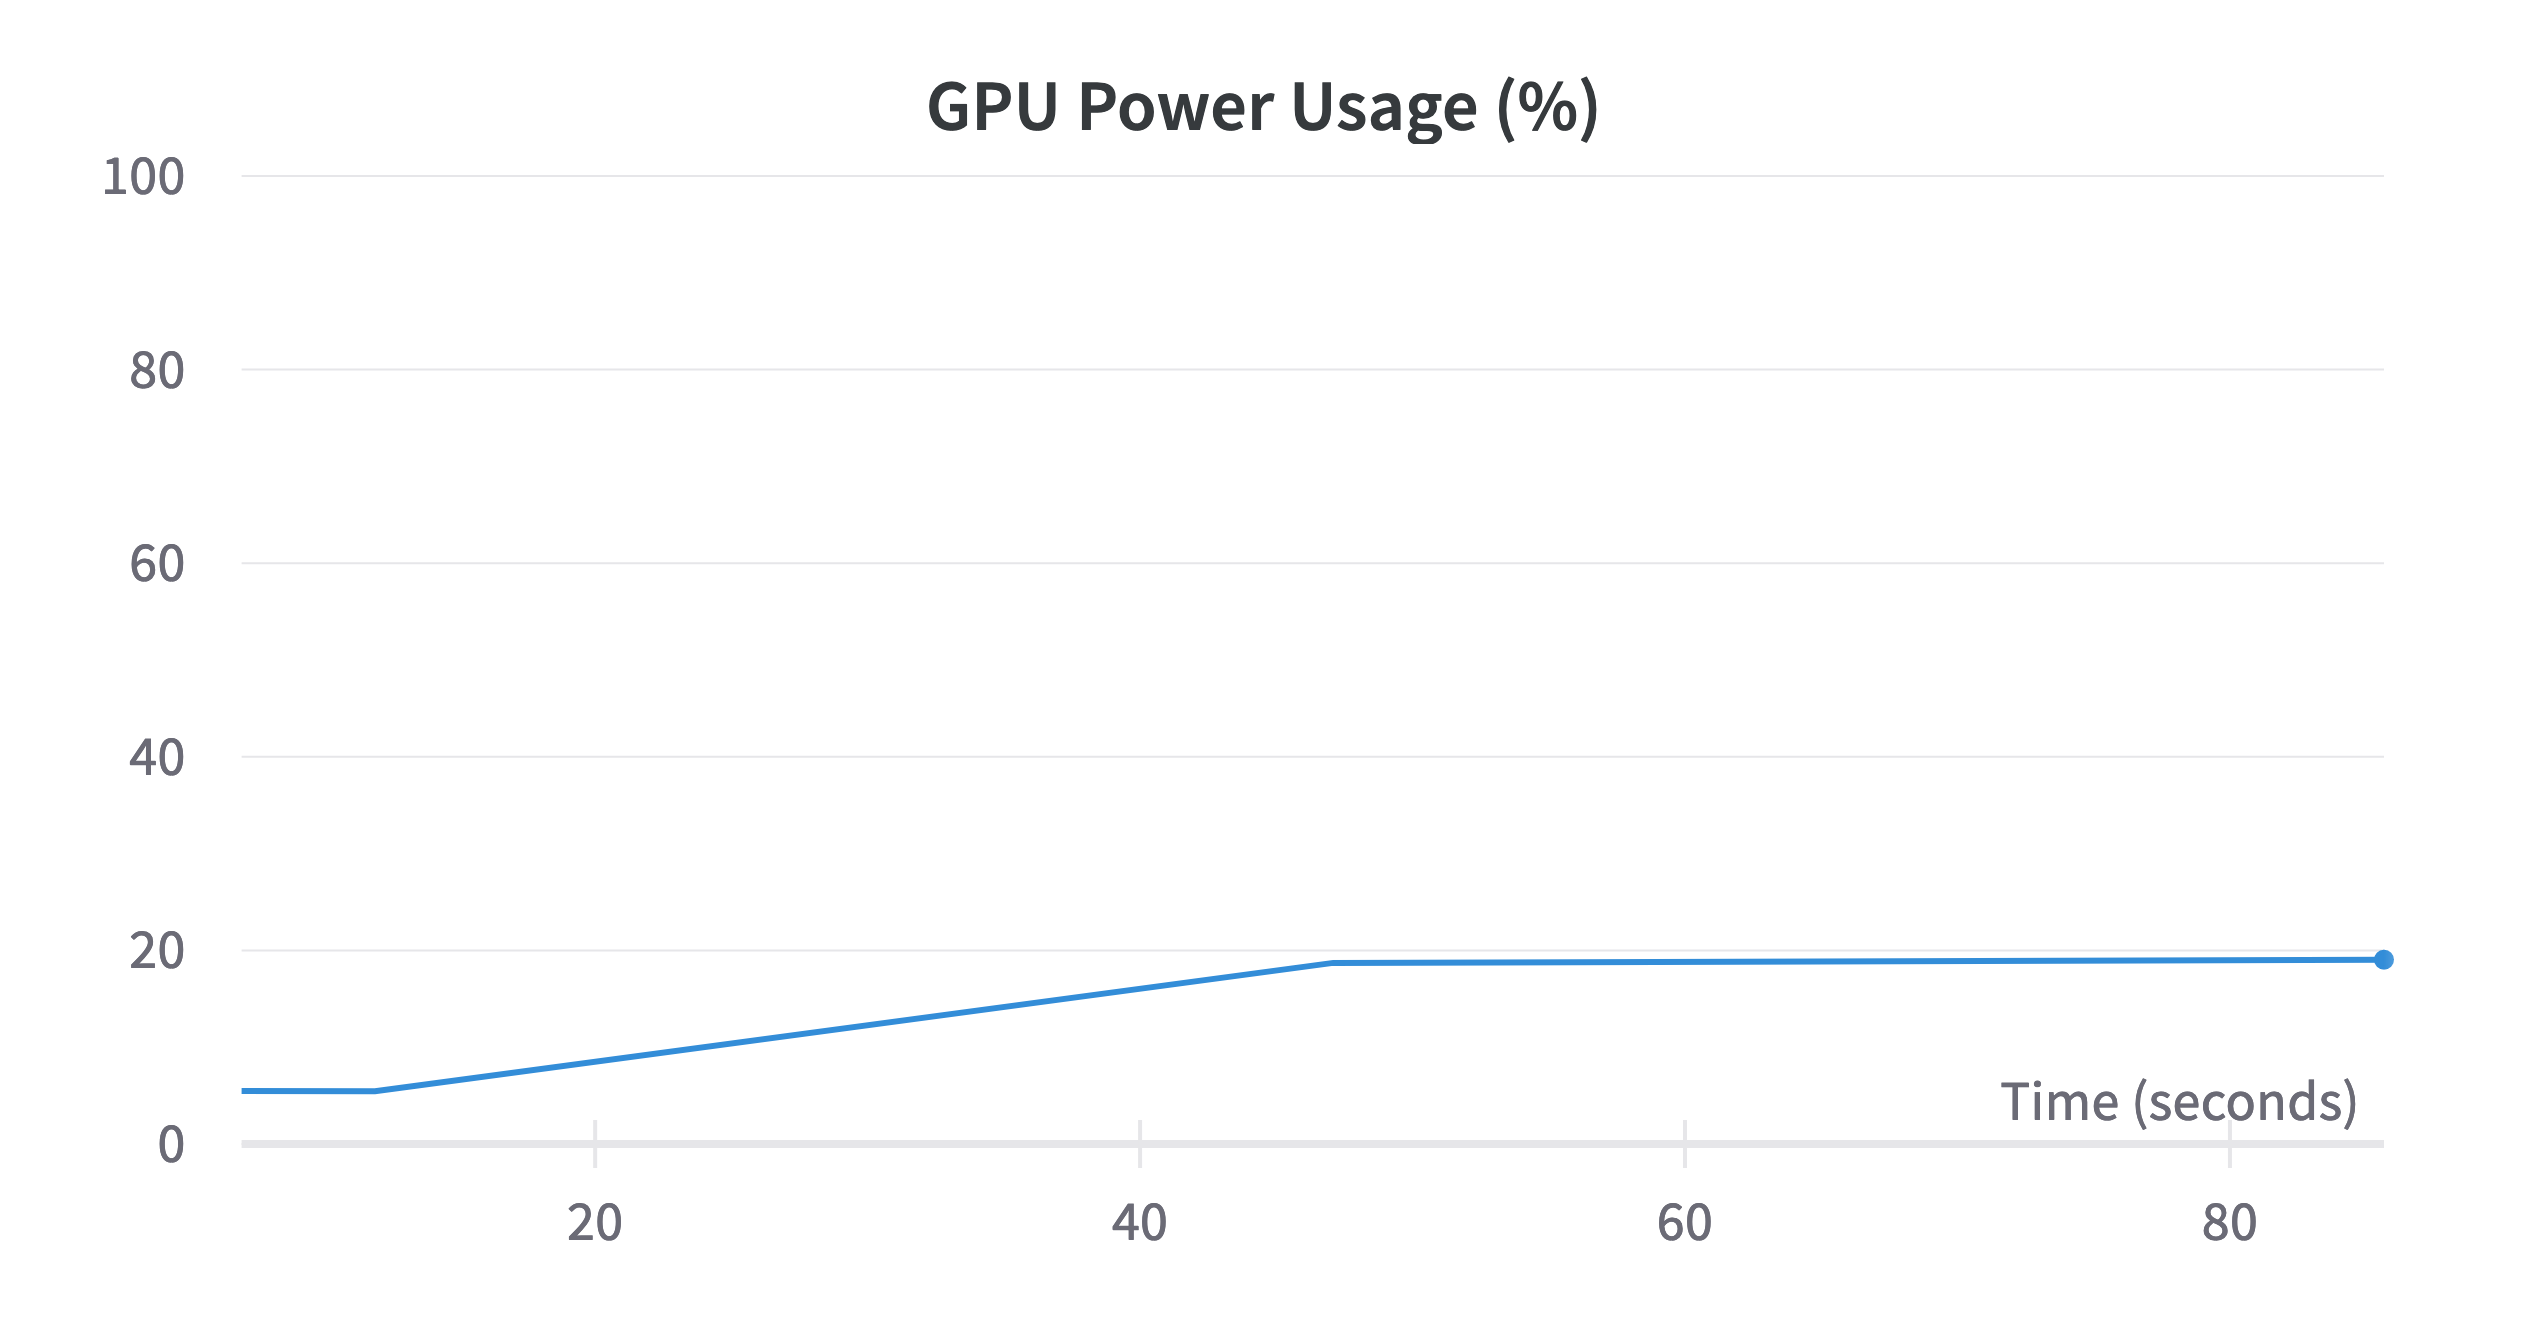
\includegraphics[width=\textwidth]{chapters/3_models/imgs/grrun/grrungpupowerusageperc.png}
	\end{subfigure}
	\begin{subfigure}{0.43\textwidth}
		\centering
		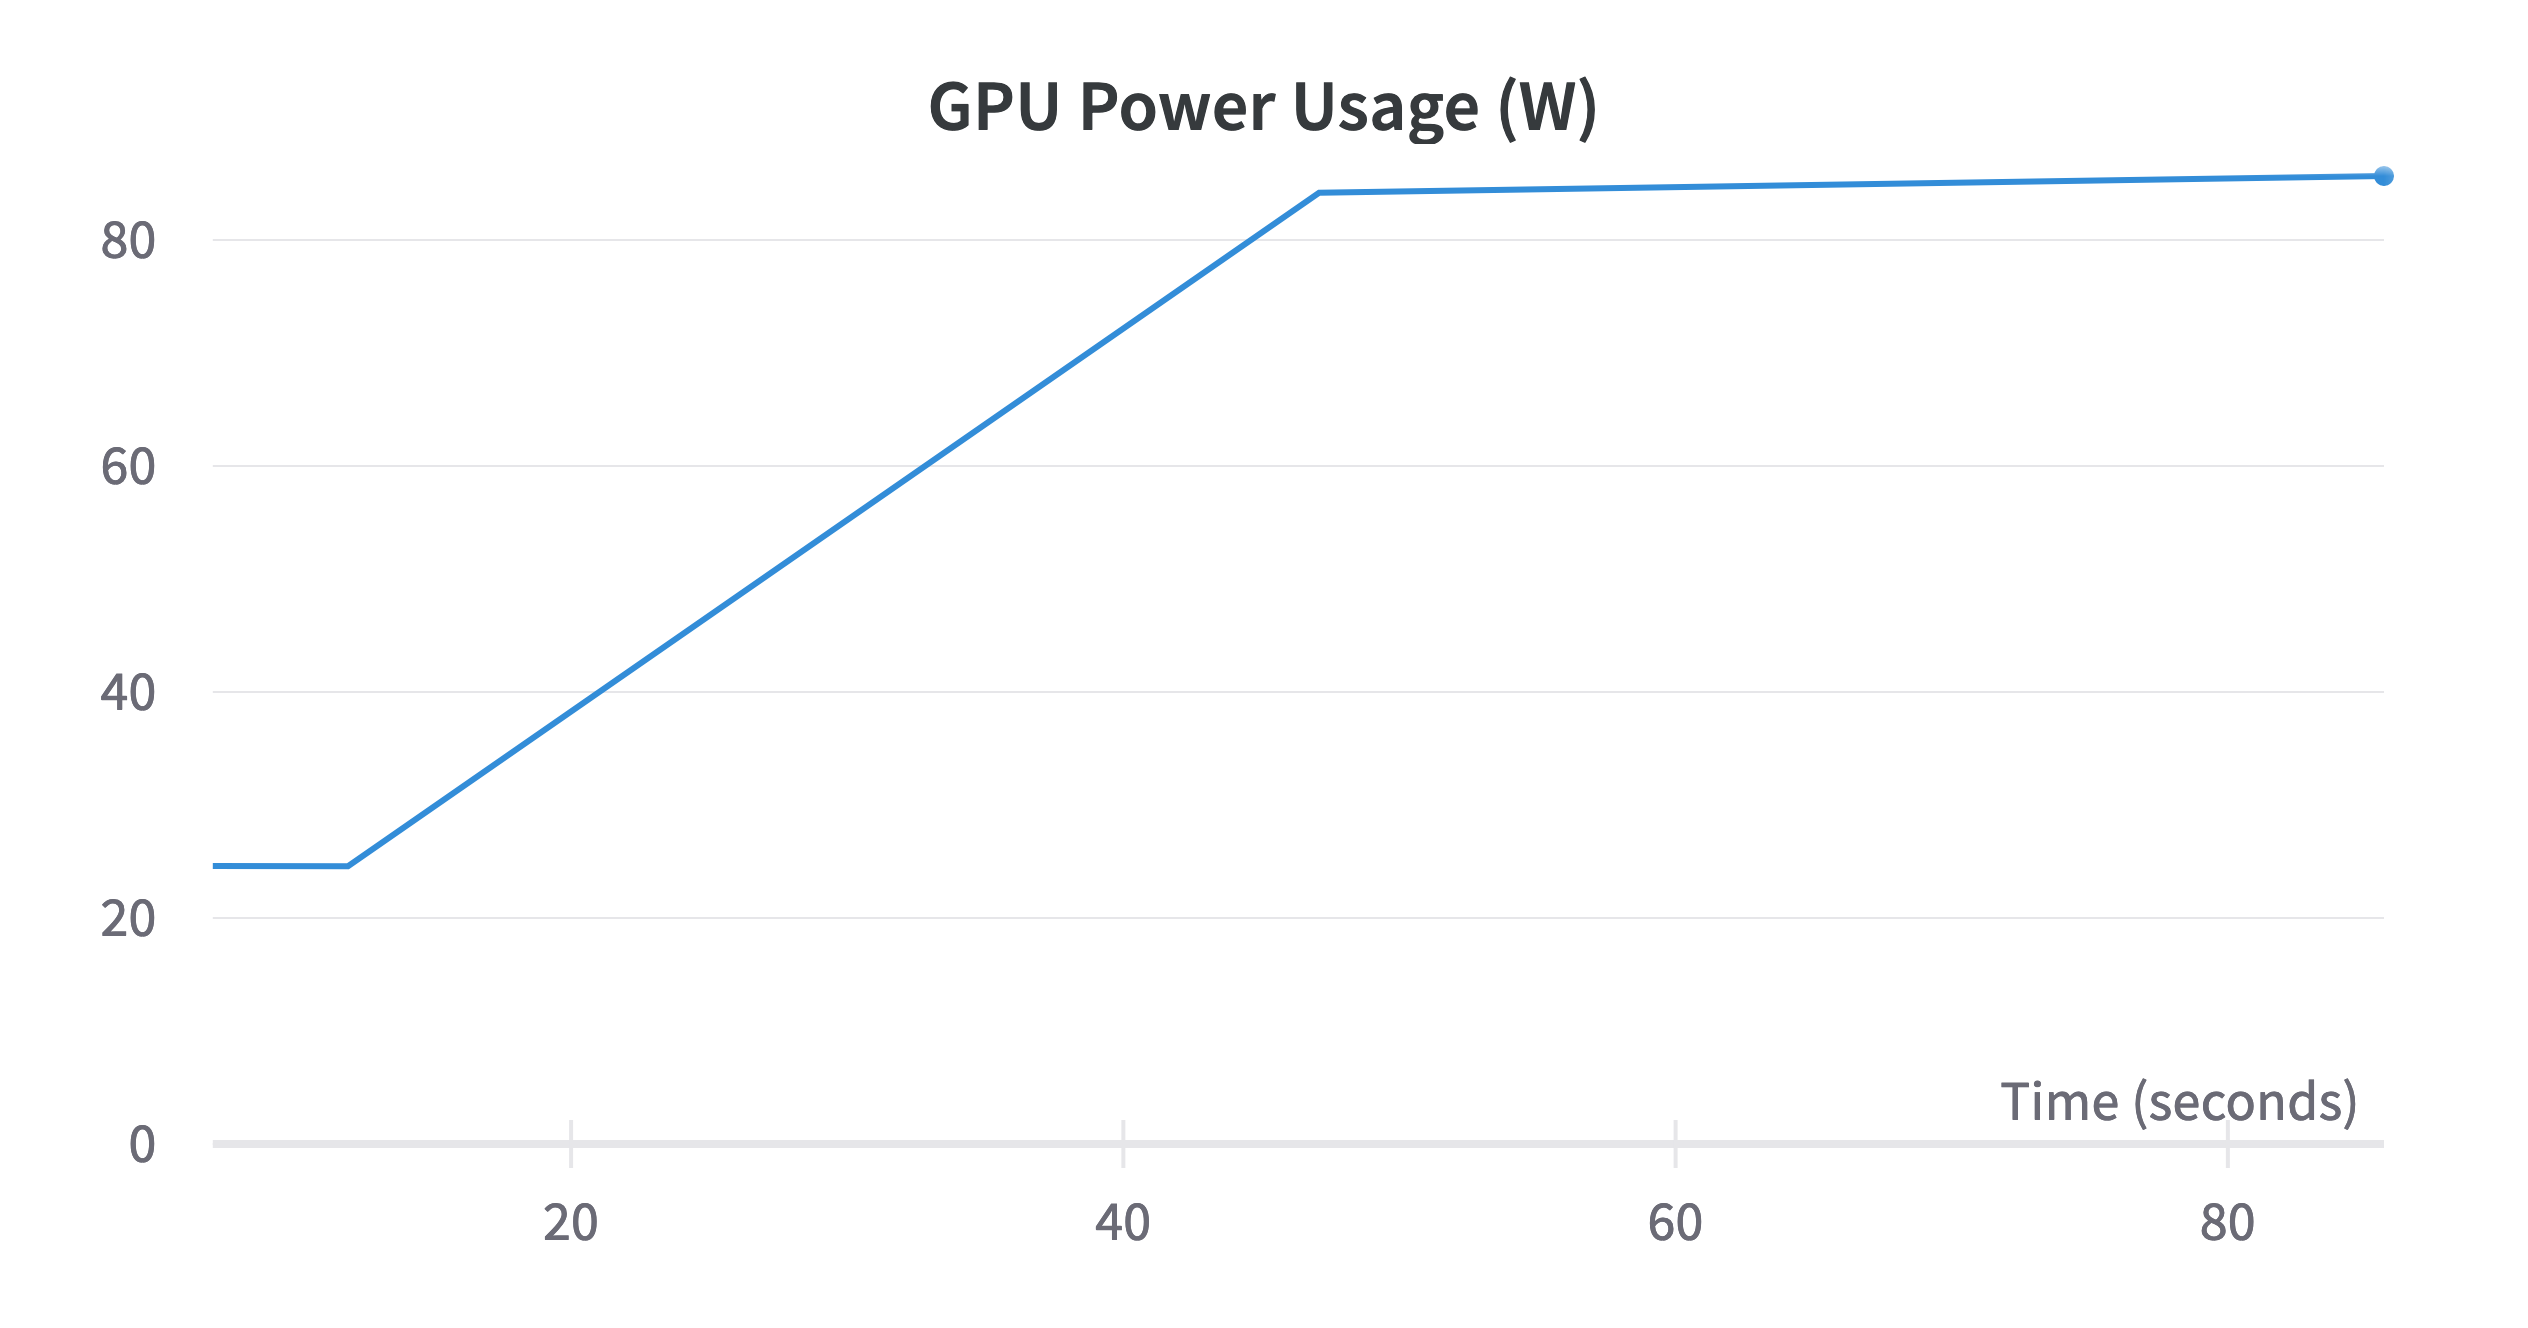
\includegraphics[width=\textwidth]{chapters/3_models/imgs/grrun/grrungpupowerw.png}
	\end{subfigure}\\
	\begin{subfigure}{0.43\textwidth}
		\centering
		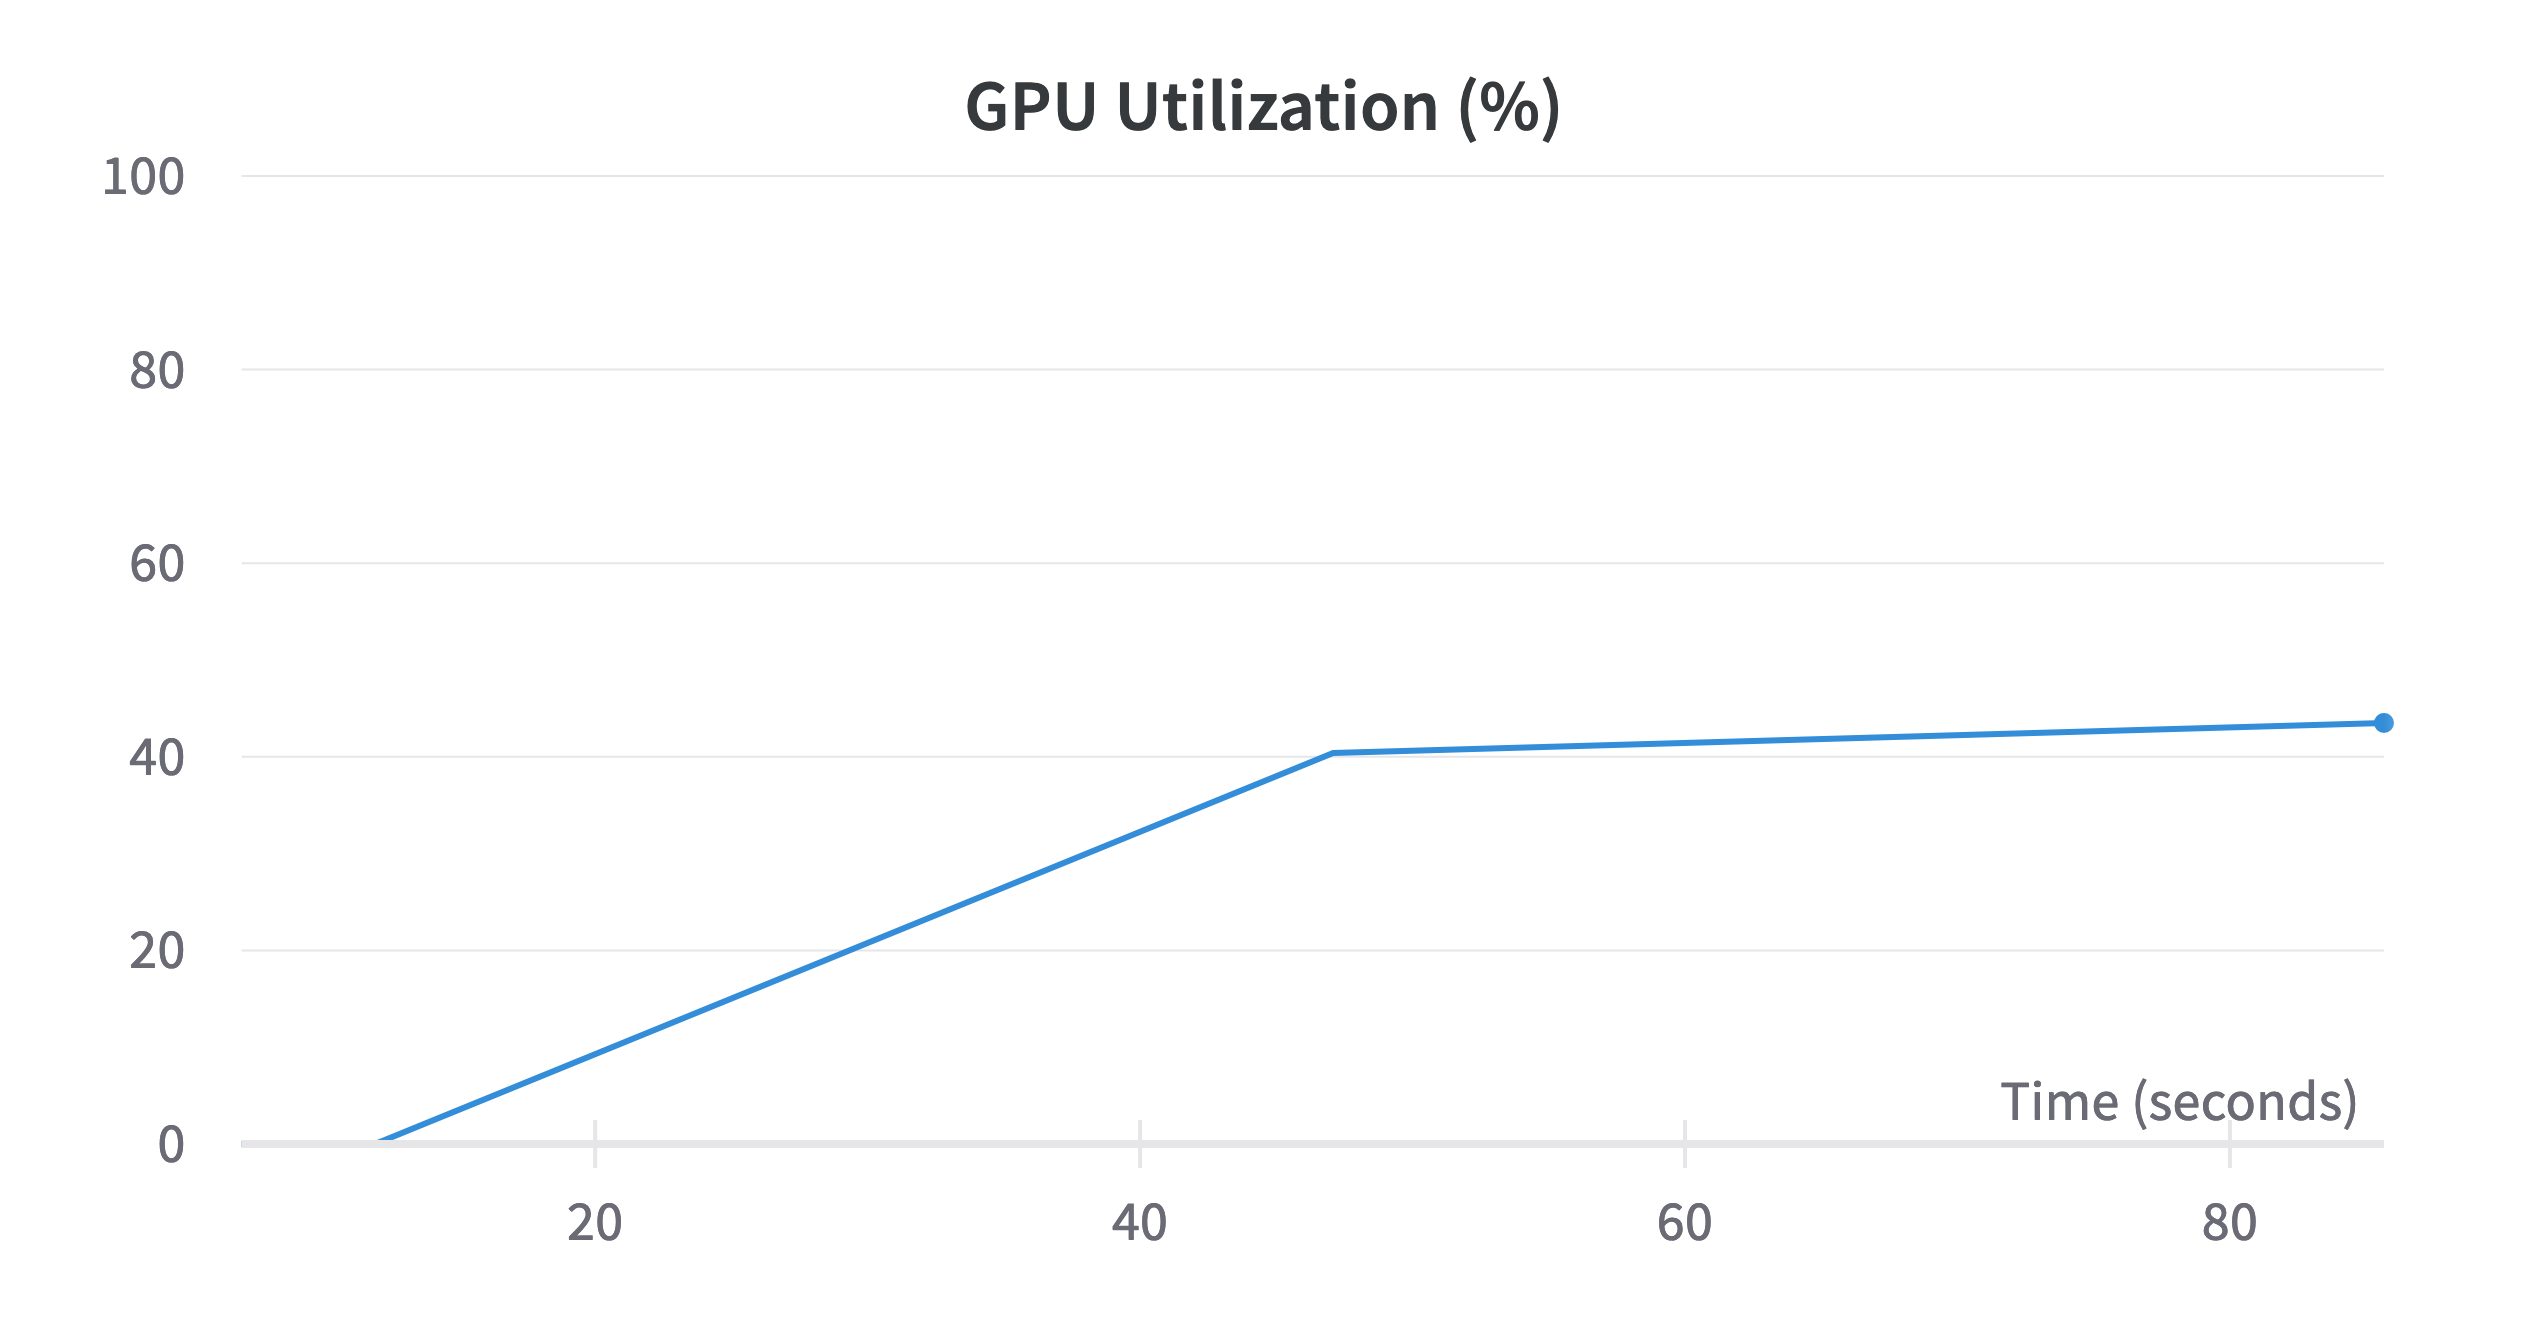
\includegraphics[width=\textwidth]{chapters/3_models/imgs/grrun/grrungputuilizationperc.png}
	\end{subfigure}
	\begin{subfigure}{0.43\textwidth}
		\centering
		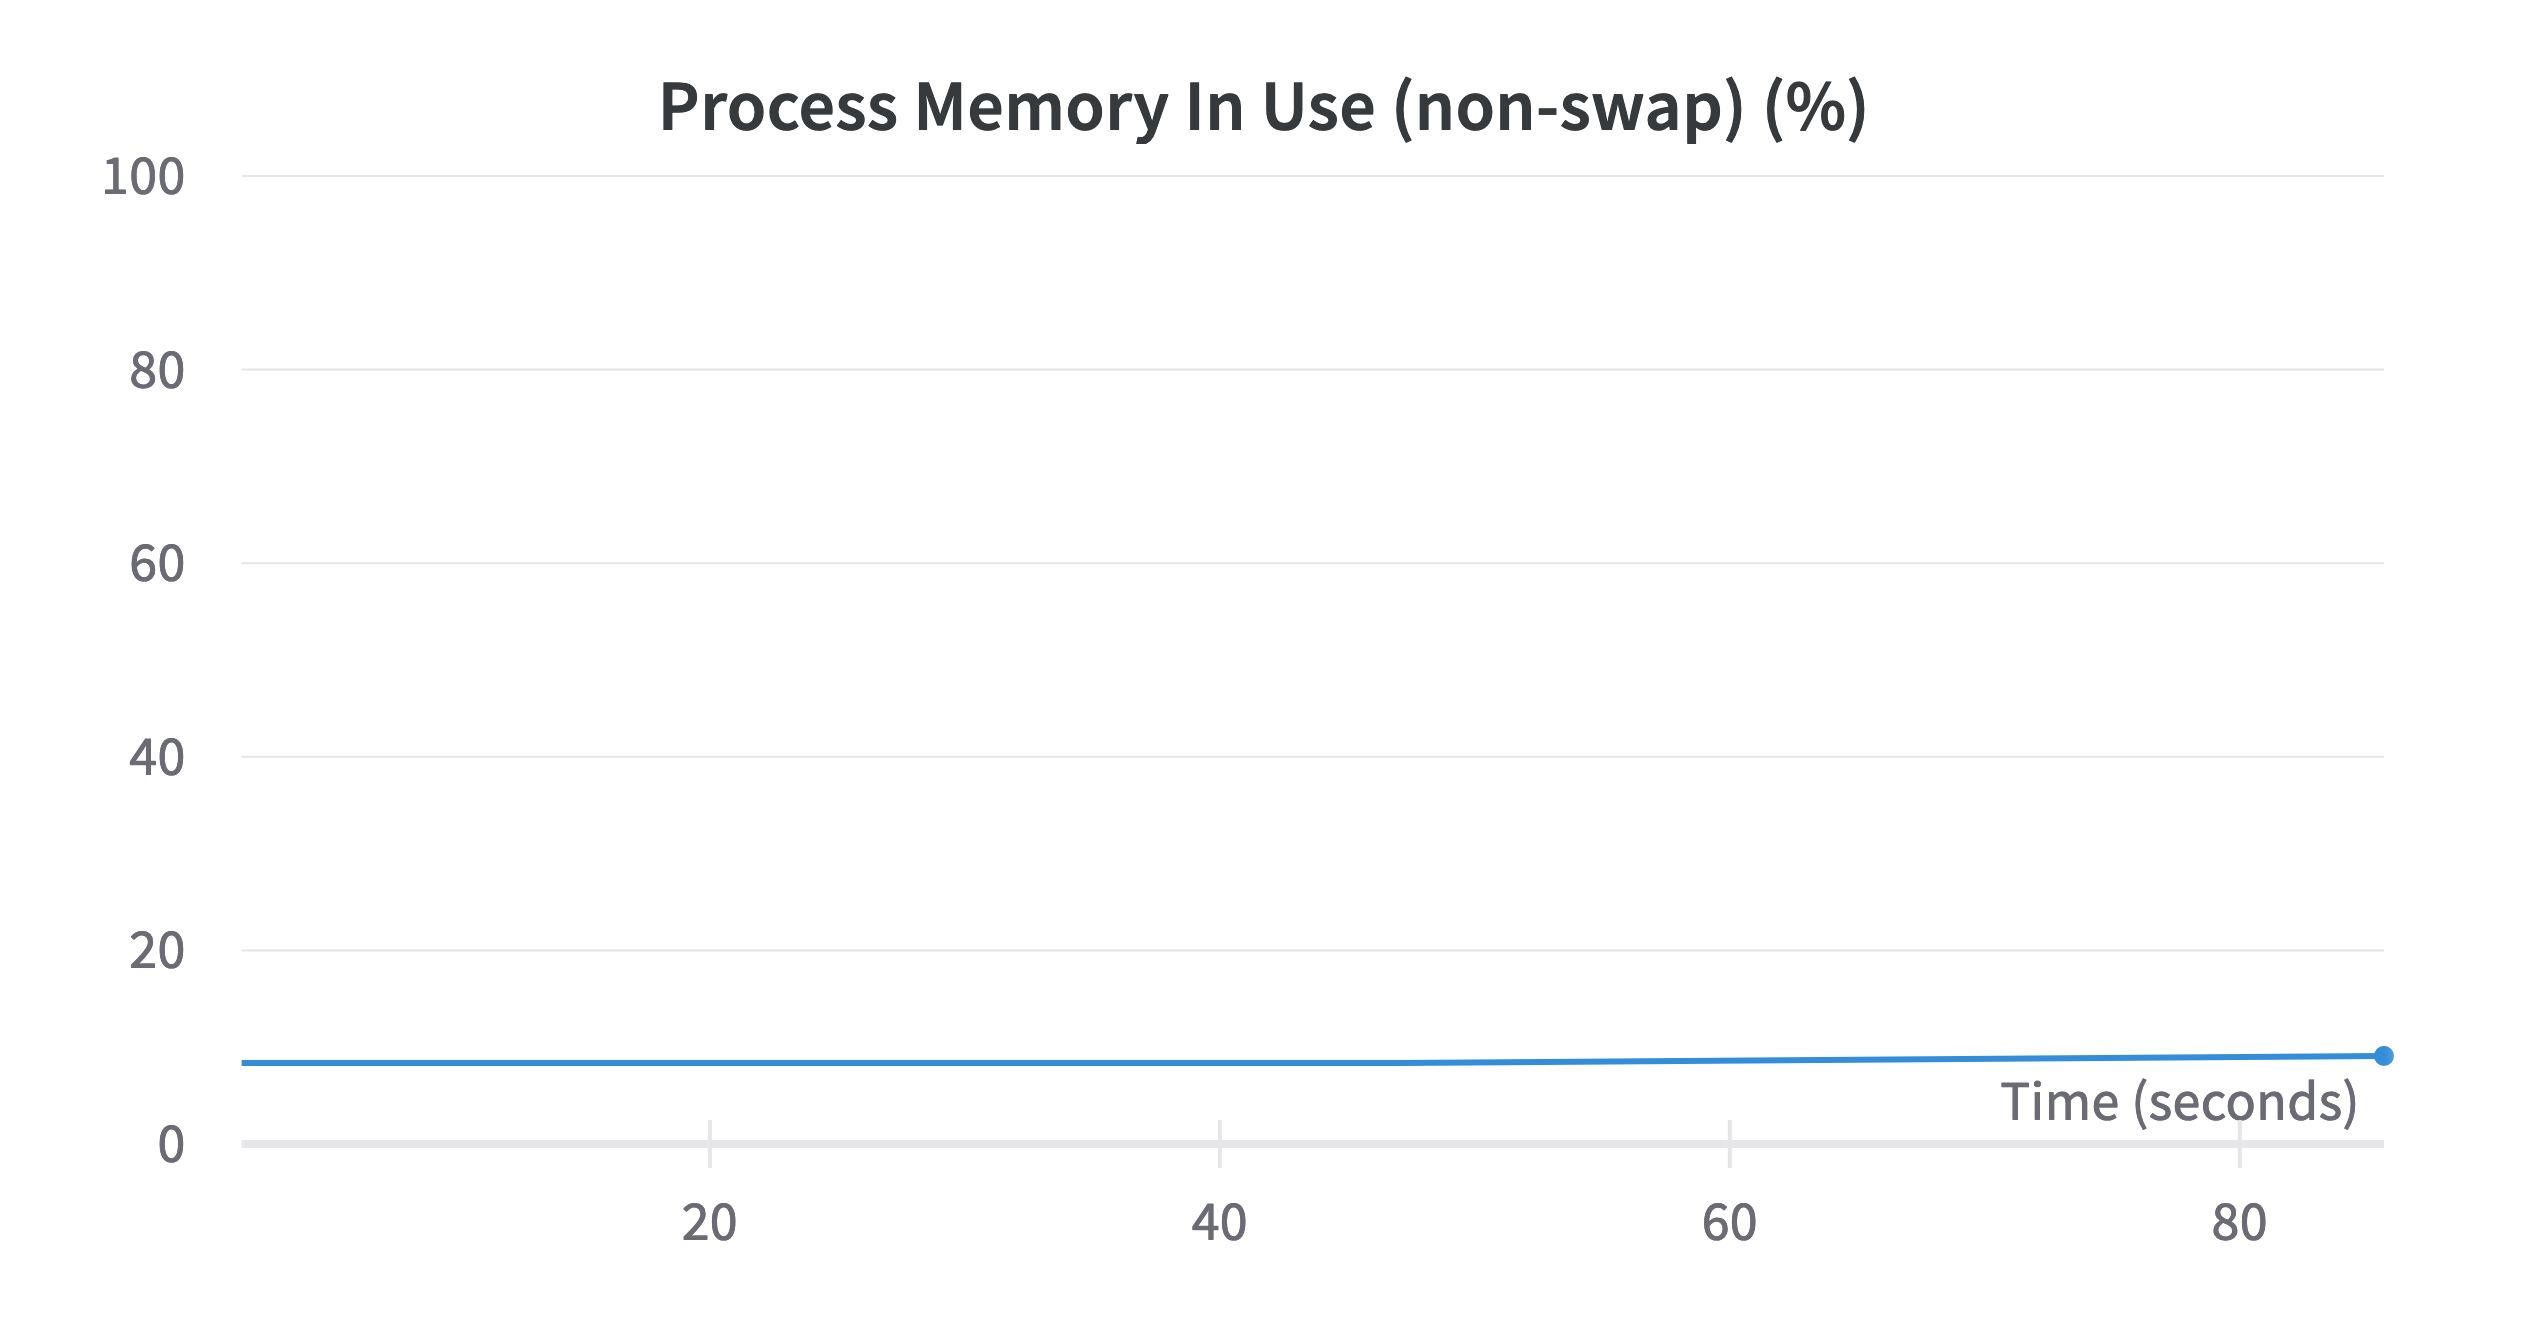
\includegraphics[width=\textwidth]{chapters/3_models/imgs/grrun/grrunmemusage.png}
	\end{subfigure}\\
	\caption{System resources utilized during the Training phase.}
	\label{fig:grrunsysusage}
\end{figure}


\begin{algorithm}[H]
	\caption{RNN model Training Algorithm}\label{alg:grruntraining}
	\begin{algorithmic}
		\Require train/validation datasets; Baseline Neural Network Model

		\State Batch Size $\gets$ 10
		\State Learning Rate $\lambda \gets$ 0.01
		\State Epochs $\gets$ 100
		\State Patience $\gets$ 20
		\State loss $\gets$ L1Loss()
		\State Optimizer $\gets$ Adam Optimizer
		\State Min Gap size $\gets$ 1 day
		\State Max Gap size $\gets$ 4 days
		\State
		\For{\textbf{each} epoch \textbf{in} epochs}
		\For{\textbf{each} (batch\_id, before, after, future, target) \textbf{in} train.next\_batch()}

		\State train\_prediction $\gets$ model(before, after, future) \Comment{Model inference}
		\State train\_prediction $\gets \frac{\text{train\_prediction} \cdot \sum\text{train\_prediction}}{\sum target}$ \Comment{Area normalization}
		\State train\_loss $\gets$ loss(train\_prediction, target)
		\State Optimizer step
		\State Back Propagation
		\EndFor
		\State stop computing gradient
		\For{\textbf{each} (batch\_id, vb, va, vf, vt) \textbf{in} validation.next\_batch()}
		\State val\_prediction $\gets$ model(vb, va, vf) \Comment{Model inference}
		\State val\_prediction $\gets \frac{\text{val\_prediction} \cdot \sum\text{val\_prediction}}{\sum vt}$ \Comment{Area normalization}
		\State val\_loss $\gets$ loss(val\_prediction, vt)
		\EndFor

		\State check for Early Stopping
		\State check for Save Best Result
		\State start computing gradient
		\EndFor
	\end{algorithmic}
\end{algorithm}


\section{Transformers}\label{sec:gab}
Now, we will introduce a third model with an architecture based on Transformers\cite{attention}.
We will analyze its layers, the training phase, highlighting the differences
compared to the previous ones, especially in the construction of the input.
%We will see how this model will prove to be the best among the three models presented in this thesis.

%Ora introdurremo un terzo modello la cui architettura di basa sui 
%Transformers. Andremo ad analizzare la sua architettura, la
%fase di traning evidenziando le differenze rispetto alle precedenti
%soprattutto nella costruzione dell'input e vedremo come questo risulterà 
%essere il migliore tra i tre modelli presentati in questa tesi.

\subsection{Architecture}
The input and operation of this model are slightly different
from what we have seen previously.
This model requires only one tensor as input, representing the data for an entire week, with the \verb|target| feature containing a variable period of values set to \textquote{-1}. This special character, called \textit{placeholder}, indicates to the model the presence of a gap that needs to be filled. %{\bf (*VP* dire meglio che l'input è uno solo invece di più tensori come negli altri modelli, e che il -1 è un placeholder che indica i dati mancanti, se ho capito bene. )}
This gap can have an extremely variable length,
ranging from a minimum of 2 timestamps to the equivalent
of one-third of a week, and it can be positioned anywhere within the week.
This is a very interesting aspect of the model, as it allows it not only to detect the presence of gaps and fill them easily but also enables the immediate construction and preparation of the input.
%Questo è un aspetto molto interessante del modello che gli permette, oltre di poter individuare la presenza dei buchi e di chiuderli in modo semplice, permette anche una costruzione e preparazione immediata dell'input.
%{\bf (*VP* aggiungi una frasetta per dire che questa è una caratteristica interessante del modello che ne permette una applicabilità più ampia, più generale. Sempre se ho capito bene.)}

The model's objective is to learn to predict the entire week, including the gap.
Through a masking system, we can then extract only the values of interest.
Let's now delve into the specific elements that characterize and make up this model:


%L'input ed il funzionamento di questo modello è leggermente differente
%da quelli che abbiamo visto in precedenza. Questo necessita di
%un'intera settimana in input con al suo interno un buco che viene
%rappresentato da una sequenza di caratteri speciali, nello specifico \textquote{-1}. Questo buco potrà avere una lunghezza estremamente variabile:
%da un minimo di 2 timestamp fino all'equivalente di un terzo di settimana
%e potrà essere posizionato ovunque all'interno di questa.
%Il modello avrà quindi l'obbiettivo di apprendere a predirre 
%tutta la settimana, compreso il buco, e tramite un sistema di maschere
%saremmo in grado poi di poter estrapolare solo i valori di nostro
%interesse.
%
%Analizziamo ora nel dettaglio i principali elementi che caratterizzano e compongono questo modello:

\begin{itemize}
	\item \textbf{Input}: As described earlier,
	      the input is a tensor containing one week of data with the
	      target feature that includes a period of -1 (representing the gap).
	\item \textbf{Convolution}: The input goes through two convolutional layers to extract and understand the most important and representative features of the time series. Each layer undergoes batch normalization, and the Gaussian Error Linear Units (GELU)\cite{gelu} function is used as the activation function.
	\item \textbf{Positional Encoder}: To help the model understand the temporal sequence and the order of the different time series, a positional encoder called Time Absolute Position Encoding (tAPE)\cite{tape} is implemented. It incorporates the series length and input embedding dimension for absolute position encoding\cite{tape}.
	\item \textbf{Transformer Encoder}: After performing positional encoding on the output of the convolutional layers, it is passed to the transformer. This transformer\cite{attention} consists of 2 transformer layers, each of which contains 8 heads for multi-head attention\cite{attention}, 64 layers for the feed-forward part, a dropout rate of 0.1, and GELU as the activation function.
	\item \textbf{Output}: This is the final layer of the network, responsible for reshaping the transformer's output to the required dimension for use. It is a feed-forward layer with an output dimension of 1, and it applies the Softplus\cite{functions} function as the activation function.
\end{itemize}

%\begin{itemize}
%    \item \textbf{Input}: come descritto prima, un tensore contenente
%    sempre 1 settimana di dati con all'interno la feature target che presenta un periodo con valori di -1 (buco).
%    \item \textbf{Convoluzione}: l'input viene passatro attraverso
%    due livelli Convolutivi per cercare di ottenere e comprendere
%    le feature più importanti e rappresentative della serie.
%    Ad ognuno di questi viene applicata una procedura di Batch
%    Normaization ed impiegata la Gaussian Error Linear Units (GELU) come funzione di attivazione.
%    \item \textbf{Positional Encoder}: per peremttere al modello
%    di comprendere la successione del tempo e l'ordinamento
%    delle varie serie temporali abbiamo implementato il positional encoder time Absolute Position Encoding (tAPE), il quale incorporates 
%    the series length and input embedding dimension in absolute
%    position encoding.
%    \item \textbf{Transformer Encoder}: una volta effettuato il positional
%    encoding dell'output dei layer convolutivi, questo viene passato
%    al transformer. Questo è formato da 2 Transformers Layer ed ognuno
%    di questi è composto da 8 heads per la multiheadattention, 64 layer per la parte Feed Forward, 0.1 come valore
%    di dropout e la GELU come activation function.
%    \item \textbf{Output}: è l'ultimo livello della rete e si occupa di
%    riportare la dimensione dell'output del Transformer a quella necessaria
%    per poter essere utilizzata. \'{E} un layer feed forward con la dimensione dell'output pari a 1 e viene applicata la Softplus come
%    funzione di attivazione.
%\end{itemize}

\begin{figure}[H]
	\centering
	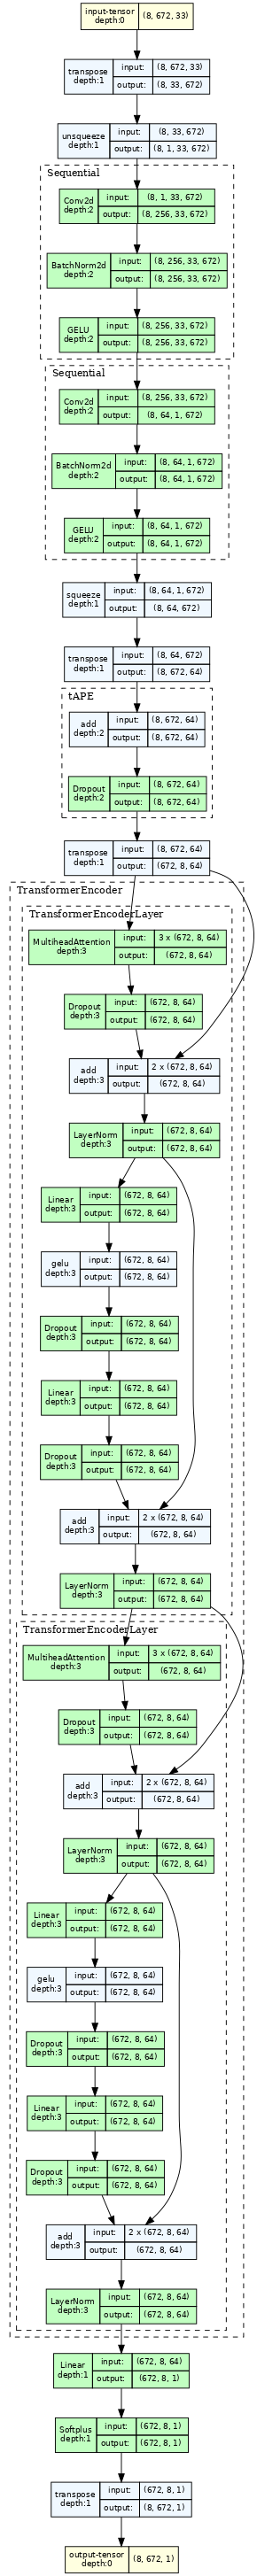
\includegraphics[height=\textheight]{chapters/3_models/imgs/gab/transformerarchitecture.png}
	\caption{Transformer Based Model architecture visualization.}\label{fig:gabarchitecture}
\end{figure}

\subsection{Training}
The model was trained using the input format discussed earlier,
generating gaps artificially in the training dataset, while also ensuring the
creation of a gap mask.
This mask is an array of the same length as the input time series,
composed of two elements: 1 to indicate the gap timestamps and 0 for regular timestamps.
This allows obtaining only the predicted values within the gap,
which are used for evaluating the loss function.

In this case, a procedure for normalizing the area was applied to ensure that the
model learns the gap curve's behavior.
The L1Loss (Equation~\ref{eq:l1loss}) function was employed as the loss function, and AdamW\cite{adamw} was used as the
optimizer with a learning rate ($\lambda$) set to 0.00001.
The learning rate is then adjusted during training using a cosine annealing scheduler\cite{scheduler1}\cite{scheduler2}
to provide optimal conditions for the model during this phase.

Additionally, a validation dataset was used to assess the model's
performance during training and to enable the
\textit{Early Stopping} and \textit{Save Best} procedures,
which were also used in this case.

	{\bf (*VP* valgono anche qui tutte le cose dette prima. Sarebbe opportuno giustificare la forma dei grafici reltaivi all'uso dlle risorse, visto che hanno una forma diversa (a trapezio) rispetto a quelle precedenti. Ovviamente se sai giustificarlo, altrimenti lascia stare.)}

%Il modello è stato allenato utilizzando il formato di input discusso in
%precedenza andando a creare buchi in modo artificiale nel dataset
%di training facendo attenzione a generare anche una maschera del buco: un
%array di lunghezza pari a quella della serie passata in input e coposto da due elementi, 1 indica i timestamp del buco mentre 0 quelli ordinari.
%In questo modo sarà possibile andare ad ottenere solo i valori del buco
%predetti dal modello per poi valutare la loss function solo su questi valori.
%Anche in questo caso è stata applicata una procedura di normalizzazione dell'area
%per assicurarci che il modello impari ad apprendere l'andamendo della curva
%del buco. E' stata impiegata la L1Loss come loss function, AdamW come
%optimizer con learning rate $\lambda$ pari a 0.00001 che poi 
%verrà variato durante la procedura di training tramite un cosine annealing scheduler per permettere al modello le migliori condizioni durante questa
%fase.
%Anche in questo caso è stato impiegato il dataset di validation per andare
%a misurare le performance del modello durante l'allenamento e per permettere
%il funzionamento delle procedure 
%\textit{Early Stopping} e \textit{Save Bast} che anche inquesto caso 
%sono state implementate.

\begin{table}[H]
	\begin{center}
		\begin{tabular}[c]{l|l}
			\textbf{Total Parameters (\#)}     & 594177 \\
			\textbf{Trainable Parameters (\#)} & 594177 \\
			\textbf{Training Duration (s)}     & 900.0  \\
			\textbf{Model Size (MB)}           & 2.4
		\end{tabular}
	\end{center}
	\caption{Transformer based model specification.}\label{tab:gabspecs}
\end{table}

\begin{figure}[H]
	\centering
	\begin{tikzpicture}
		\draw[->] (-3,0) -- (3,0) node[right] {$x$};
		\draw[->] (0,-1) -- (0,2) node[above] {$y$};
		\draw[dotted] (-3,-1) grid (3,2);
		\draw[color=blue, domain=-3:2] plot[id=logistic] function{0.5 * x * (1+tanh(sqrt(2/pi) * (x + 0.044715*x**3)))};
	\end{tikzpicture}
	\caption{Gaussian Error Linear Units (GELU). $GELU(x) = x * \Phi(x)$}
	\label{fig:gelu}
\end{figure}

\begin{figure}[H]
	\centering
	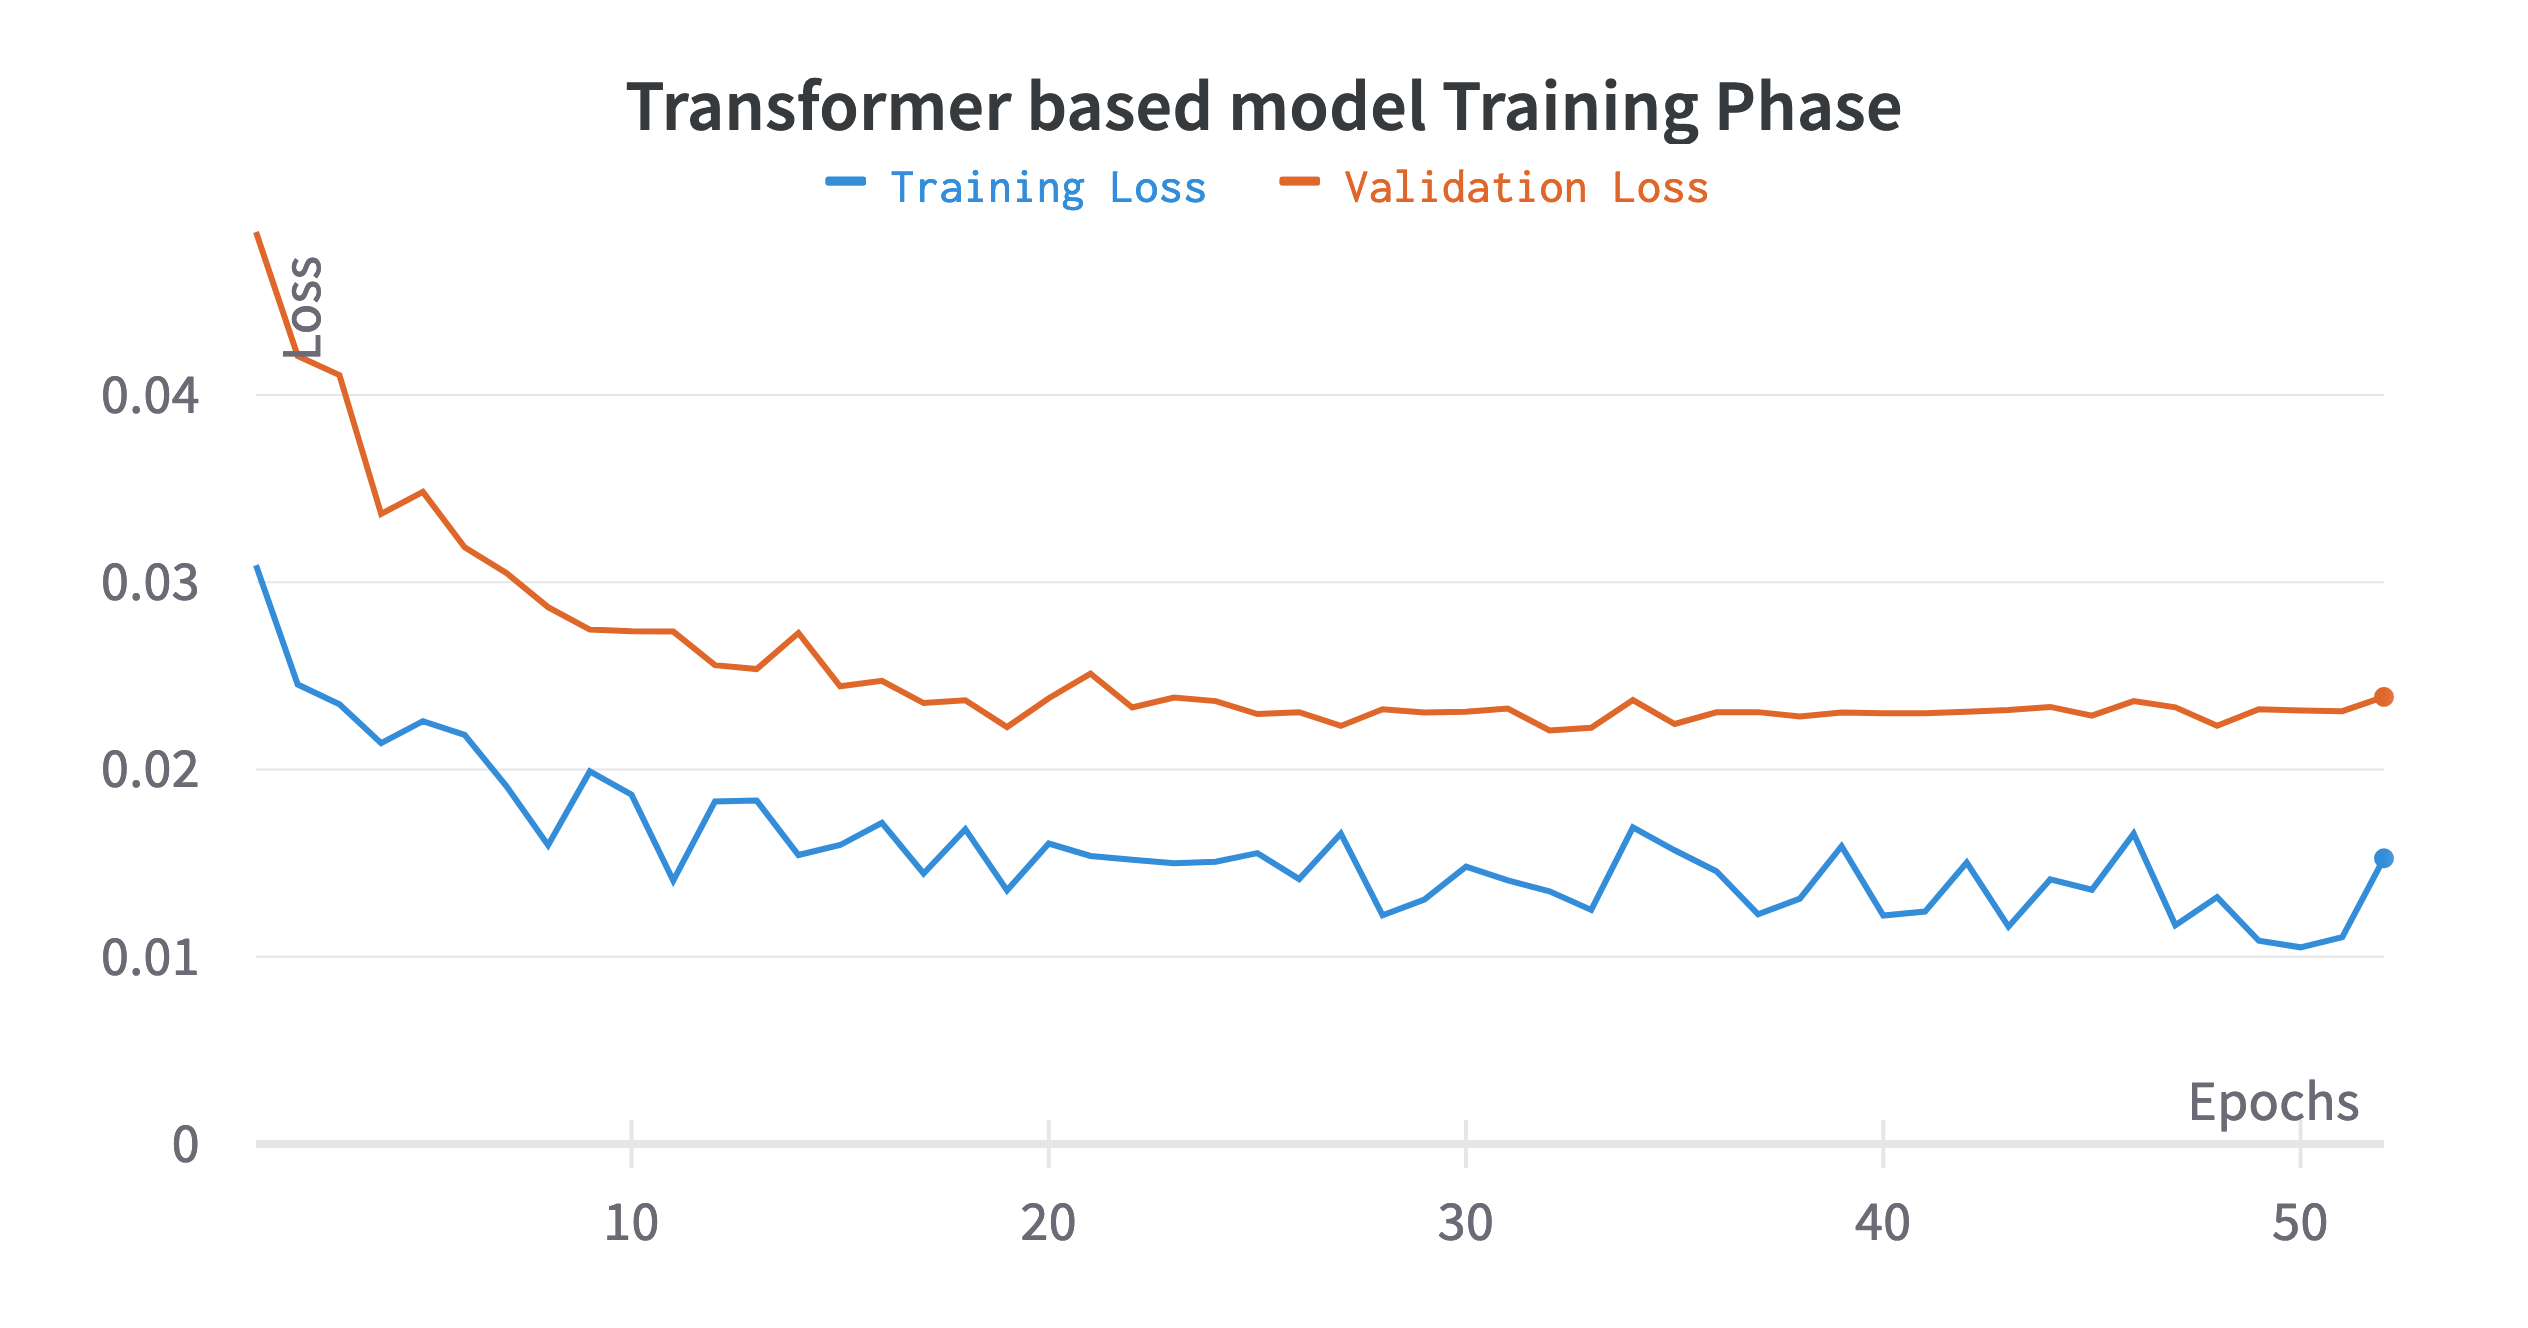
\includegraphics[width=.9\textwidth]{chapters/3_models/imgs/gab/gabtraining.png}
	\caption{The chart displays the loss progression during the training phase.The blue line represents the Training Loss, while the orange line represents the Validation Loss.}
	\label{fig:gabtrainchart}
\end{figure}

\begin{figure}[H]
	\centering
	\begin{subfigure}{0.43\textwidth}
		\centering
		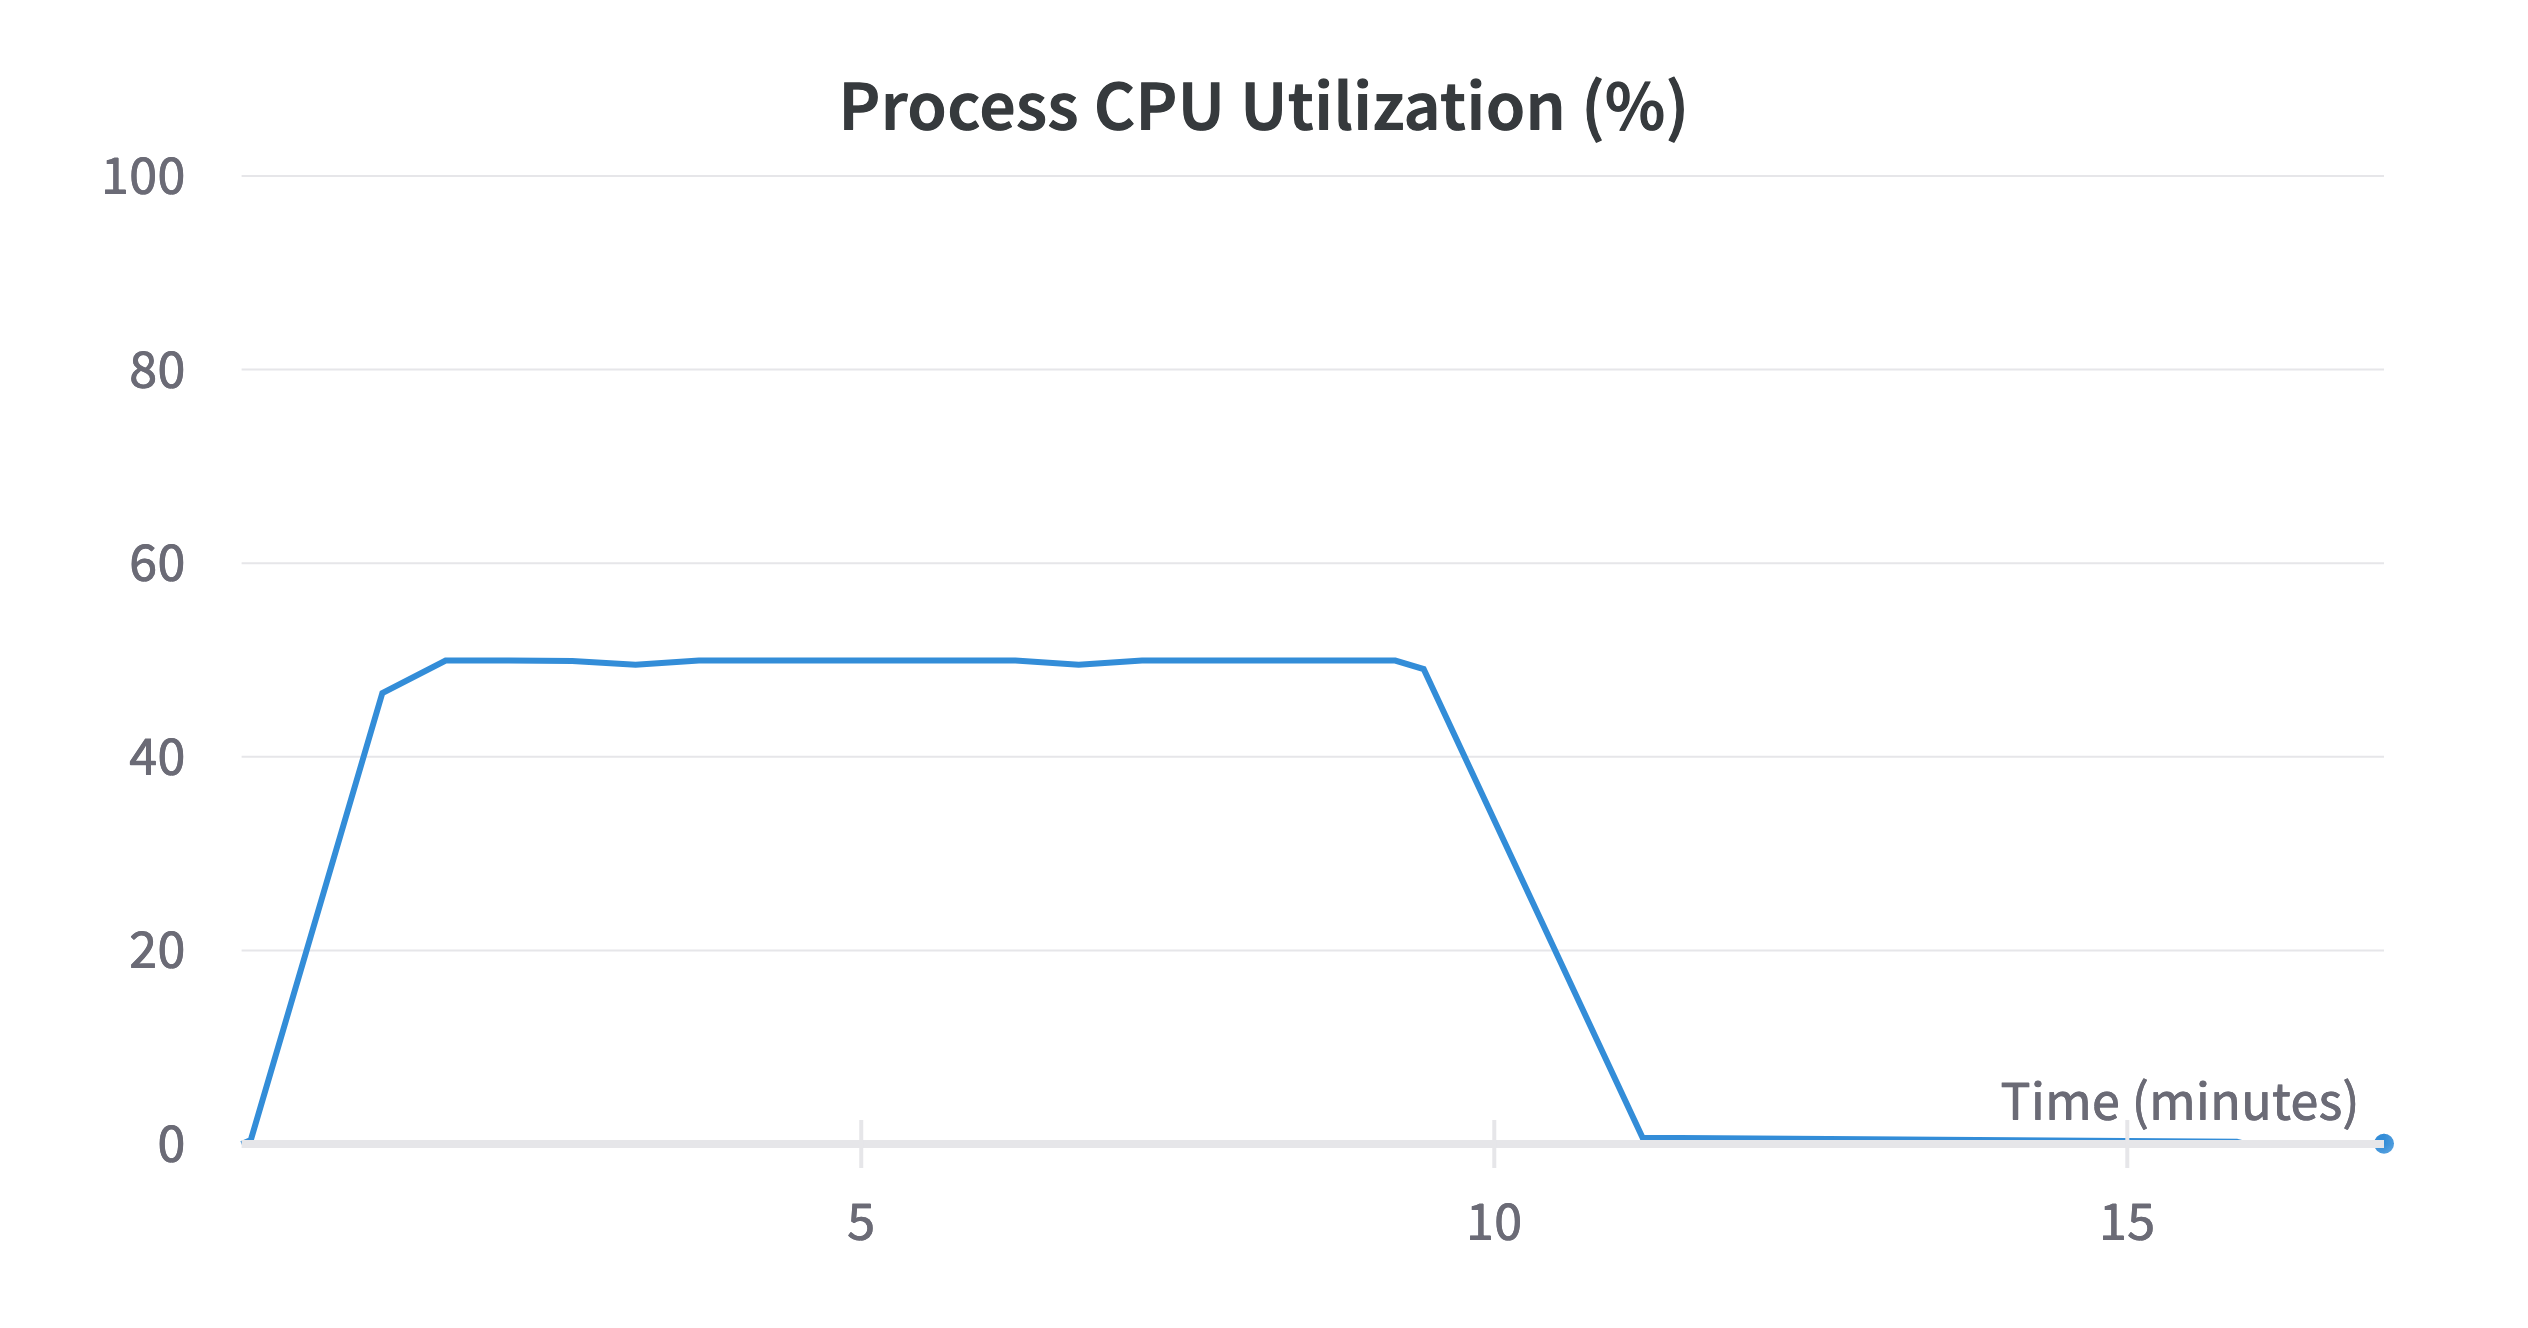
\includegraphics[width=\textwidth]{chapters/3_models/imgs/gab/train/gabrielcputilization.png}
	\end{subfigure}
	\begin{subfigure}{0.43\textwidth}
		\centering
		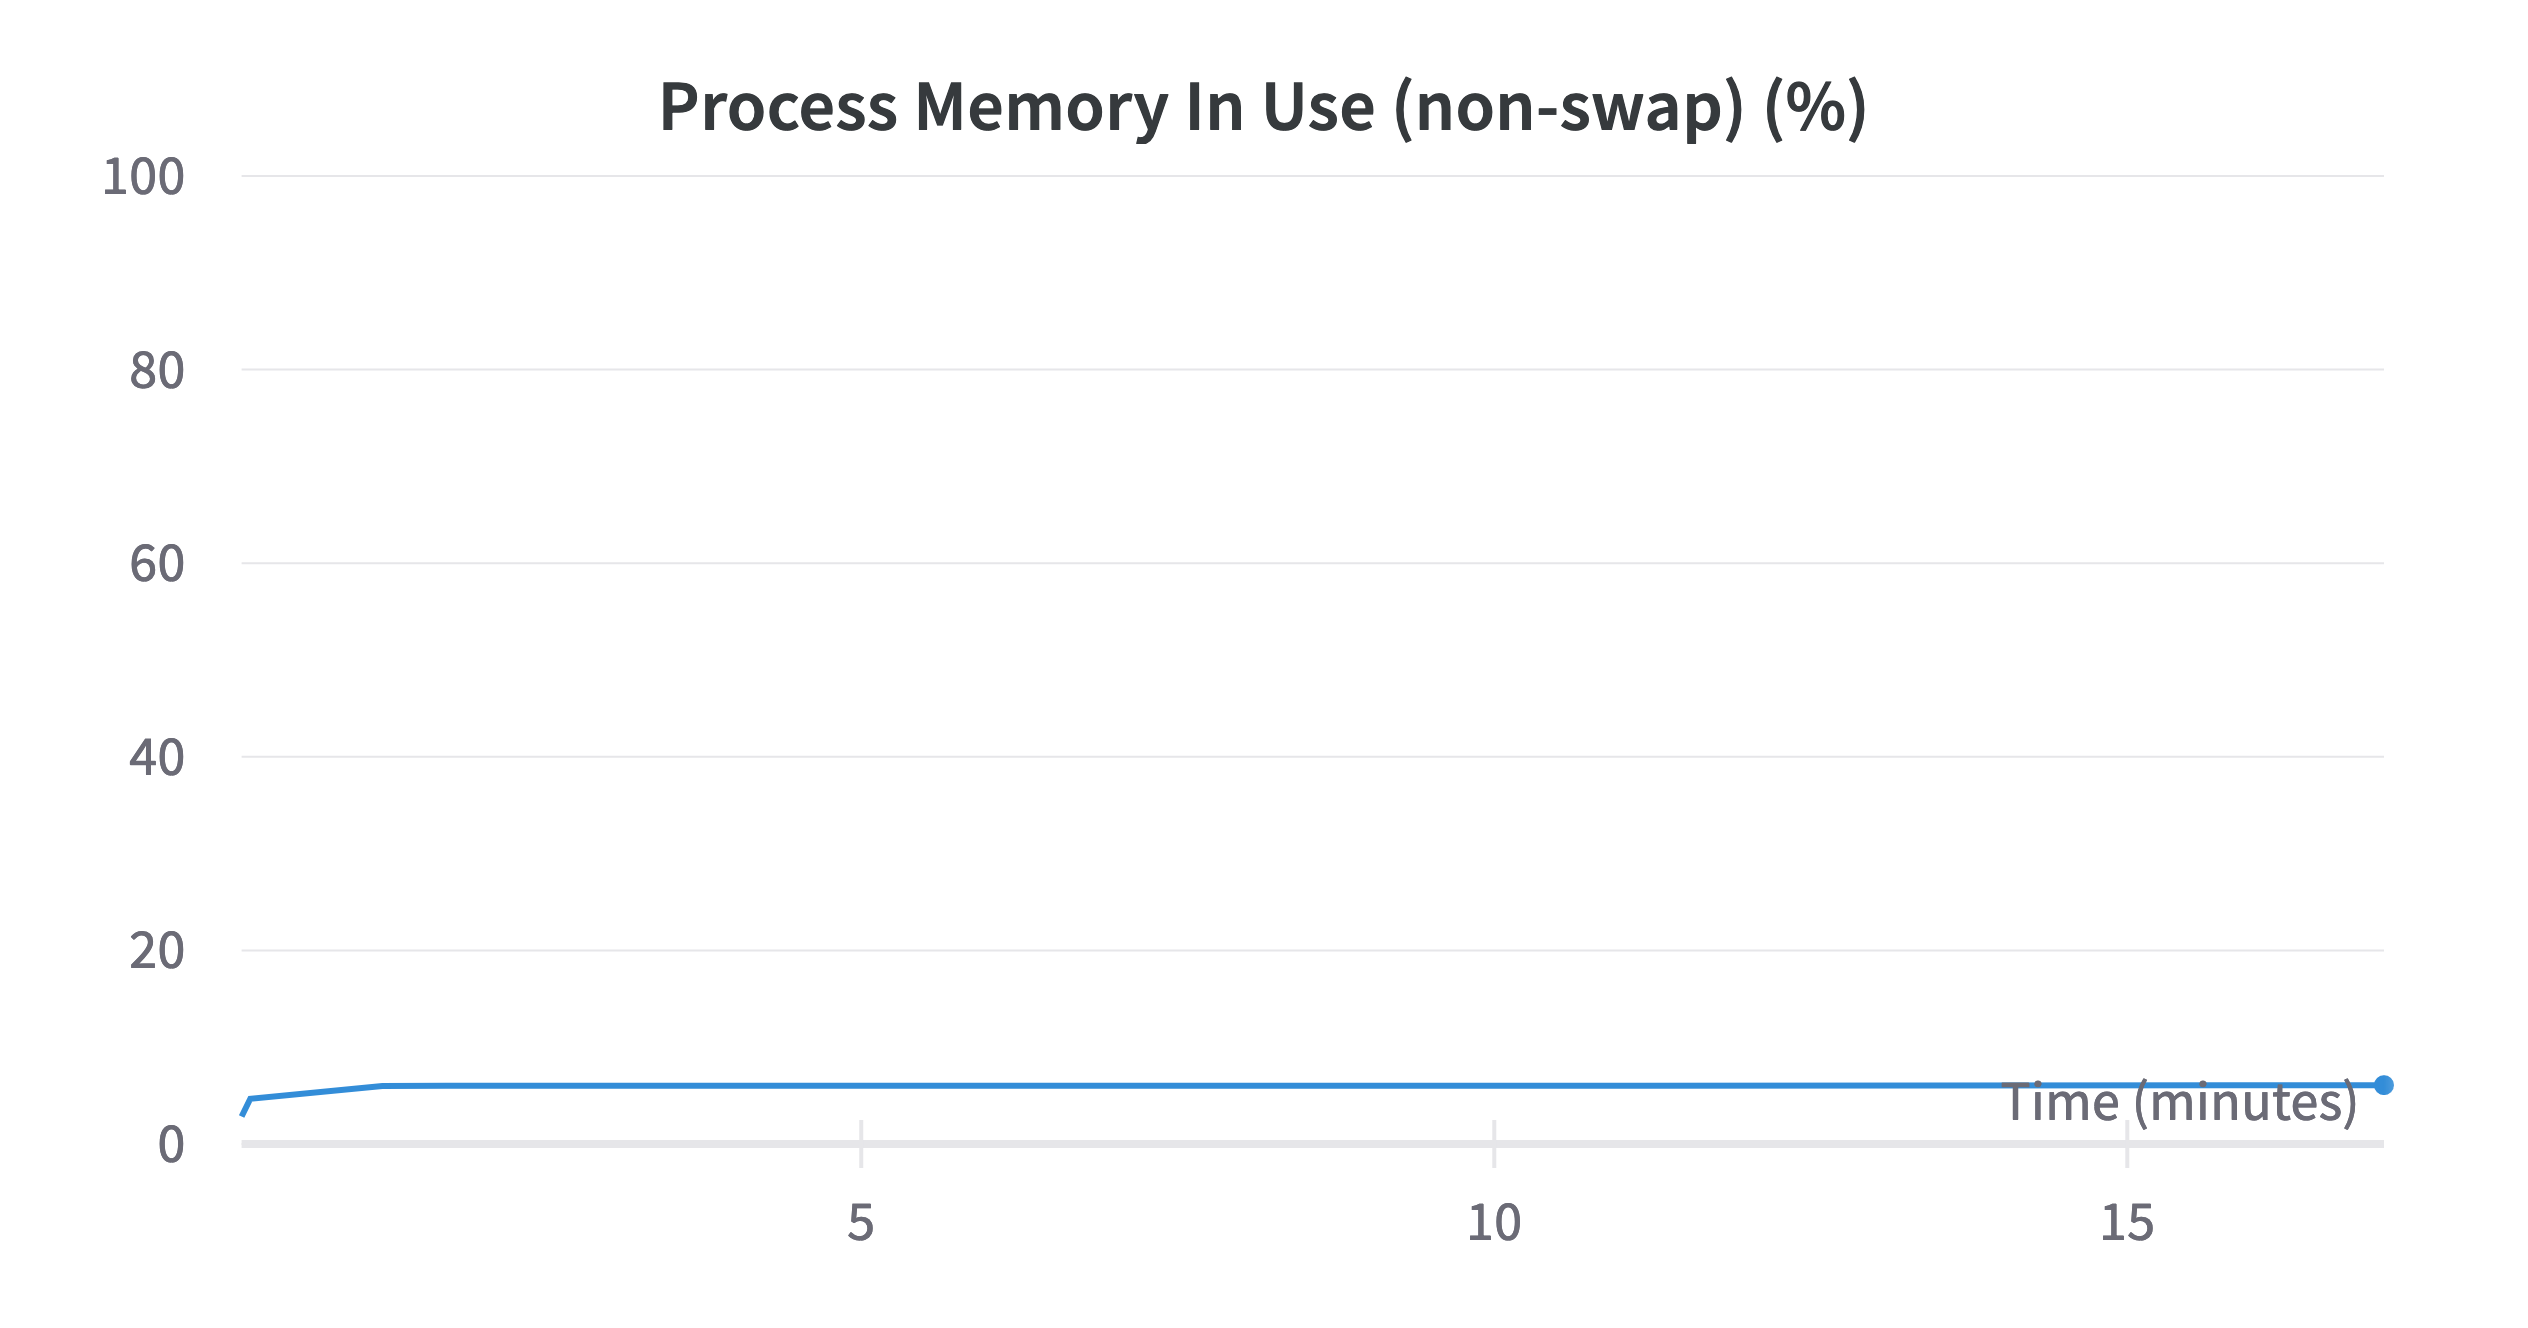
\includegraphics[width=\textwidth]{chapters/3_models/imgs/gab/train/gabrielprocessmemory.png}
	\end{subfigure}\\
	\begin{subfigure}{0.43\textwidth}
		\centering
		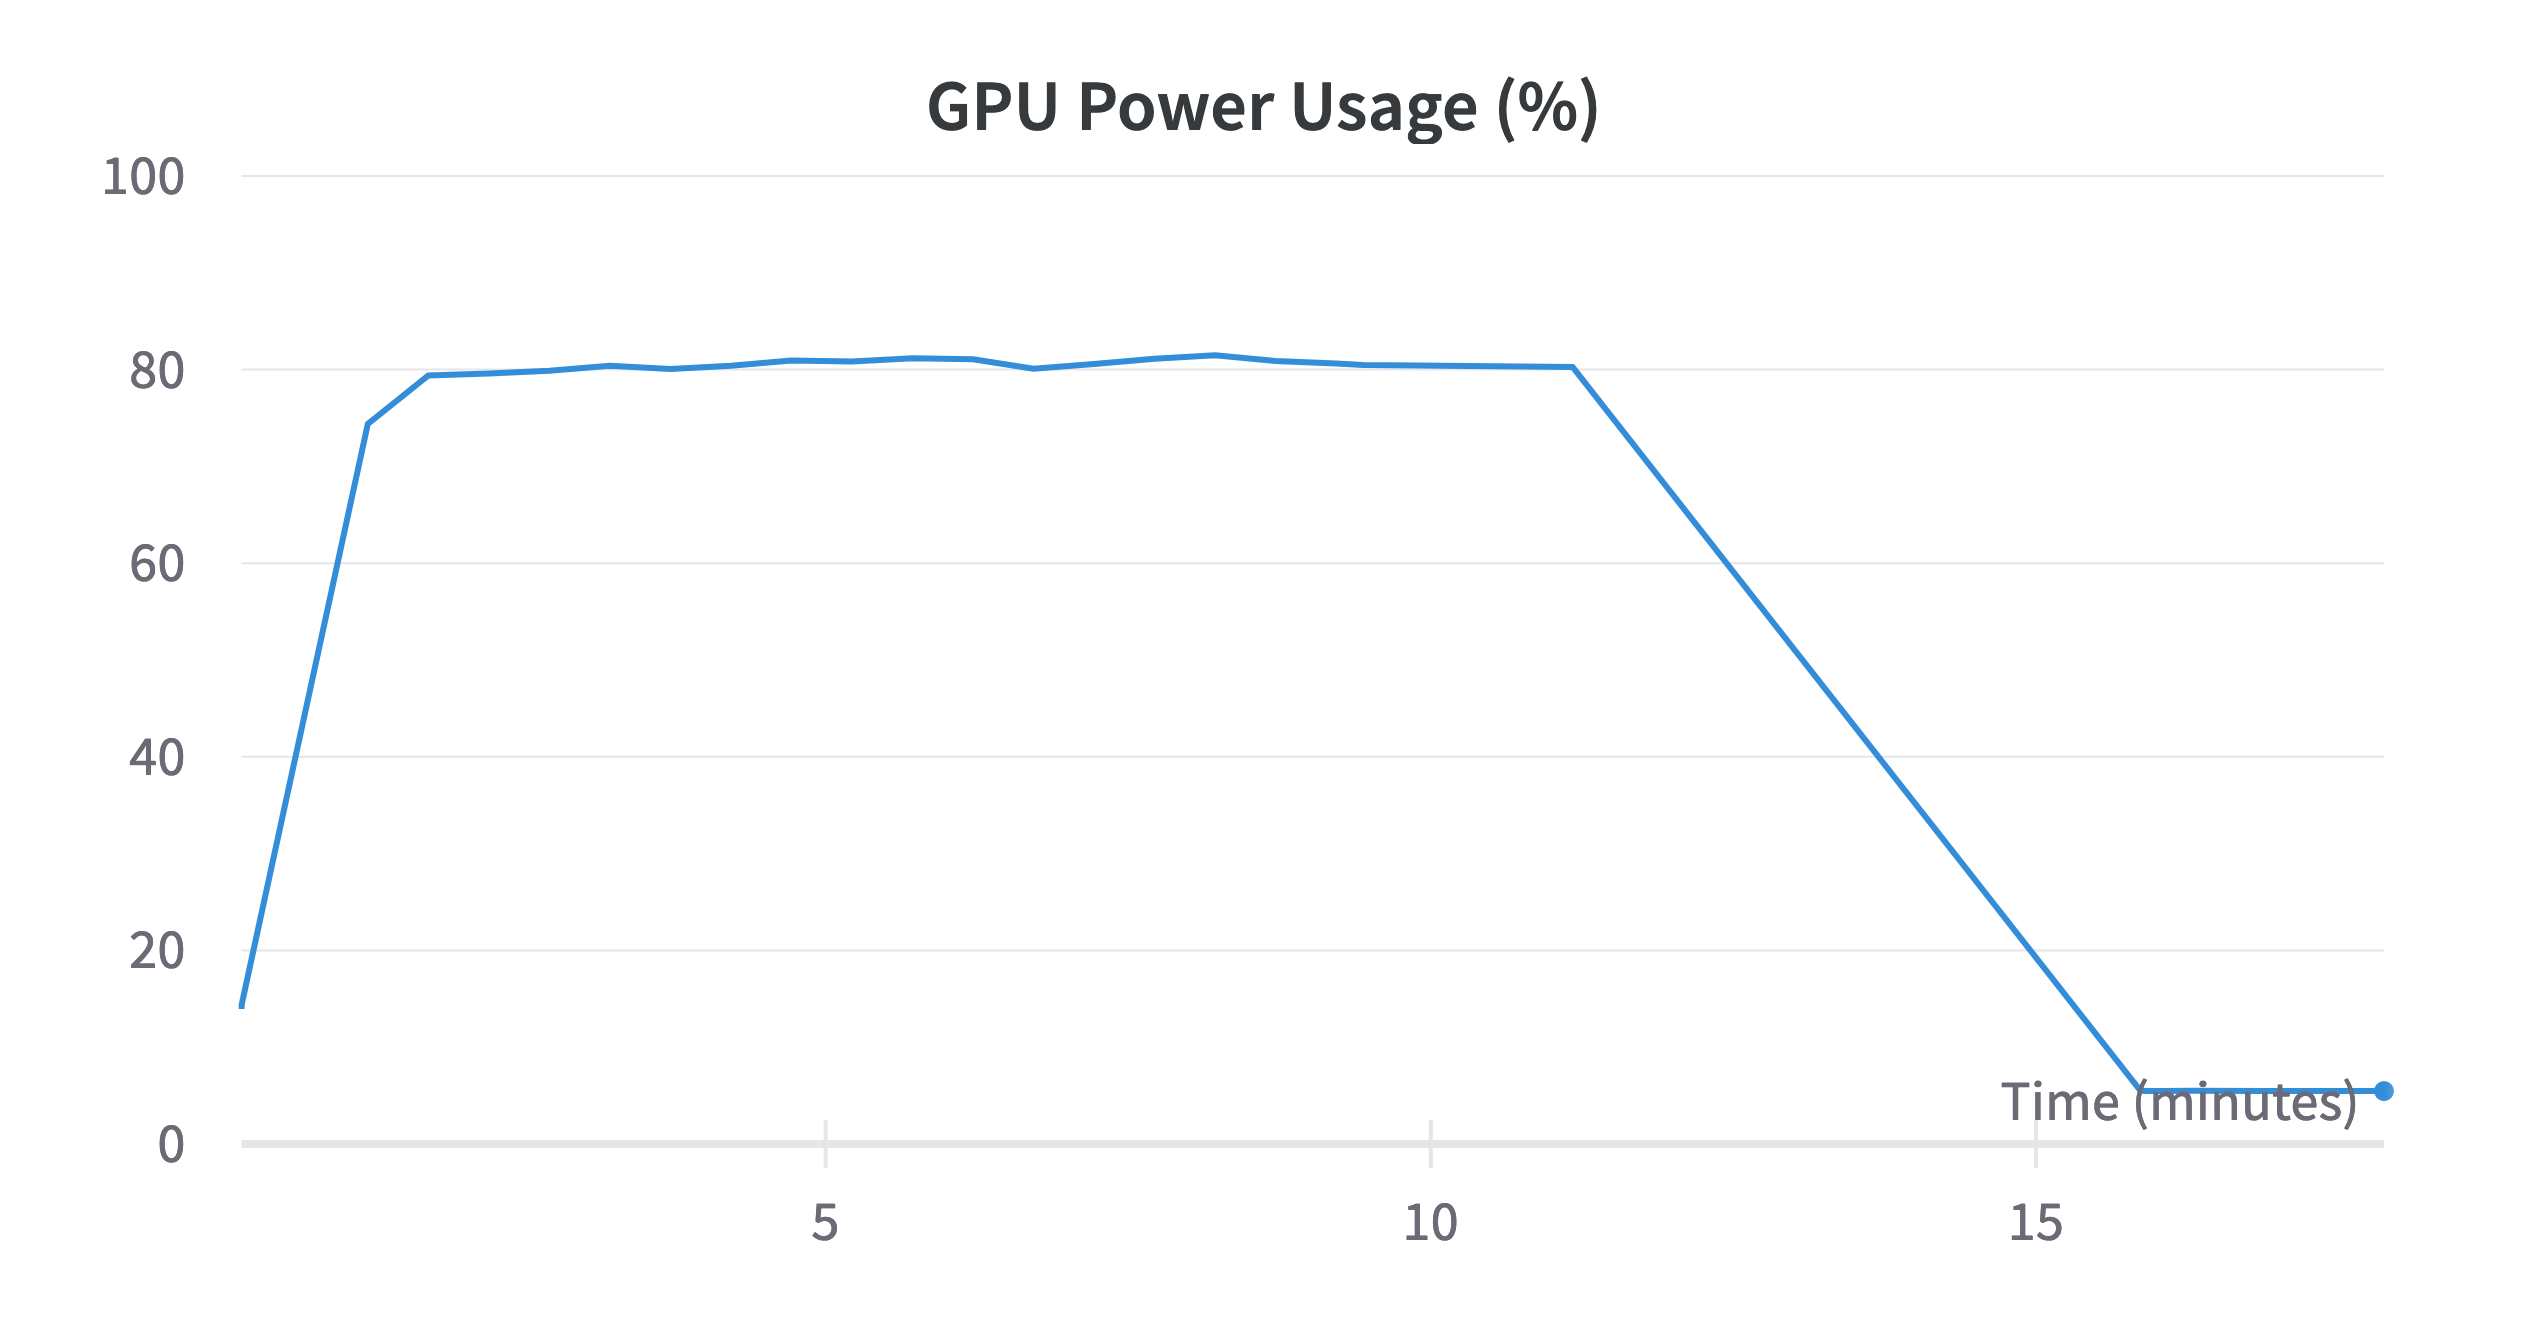
\includegraphics[width=\textwidth]{chapters/3_models/imgs/gab/train/gabrielgpupowerusageperc.png}
	\end{subfigure}
	\begin{subfigure}{0.43\textwidth}
		\centering
		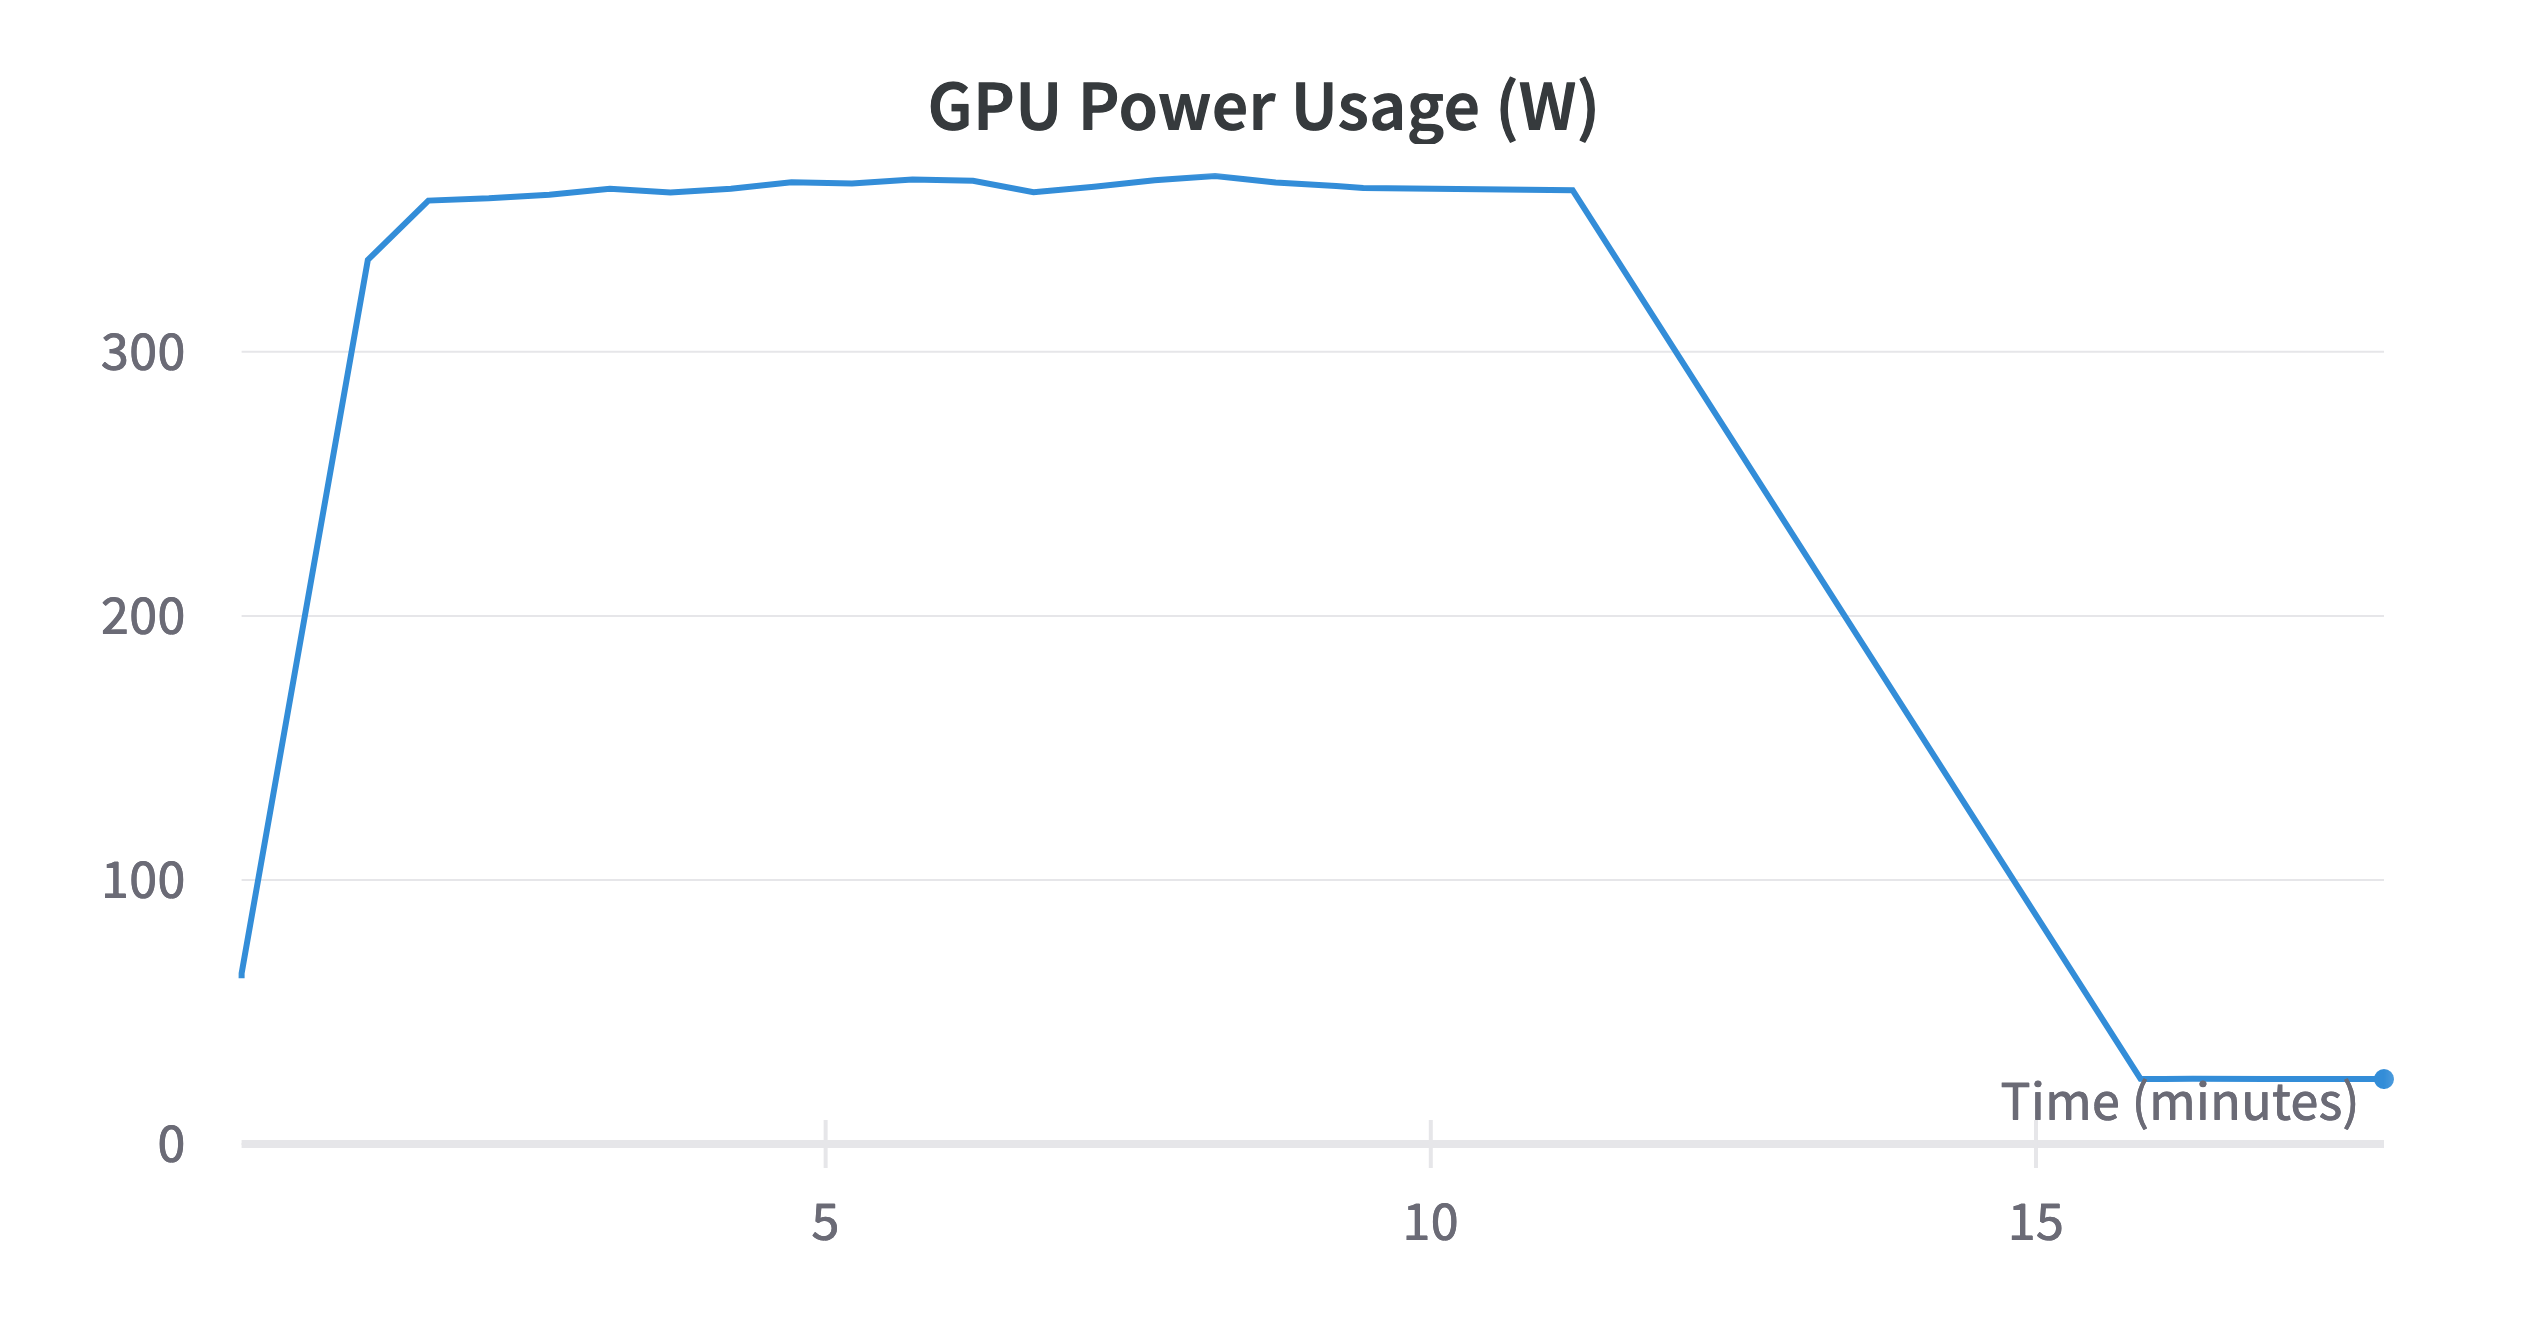
\includegraphics[width=\textwidth]{chapters/3_models/imgs/gab/train/gabrielgpupowerusagew.png}
	\end{subfigure}\\
	\begin{subfigure}{0.43\textwidth}
		\centering
		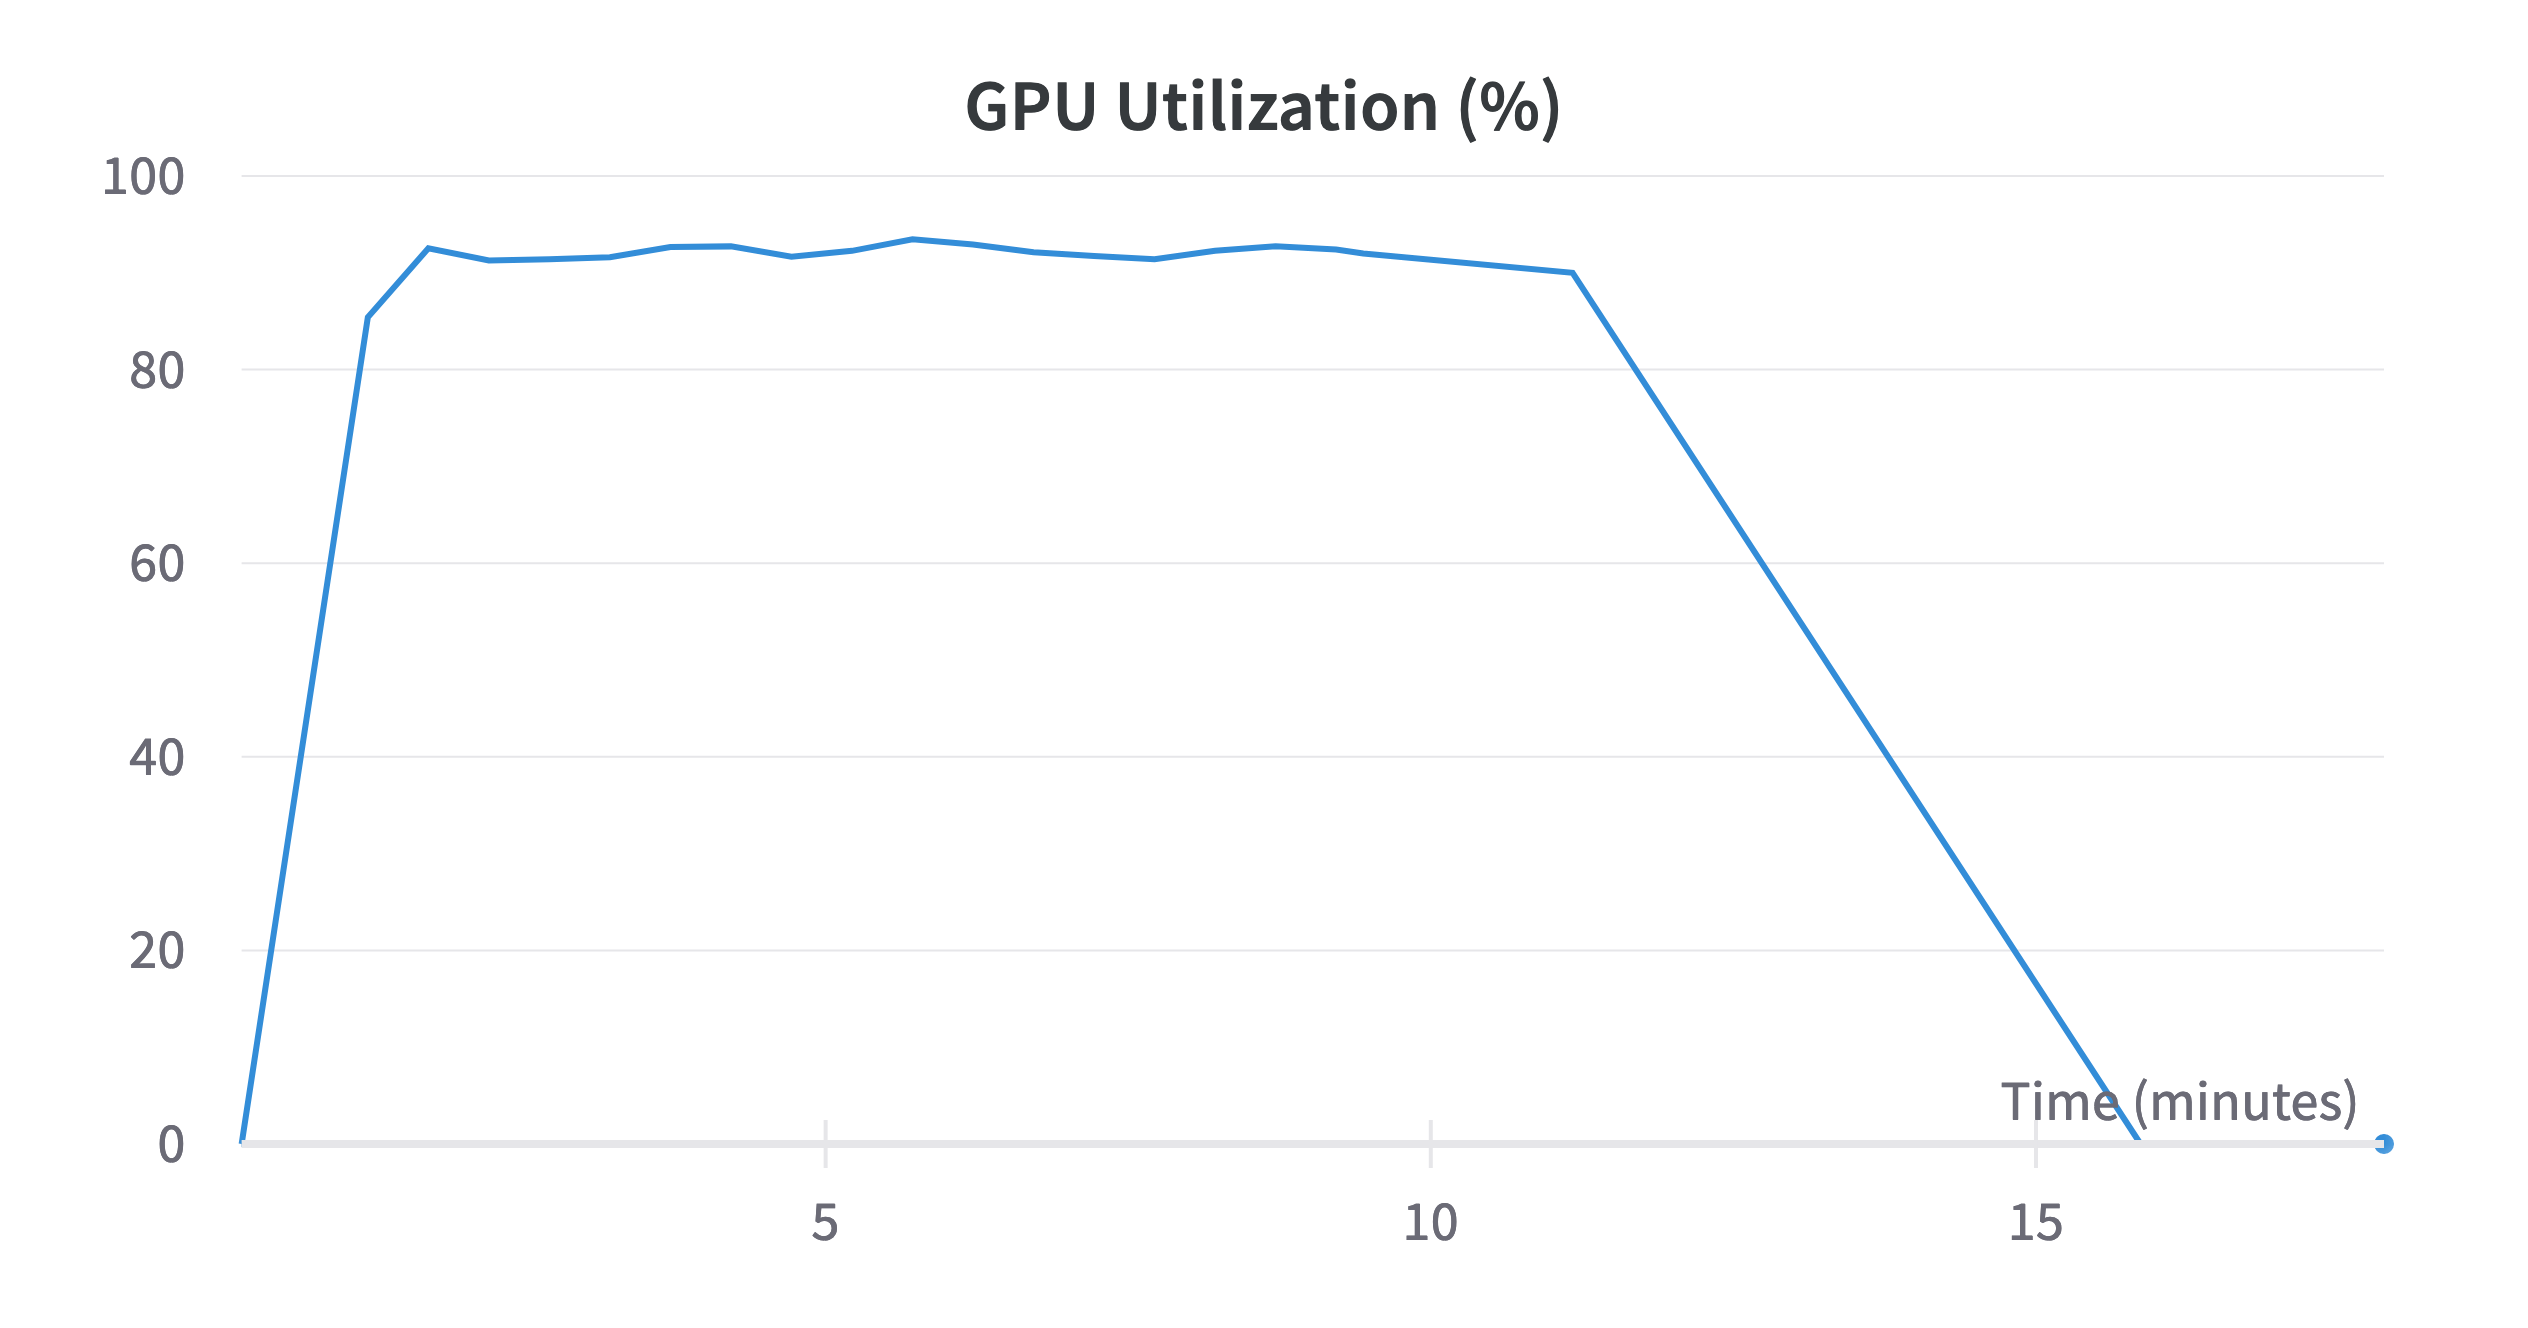
\includegraphics[width=\textwidth]{chapters/3_models/imgs/gab/train/gabrielgpuutilizationperc.png}
	\end{subfigure}
	\begin{subfigure}{0.43\textwidth}
		\centering
		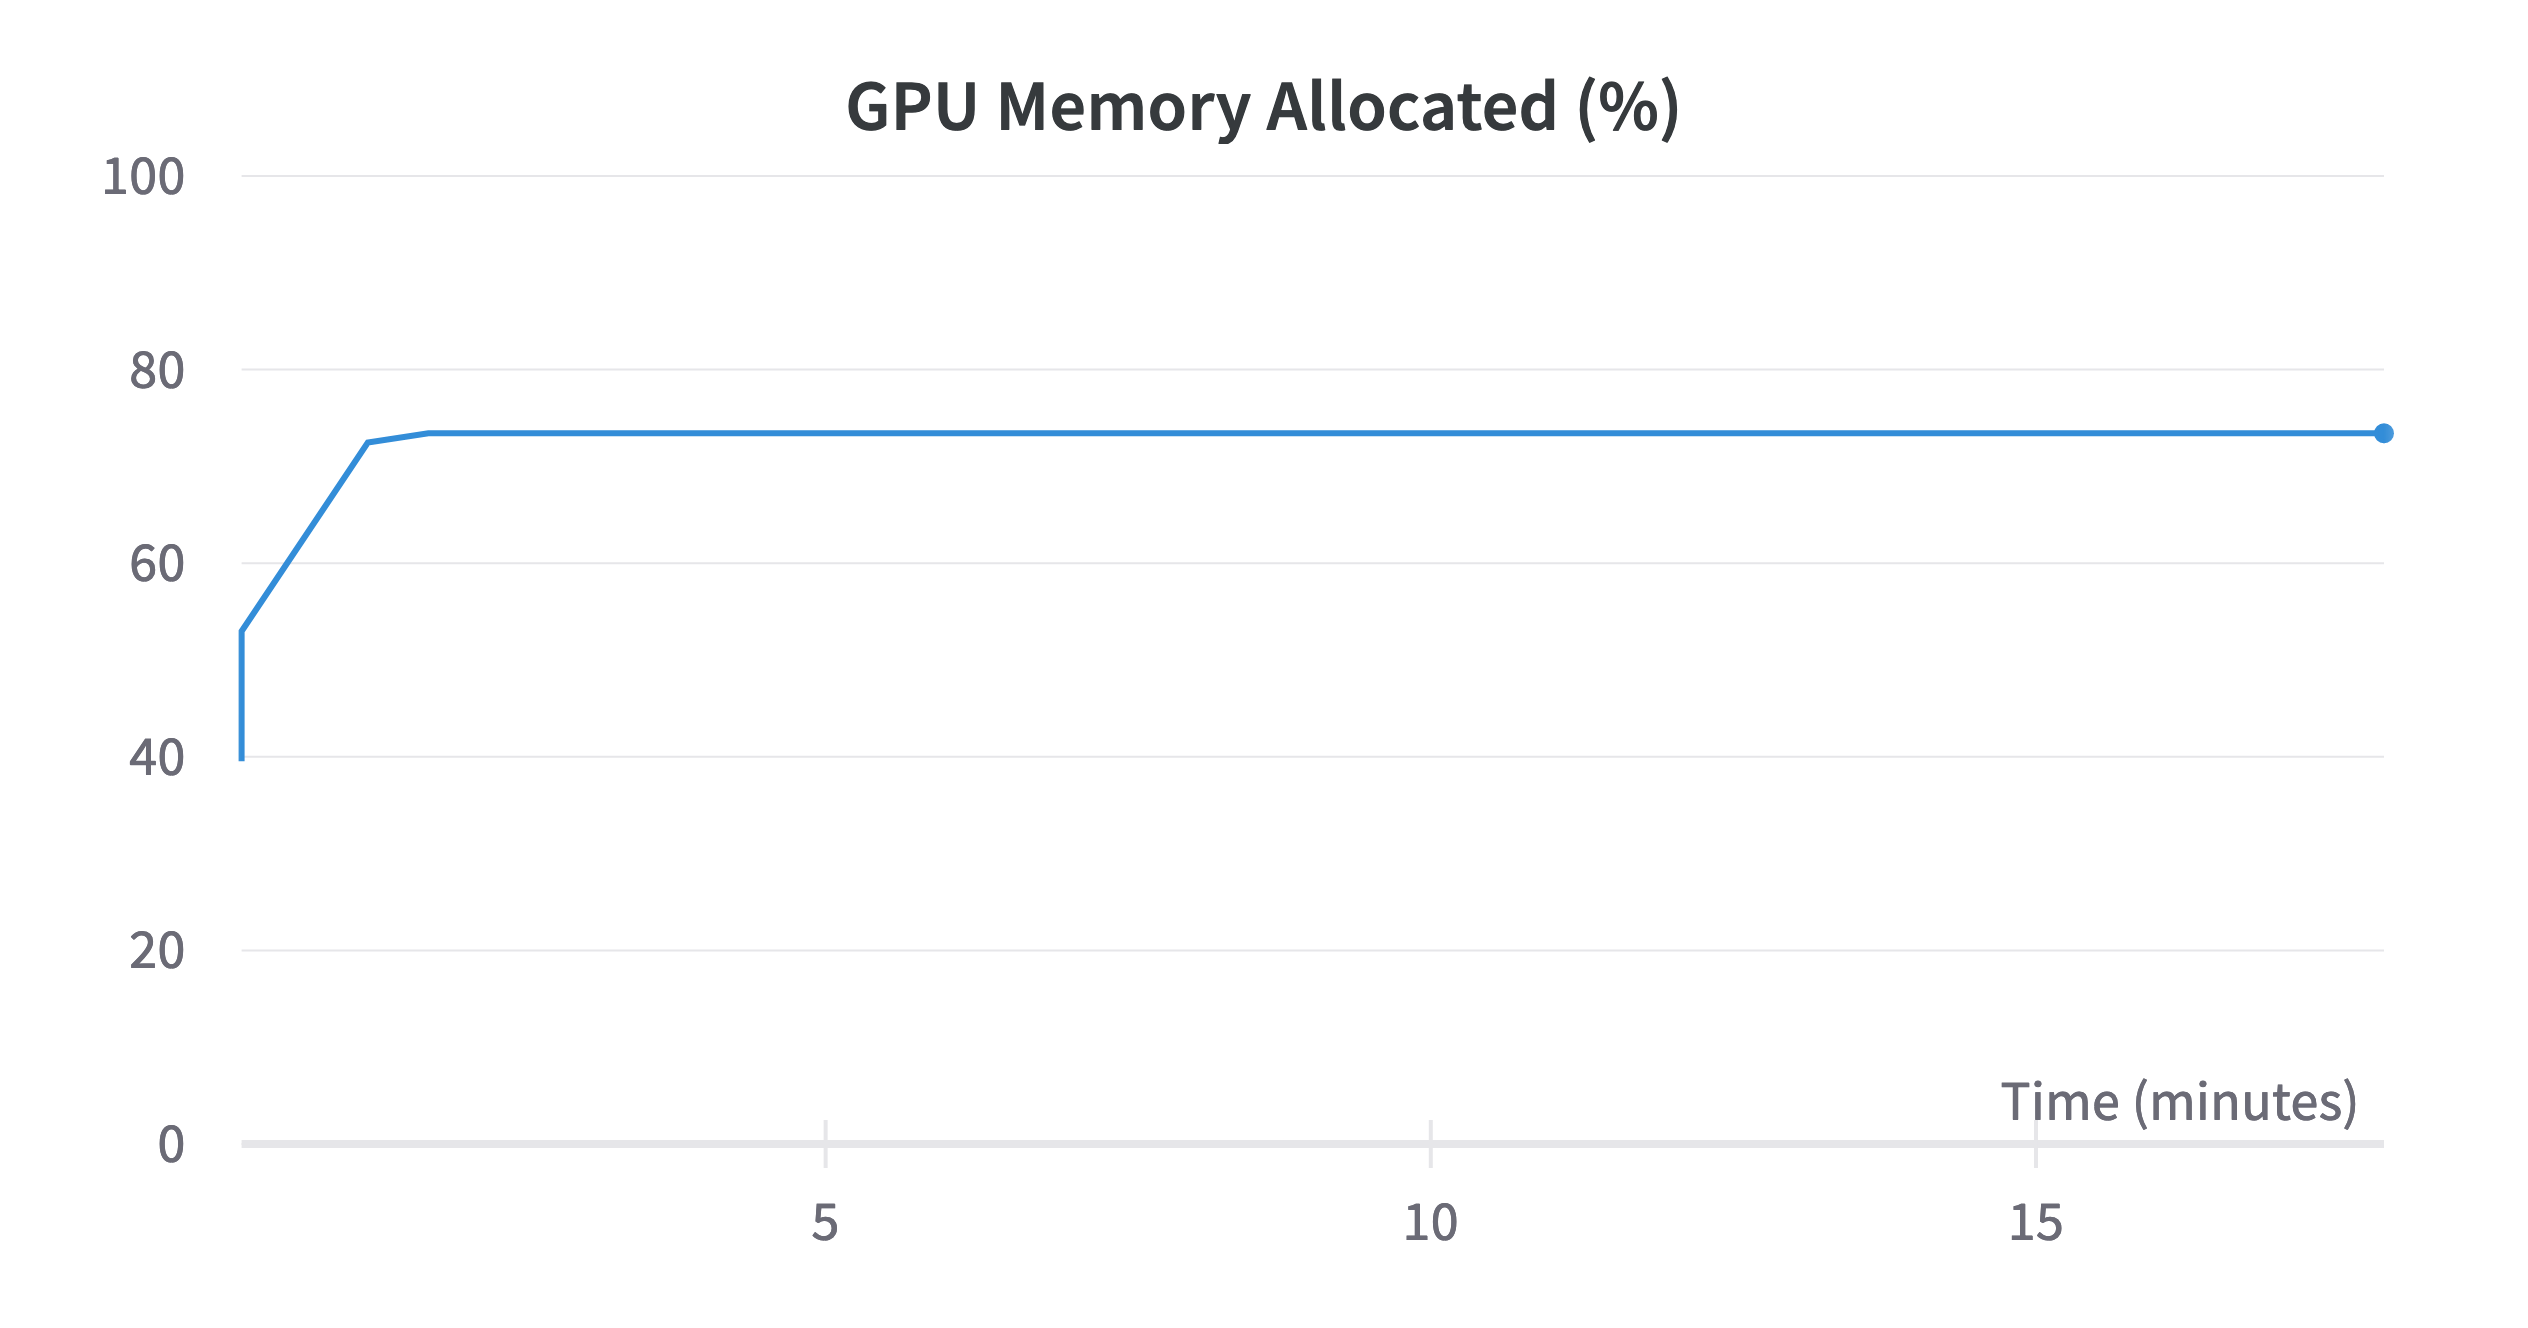
\includegraphics[width=\textwidth]{chapters/3_models/imgs/gab/train/gabrielgpumemalloc.png}
	\end{subfigure}\\
	\caption{System resources utilized during the Training phase.}
	\label{fig:gabsysusage}
\end{figure}


\begin{algorithm}[H]
	\caption{Transformer based model Training Algorithm}\label{alg:gabtraining}
	\begin{algorithmic}
		\Require train/validation datasets; Transformer based Neural Network Model

		\State Batch Size $\gets$ 8
		\State Learning Rate $\lambda \gets$ 0.00001
		\State Epochs $\gets$ 100
		\State Patience $\gets$ 20
		\State loss $\gets$ L1Loss()
		\State Optimizer $\gets$ AdamW Optimizer
		\State Scheduler $\gets$ CosineAnnealingScheduler
		\State Min Gap size $\gets$ 2 timestamps
		\State Max Gap size $\gets$ $\frac{\text{week length}}{3}$ timestamps
		\State
		\For{\textbf{each} epoch \textbf{in} epochs}
		\For{\textbf{each} (batch\_id, src\_data, tgt\_data, mask) \textbf{in} train.next\_batch()}

		\State train\_prediction $\gets$ model(src\_data) \Comment{Model inference}
		\State train\_prediction $\gets$ train\_prediction $\cdot$ mask
		\State train\_prediction $\gets \frac{\text{train\_prediction} \cdot \sum\text{train\_prediction}}{\sum tgt\_data}$ \Comment{Area normalization}
		\State train\_loss $\gets$ loss(train\_prediction[mask = 1], tgt\_data[mask = 1])
		\State Optimizer step
		\State Back Propagation
		\EndFor
		\State Scheduler step
		\State stop computing gradient
		\For{\textbf{each} (batch\_id, vs, vt, vm) \textbf{in} validation.next\_batch()}
		\State val\_prediction $\gets$ model(vs) \Comment{Model inference}
		\State val\_prediction $\gets$ val\_prediction $\cdot$ vm
		\State val\_prediction $\gets \frac{\text{val\_prediction} \cdot \sum\text{val\_prediction}}{\sum vt}$ \Comment{Area normalization}
		\State val\_loss $\gets$ loss(val\_prediction[vm = 1], vt[vm = 1])
		\EndFor

		\State check for Early Stopping
		\State check for Save Best Result
		\State start computing gradient
		\EndFor
	\end{algorithmic}
\end{algorithm}
\newpage
From the graph shown in Figure~\ref{fig:gabtrainchart}, we can observe that the training and validation loss curves, after an initial descent, remain relatively constant, and most importantly, they do not seem to diverge from each other. This indicates that the training phase has concluded successfully, with the validation loss value being lower by 0.01 compared to the RNN-based model.

From the graphs in Figure~\ref{fig:gabsysusage}, which show the machine's usage during the training phase, and from Table~\ref{tab:gabspecs}, it can be inferred that the model utilizes almost all of the available hardware resources, suggesting that it is computationally intensive and might be challenging to train on less powerful machines. However, it's essential to note that the inference time is extremely fast, not exceeding one second, and the model file size is very compact, with a dimension of approximately 2 MB.
